%%%%%%%%%%%%%%%%%%%%%%%%%%%%%%%%%%%%%%%%%%%%%%%%%%%%%%%%%%%%%%%%%%%%%%%%%%%%%%%
%%                                                                           %%
%%   Dr Varun Ojha                                                           %%
%%   Lecturer, Department of Computer Science                                %%
%%   University of Reading, UK                                               %%
%%                                                                           %%
%%%%%%%%%%%%%%%%%%%%%%%%%%%%%%%%%%%%%%%%%%%%%%%%%%%%%%%%%%%%%%%%%%%%%%%%%%%%%%%
%%%%     SETTING STARTS - DO NOT CHANGE Unless your TeX setting require so   %%
%%%%%%%%%%%%%%%%%%%%%%%%%%%%%%%%%%%%%%%%%%%%%%%%%%%%%%%%%%%%%%%%%%%%%%%%%%%%%%%
%%----------------------------------------------------------------------------------
% DO NOT Change this. It is the required setting A4 page, 11pt, onside print,
% book style
%%----------------------------------------------------------------------------------
\documentclass[a4paper,11pt,twoside]{book}
\renewcommand{\baselinestretch}{1.0}


%%-------------------------------------
%% Page margin settings - % half inch margin all sides (recommended)
%%-------------------------------------
\usepackage[inner=4cm,outer=3cm]{geometry} 

%%-------------------------------------
%% Font settings - % CM San or Ariel (recommended)
%%-------------------------------------
% Switch the following two line off: to revert back to default LaTex font (NOT
% recommended)
\usepackage{amsfonts}
\renewcommand*\familydefault{\sfdefault}

%%-------------------------------------
%% Math/Definition/Theorem/Algorithm packages settings 
%%-------------------------------------
\usepackage[cmex10]{amsmath}
\usepackage{amssymb}
\usepackage{amsthm}
\newtheorem{mydef}{Definición}
\newtheorem{mytherm}{Theorem}
\newtheorem{theorem}{Theorem}[section]
\newtheorem{corollary}{Corollary}[theorem]
\newtheorem{lemma}[theorem]{Lemma}
\newenvironment{conditions}
  {\par\vspace{\abovedisplayskip}\noindent\begin{tabular}{>{$}l<{$} @{${}={}$} l}}
  {\end{tabular}\par\vspace{\belowdisplayskip}}

\usepackage{multicol}

%%-------------------------------------
%% Algorithms/Code Listing environment settings  - % Please do not change these
%settings
%%-------------------------------------
\usepackage{algorithm}
\usepackage{algpseudocode}
\renewcommand{\algorithmicrequire}{\textbf{Input:}}
\renewcommand{\algorithmicensure}{\textbf{Output:}}
\newcommand{\vect}[1]{\boldsymbol{#1}}
\usepackage[utf8]{inputenc}
\usepackage{listings}
\usepackage{xcolor}
\usepackage[spanish]{babel}
\definecolor{codegreen}{rgb}{0,0.6,0.1}
\definecolor{codegray}{rgb}{0.5,0.5,0.5}
\definecolor{codeblue}{rgb}{0.10,0.00,1.00}
\definecolor{codepurple}{rgb}{0.58,0,0.82}
\definecolor{backcolour}{rgb}{1.0,1.0,1.0}

\lstdefinestyle{mystyle}{backgroundcolor=\color{backcolour},   
    commentstyle=\color{codegreen}, keywordstyle=\color{codeblue},
    numberstyle=\tiny\color{codegray}, stringstyle=\color{codepurple},
    basicstyle=\ttfamily\footnotesize, breakatwhitespace=false,         
    breaklines=true,                 
    captionpos=b,                        
    keepspaces=true,                 
    numbers=left,                    
    numbersep=5pt,                  
    showspaces=false,                
    showstringspaces=false, showtabs=false,                  
    tabsize=2, frame=none}
\lstset{style=mystyle}

\lstdefinelanguage{PDDL}
{
  sensitive=false,    % not case-sensitive
  morecomment=[l]{;}, % line comment
  alsoletter={:,-},   % consider extra characters
  morekeywords={
    define,domain,problem,not,and,or,when,forall,exists,either,
    :domain,:requirements,:types,:objects,:constants,
    :predicates,:action,:parameters,:precondition,:effect,
    :fluents,:primary-effect,:side-effect,:init,:goal,
    :strips,:adl,:equality,:typing,:conditional-effects,
    :negative-preconditions,:disjunctive-preconditions,
    :existential-preconditions,:universal-preconditions,:quantified-preconditions,
    :functions,assign,increase,decrease,scale-up,scale-down,
    :metric,minimize,maximize,
    :durative-actions,:duration-inequalities,:continuous-effects,
    :durative-action,:duration,:condition
  }
}

%%-------------------------------------
%% Graphics/Figures environment settings
%%-------------------------------------
\usepackage{graphicx}
%\usepackage{subfigure}
\usepackage{caption}
\usepackage{lipsum}
\usepackage{subcaption}
%%-------------------------------------
%% Table environment settings
%%-------------------------------------
\usepackage{multirow}
\usepackage{rotating}
\usepackage{makecell}
\usepackage{booktabs}
%\usepackage{longtable,booktabs}

%%-------------------------------------
%% List of Abbreviations settings
%%-------------------------------------
\usepackage{enumitem}
\newlist{abbrv}{itemize}{1}
\setlist[abbrv,1]{label=,labelwidth=1in,align=parleft,itemsep=0.1\baselineskip,leftmargin=!}

\newcommand{\frontpagetoday}{\ifcase \month \or Enero\or Febrero\or Marzo\or %
Abril\or Mayo \or Junio\or Julio\or Agosto\or Septiembre\or Octubre\or Noviembre\or %
Diciembre\fi, \number \year} 

\usepackage[
    type={CC},
    modifier={by-sa},
    version={4.0},
    imagewidth={5cm}
]{doclicense}
%%-------------------------------------
%% Bibliography/References settings   - Harvard Style was used in this report
%%-------------------------------------
\usepackage[hidelinks]{hyperref}
\usepackage[comma,authoryear]{natbib}
\renewcommand{\bibname}{References} % DO NOT remove or switch of 

%%-------------------------------------
%% Appendix settings     
%%-------------------------------------
\usepackage[toc]{appendix}
%%%%%%%%%%%%%%%%%%%%%%%%%%%%%%%%%%%%%%%%%%%%%%%%%%%%%%%%%%%%%%%%%%%%%%%%%%%%%%%%%%%%%%%
%%%%                     SETTING ENDS
%%%%%%%
%%%%%%%%%%%%%%%%%%%%%%%%%%%%%%%%%%%%%%%%%%%%%%%%%%%%%%%%%%%%%%%%%%%%%%%%%%%%%%%%%%%%%%%
\begin{document}

    \SetLipsumDefault{1}
    
\frontmatter

\begin{titlepage}      
    \begin{center}
        % University
        {\huge
            Universidad Nacional de Córdoba
            
            \vspace{0.8cm}
            
            Facultad de Matemática, Astronomía, Física, y Computación
        }\\[1cm]
        % Logo
        
\includegraphics[width=0.4\textwidth]{./figures/logo_unc.png}
        
        \vspace*{1cm}
        
        % Title
        \begin{tabular}{@{}p{\textwidth}@{}}
        \toprule[2pt]
        \midrule
        \vspace{0.2cm}
        \begin{center}
        \Huge{\textbf{Uso de Planes Relajados en Grounding Heurístico}}
        \end{center}
        \vspace{0.2cm}\\
        \midrule
        \toprule[2pt]
        \end{tabular}

        \linespread{1}~\\[1cm]

        % Author and supervisors
        {\Large
            \emph{Autor:} Nicolás Benjamín Ocampo
        }\\[1cm]
        {\Large
            \emph{Directores:} Dr. Carlos Areces y Dr. Martín Dominguez
        }\\[1cm]
        
        % Degree of the defence
        \vfill
        \Large \emph{Trabajo de tesis presentado para obtener el título de
        Licenciado en Ciencias de la Computación}\\[0.3cm] 
        
        \vspace{0.8cm}
        \vspace{0.8cm}
        
        \today
    \end{center}
\end{titlepage}
    
    \newpage
    
    
    % To my family

    %\begin{center}
    %   \hspace{0pt}
    %   \vfill
    %   \emph{Dedicado a mi familia, \\
    %    por siempre estar conmigo durante esta hermosa etapa de mi vida \\
    %    ...Mil gracias por todo...}
    %   \vfill
    %   \hspace{0pt}
    %\end{center}
     
    % -------------------------------------------------------------------
    % Abstract and Acknowledgement
    % -------------------------------------------------------------------
    
    %Two resources useful for abstract writing.
% Guidance of how to write an abstract/summary provided by Nature: https://cbs.umn.edu/sites/cbs.umn.edu/files/public/downloads/Annotated_Nature_abstract.pdf %https://writingcenter.gmu.edu/guides/writing-an-abstract
\chapter*{\center \Large  Abstract}
%%%%%%%%%%%%%%%%%%%%%%%%%%%%%%%%%%%%%%
% Replace all text with your text
%%%%%%%%%%%%%%%%%%%%%%%%%%%%%%%%%%%

This is an undergraduate project report template and instruction on how to write a report. It also has some useful examples to use \LaTeX. Do read this template carefully. The number of chapters and their titles may vary depending on the type of project and personal preference. Section titles in this template are illustrative should be updated accordingly. For example, sections named ``A section...'' and ``Example of ...'' should be updated. The number of sections in each chapter may also vary. This template may or may not suit your project. Discuss the structure of your report with your supervisor.

%%%
~\\[1cm]%REMOVE THIS
\noindent\textbf{Guidance on abstract writing:} An abstract is a summary of a report in a single paragraph up to a maximum of 250 words. An abstract should be self-contained, and it should not refer to sections, figures, tables, equations, or references. An abstract typically consists of sentences describing the following four parts: (1) introduction (background and purpose of the project), (2) methods, (3) results and analysis, and (4) conclusions. The distribution of these four parts of the abstract should reflect the relative proportion of these parts in the report itself. An abstract starts with a few sentences describing the project's general field, comprehensive background and context, the main purpose of the project; and the problem statement. A few sentences describe the methods, experiments, and implementation of the project. A few sentences describe the main results achieved and their significance. The final part of the abstract describes the conclusions and the implications of the results to the relevant field.


%%%%%%%%%%%%%%%%%%%%%%%%%%%%%%%%%%%%%%%%%%%%%%%%%%%%%%%%%%%%%%%%%%%%%%%%%s
~\\[1cm]
\noindent % Provide your key words
\textbf{Keywords:} a maximum of five keywords/keyphrase separated by commas

\vfill
\noindent
\textbf{Report's total word count:} we expect a maximum of 20,000 words (excluding reference and appendices) and about 50 - 60 pages. [A good project report can also be written in approximately 10,000 words.]


    % -------------------------------------------------------------------
	% Acknowledgement
	% -------------------------------------------------------------------
   
    \chapter*{\center \Large  Agradecimientos}
Esta tesis es fruto del trabajo y colaboración de un montón de personas que
compartieron conmigo su grano de arena durante mi formación.

Empezando por mi familia que me acompañó en mi decisión de mudarme a la ciudad
de Córdoba y seguir esta carrera que me ha enseñado tanto. A todos mis hermanos
que a pesar de verlos una vez al año por tan solo algunas semanas, logran
compartir sus cariño que se queda conmigo durante el resto de la temporada.

A mis directores, Carlos y Martín que me brindaron su paciencia, tiempo, y
conocimiento haciéndome sentir realmente cómodo y seguro durante el desarrollo
de esta tesis. 

A mis amigos que fueron mi cable a tierra en numerosas ocasiones. Juntarse con
ellos, para compartir risas, experiencias, o simplemente matar el rato, es algo
que no tiene precio.

TODO: Continuar.   
    
    % -------------------------------------------------------------------
    % Contents, list of figures, list of tables
    % -------------------------------------------------------------------
    
    \tableofcontents
    
    \mainmatter
    
    \chapter{Introducción}
\label{ch:into}

La planificación automática, o simplemente \emph{Planning}, es una de las áreas
centrales de la inteligencia artificial debido a su extenso uso en dominios,
tales como, control de misiones espaciales \citep{RabideauG-et-al-2001}, manejo
de crisis \citep{Bienkowki-1995}, generación de textos narrativos
\citep{Goudoulakis-et-al-2016}, o robótica \citep{Munoz-et-al-2016}.

El objetivo es definir un modelo que se asemeje a una tarea o problema de
nuestro entorno por medio de una especificación donde se describan todos los
detalles en que esta consiste. Estas son el estado inicial, la meta, y un
conjunto de acciones. El estado inicial describe las propiedades válidas con las
que se parte dentro del entorno. La meta o estado final representa cuales son
las propiedades deseables en él. Y el conjunto de acciones está compuesto de
transformadores de estados que permiten alterar estas propiedades. Si se obtiene
una secuencia de acciones que sea aplicable en el estado inicial, y que luego de
su ejecución conlleve a la meta, entonces dicha secuencia es considerada un plan
del problema. \citep{Georgievski-et-al-2016}

Para hallar un plan que resuelva la tarea, se realizan técnicas de búsqueda y
optimización, efectuadas por \emph{planners}, algoritmos que computan el
comportamiento de un agente por medio de una descripción del problema comunmente
definida en el \emph{Planning Domain Definition Language} (PDDL). En PDDL, se
especifican las propiedades del entorno en términos de predicados, y las
transformaciones por medio de esquemas de acción. Estas consisten en expresiones
parametrizadas que pueden ser instanciadas por un conjunto de objetos. El
\emph{planner} por medio de la especificación, define un espacio de búsqueda
sobre el cual encontrar un plan.
\citep{Georgievski-et-al-2016}

Sin embargo, la mayoría de los \emph{planners} trabajan sobre una representación
sin variables libres. Por consecuente, estos computan todas las instanciaciones
que asignan los objetos a los argumentos de los predicados y esquemas de acción
definidas por el PDDL del problema. Este proceso, conocido como
\emph{grounding}, es exponencial en la cantidad de argumentos de los esquemas de
acción y predicados, llegando a obtener una cantidad inmensurable de instancias
cuando el número de parámetros definidos es alto. Esto puede llevar a la falla
por parte del \emph{planner} para resolver la tarea sin antes haber tenido la
posibilidad de realizar la búsqueda en el espacio de instancias, incluso cuando
en la práctica solo una pequeña fracción de ellas ocurren en los planes del
problema.
\citep{Gnad_Torralba_Dominguez_Areces_Bustos_2019}

Ahora bien, si se instancian las acciones necesarias para confeccionar por lo
menos un plan, entonces el proceso de búsqueda encontraría alguna de tales
soluciones. Por ende, surge la siguiente pregunta ¿cómo determinamos que
acciones son relevantes para algún plan de tal manera que puedan ser incluidas
en el proceso de \emph{grounding}? Más formalmente, ¿existe alguna función $F$
que dada una acción $A$ y un problema $P$, determine que tan relevante es $A$
para hallar un plan en $P$?

Esta pregunta es las que nos llevó a considerar el uso de técnicas de
\emph{machine learning}. La idea principal fue lograr encontrar un modelo que
prediga la probabilidad de que una acción sea relevante a partir de planes de
varios problemas y acciones etiquetadas. No obstante, dado que las tareas que
nos interesan resolver son aquellas que no pueden ser instanciadas. Utilizar
problemas equivalentes para construir el material de entrenamiento no es una
posibilidad, ya que no podríamos computar algún plan de la tarea ni determinar
que acciones son relevantes para anotarlas. Aún en los casos en que esto sea
posible, hacerlo es realmente costoso en términos computacionales y de tiempo
necesario. Estas son algunas de las dificultades que nos llevó a utilizar una
aproximación del plan real, conocida como \emph{relaxed plan} o plan relajado, y
PDDL's de problemas más sencillos de resolver que permitan guiar el proceso de
\emph{grounding} en otros más complejos.

Por otro lado, los modelos de \emph{machine learning} dependen fuertemente de
como se representan los datos que uno tiene disponible \citep{Heaton-2016-AnEA}.
Para obtener un modelo de aprendizaje supervisado se necesita construir un
vector de \emph{features} que permita codificar nuestros datos, en particular,
un plan relajado y una acción. \textcolor{blue}{WIP (No hablar de Word
Embeddings solo de la codificación custom)} \textcolor{red}{Una posibilidad es
utilizar el concepto de \emph{word embeddings} proveniente del procesamiento del
lenguaje natural. Estos tienen como objetivo proyectar palabras y oraciones a un
espacio $N$ dimensional que preserve su semántica, es decir, expresiones con un
significado similar, son dispuestas cerca en el espacio.
\citep{Mikolov-Ilya-Kai-Greg-Jeffrey-2013,
Pennington-Jeffrey-Socher-Richard-Manning-Christopher-2014,
Bojanowski-Grave-Joulin-Mikolov-2016}. La intuición principal es obtener un
modelo de lenguaje, pensando un plan como una oración, que caracterice el
lenguaje generado por los planes relajados y las acciones instanciadas.}

En resumen, la hipótesis inicial de este trabajo es investigar distintas
codificaciones \textcolor{red}{a partir de \emph{word embeddings}} que permitan
al modelo de \emph{machine learning} reconocer la relación entre los planes
relajados, acciones instanciadas, y los planes reales, de tal manera que guíen
el proceso de \emph{grounding}.
    
    \part{Fundamentos teóricos}
    \chapter{Planning Clásico}
\label{ch:lit_planning}

En este capítulo se detallan las definiciones teóricas, necesarias
para comprender el enfoque de esta tesis y sobre qué parte de este campo
aplicaremos técnicas de aprendizaje automático. Partiendo desde el área de
\emph{planning}, detallando más concretamente que son los estados y acciones,
representación STRIPS de un problema, el lenguaje PDDL, el proceso de
\emph{grounding}, la complejidad de encontrar un plan que resuelva la tarea, y
la necesidad de tomar ventaja de planes relajados. Gran parte del material de
este capítulo fue basado en el trabajo ``Learning How to Ground a Plan`` llevado
a cabo en \citep{Gnad_Torralba_Dominguez_Areces_Bustos_2019}, el libro
``Planning Theory \& Practice`` \citep{Nau-Ghallab-Malik-Traverso-2004}, y los
artículos con el funcionamiento de Fast Downward y PDDL en \citep{Helmert-2011,
McDermott1998}. Así mismo, se hizo referencia a detalles más específicos
provenientes de otros artículos científicos que también fueron de gran
importancia para comprender los fundamentos de planning clásico.

\section{¿Qué se entiende por planning?}

Durante nuestras actividades de la vida cotidiana, siempre estamos actuando y
anticipando el resultado de nuestras decisiones, aun de manera inconsciente, sin
estar explícitamente planeando que hacer antes de realizar una acción. Por otro
lado, una tarea que abarque objetivos nuevos y complejos necesita de ser
planeada conscientemente al consistir de acciones que uno no está acostumbrado,
tareas de alto riesgo, o cooperación con alguien más. Hay otras tareas en las
que incluso no pueden ser planeadas por una persona, sino que se deben
determinar de manera automática, tal es el caso por ejemplo de una operación de
rescate después de algún desastre natural, como un terremoto o
inundación. La operación podría necesitar de una gran cantidad de rescatistas,
sistemas de comunicación con una base general, y actividades de logística. Todos
dependiendo de una planificación cuidadosa y evaluación de varias alternativas
en un tiempo de rescate limitado y por ende una urgencia inmediata de toma de
decisión. Este tipo de tareas justifican el uso de herramientas de planificación
automática y son la principal motivación de \emph{Automated Planning}.

Automated Planning es el área de la inteligencia artificial que busca
automatizar tareas de planificación, en particular, tareas que resulta inviable
ser planificadas por un humano, ya sea, por razones de costos, riesgos, o
recursos. Esto se logra en base al razonamiento sobre representaciones
abstractas y formales del dominio, configuración inicial, combinación de
acciones, y objetivos a ser cumplidos. El modelo conceptual del dominio en el
cual las acciones son ejecutadas es llamado \emph{dominio de planning}, y los
requerimientos inicial y final son denominados \emph{estado inicial} y
\emph{meta}. Estas 3 componentes definen una \emph{tarea de planning} cuyo
objetivo es encontrar alguna combinación de acciones que determinen un
\emph{plan}.

\section{Estados y acciones}

Un mundo o estado  posible de una tarea de \emph{planning} se representa a
partir de un conjunto de símbolos proposicionales que modelan aspectos del
entorno. Por ejemplo, el símbolo proposicional $p$ puede modelar la situación
``el agente $a_1$ se encuentra en la ubicación $l_1$``. Aquellos símbolos  que
no están mencionados en un estado, se asumen como falsos en dicho mundo. De
esta manera, si se tienen los símbolos proposicionales $p,q,r$, $\{p, q\}$
representa el estado en el que $p$ y $q$ son verdaderos, pero no $r$.

Las acciones son representadas en términos de una precondición y un efecto. La
precondición es una fórmula proposicional que representa la condición necesaria
para que la acción pueda ser llevada a cabo. Mientras que el efecto es una
fórmula que determina los cambios que produce la ejecución de la acción sobre el
entorno. Por ejemplo, consideremos la siguiente acción $A$:
\begin{align*}
    & Action : A \\
    & pre : p \land \neg r \\
    & \mathit{eff} : \neg p \land q
\end{align*}

$A$ no es aplicable en el estado $\{p, r\}$, ya que, no se cumple su
precondición, pero si en el estado $\{p\}$ transformándolo en el estado $\{q\}$.
Se puede interpretar las acciones como operadores de transformación de
estados en el que su ejecución genera que ciertos símbolos proposicionales
se hagan verdaderos o falsos según si estos ocurren positivamente o negativamente en el
efecto de la acción.

El tipo de fórmula que se permite en la precondición y en el efecto de las
acciones determina el tipo de la tarea de \emph{planning}. En particular, se
utilizaron tareas de \emph{planning} STRIPS durante el desarrollo de esta tesis.

\section{Tareas STRIPS}

El tipo de una tarea de \emph{planning} está dada por la lógica de las fórmulas
que ocurren en las acciones y en la meta. En STRIPS, las fórmulas son conjunciones de literales, es decir, son de la forma $\bigwedge_i l_i$ con $l_i$
un símbolo proposicional o su negación.

\begin{mydef}
    Una fórmula STRIPS es una fórmula $\phi$ tal que $\phi$ es de la forma $\bigwedge_i l_i$ con $l_i$ un literal.
    Una acción $a$ es del tipo STRIPS si su precondición y su efecto son fórmulas
    STRIPS.
\end{mydef}

Una forma más conveniente de trabajar sobre esta representación es utilizando
únicamente conjuntos de símbolos proposicionales. Vimos que en el caso de los
estados, solo se mantienen aquellos que son verdaderos, es decir, los
literales positivos. De manera similar, ocurre con la precondición de una
acción. Sin embargo, en el caso de su efecto se mantienen dos conjuntos, uno
con los símbolos proposicionales positivos, y otro con los negativos.

Por ejemplo, la acción $A$ que describimos anteriormente puede verse
de la siguiente forma:
\begin{align*}
    & Action : A \\
    & pre : \{ p \}\\
    & add : \{ q \}\\
    & del : \{ p \}
\end{align*}

La interpretación de $A$ es similar a la que se dio anteriormente, la
precondición contiene los símbolos proposicionales necesarios para que $A$ sea
aplicable en un estado. Mientras que $add$ y $del$ son los conjuntos de símbolos
proposicionales que agrega y elimina la acción producto de su ejecución.

Esta nueva representación permite abstraer fórmulas y operadores
proposicionales, lo cual ayudará para introducir de manera más natural algunas
técnicas del área.

Algo importante a recalcar es el orden en que se ejecuta una acción. Para un estado aplicable de $A$ optaremos por primero eliminar los símbolos que sean verdaderos a partir de su lista $del$ para luego agregar los de la lista $add$. Esto con el fin de garantizar de que el estado resultante contenga todos los símbolos de esta última lista.
Para ejemplificar esto, supongamos que tenemos la siguiente acción $A'$ pero eligiendo está vez el orden contrario de aplicación.

\begin{align*}
    & Action : A' \\
    & pre : \{ p \}\\
    & add : \{ q \}\\
    & del : \{ p, q \}
\end{align*}
\begin{align*}
    (\{p\} \cup add(A')) - del(A') = \{p, q\} - del(A') = \emptyset
\end{align*}

Notar que de esta manera, no tenemos ninguna garantía de que los objetos que agrega $A'$ efectivamente pertenezcan
al estado resultante de su ejecución.

\begin{mydef}
    Una tarea de planning STRIPS es una 4-upla $\Pi = (F, A, I, G)$ donde $F$ es
    un conjunto finito de símbolos proposicionales denominados facts, $A$ es un
    conjunto finito de acciones STRIPS, $I \subseteq F$ el estado inicial, $G
    \subseteq F$ el estado final.
\end{mydef}

\begin{mydef}
    Sea $\Pi = (F, A, I, G)$ una tarea STRIPS.
    
    \begin{itemize}
        \item Un estado $s \subseteq F$ es un conjunto de facts. Diremos que un
        símbolo proposicional $p \in F$ vale en un estado $s$ sii $p \in s$.
        
        \item Una acción STRIPS es una 3-upla $a = (pre, add, del)$, tal que,
        $pre, add,$ y $del$ son subconjuntos de $F$, y los denotaremos como $pre(a)$,
        $add(a)$, y $del(a)$ respectivamente.

        \item Una acción $a$ es aplicable en un estado $s$ si $pre(a) \subseteq
        s$, en tal caso, el estado resultante es $s' = (s - del(a)) \cup
        add(a)$. Escribimos $s \xrightarrow{a} s'$ para la transición de $s$ a
        $s'$ vía $a$. Para una secuencia de acciones $\vec{a}$, escribimos $s
        \xrightarrow{\vec{a}} t$ si estos pueden ser iterativamente aplicados a
        $s$, resultando en $t$.

        \item Un plan para $\Pi$ es una secuencia $\vec{a}$ en $A^{*}$ con $I
        \xrightarrow{\vec{a}} s_G$ si $G \subseteq s_G$.
        
        \item Una tarea $\Pi$ es satisfacible si un plan para $\Pi$ existe. El
        plan es denominado óptimo si es el que tiene longitud más corta de entre
        todos los planes para $\Pi$.
    \end{itemize}
\end{mydef}

Para ejemplificar estas definiciones consideremos el problema de la Figura
\ref{fig:agent_example} Tenemos único agente $a_1$ que se encuentra inicialmente
en la posición $l_1$ marcada en azul y desea ir hacia la ubicación $l_4$ en
rojo. Los enlaces de la figura indican los posibles movimientos dentro del mapa.
La tarea STRIPS en este caso estaría dada por:

\begin{align*}
    F = \{&at(a_1, l_1), at(a_1, l_2), at(a_1, l_3), at(a_1, l_4)\} \\
    A = \{&move(a_1, l_1, l_2), move(a_1, l_2, l_1), \\
    & move(a_1, l_1, l_3), move(a_1, l_3, l_1),\\
    & move(a_1, l_3, l_4), move(a_1, l_4, l_3)\} \\
    I = \{&at(a_1, l_1)\} \\
    G = \{&at(a_1, l_4)\}
\end{align*}

Para cada agente $x$ y ubicaciones $l, l'$ se tiene que:
\begin{center}
    $move(x, l, l') = (\{at(x, l)\}, \{at(x, l')\}, \{at(x, l)\})$
\end{center}

Un posible plan de la tarea podría ser la secuencia $\vec{a} = move(a_1, l_1, l_3)move(a_1, l_3, l_4)$.

\begin{figure}
    \centering
    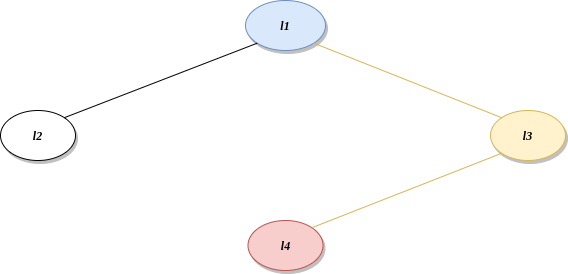
\includegraphics[scale=0.5]{figures/agent_example.png}
    \caption{Ejemplo del problema del agente. Su posición inicial es la ubicación
             $l1$ en azul queriendo llegar a la posición $l4$ marcada con rojo.}
    \label{fig:agent_example}
\end{figure}

\section{Representaciones STRIPS}

Un dato de entrada necesario para cualquier algoritmo de planificación es una
descripción del problema a ser resuelto. En la práctica, es usualmente imposible
incluir una enumeración explícita de todos los estados y transiciones que se
pueden realizar en el dominio a partir de una tarea STRIPS. Por lo tanto, es
necesario una representación que permita computarlas dinámicamente.

Consideremos el problema del ejemplo anterior donde se tiene el agente $a_1$
pero esta vez $n$ ubicaciones. Para este caso, se va a necesitar $n$ símbolos
proposicionales $p_i$ tal que representen la acción ``El agente $a_1$ está en la
ubicación $i$``. Si en lugar de un solo agente hubiese una cantidad $m$ de
ellos. Se necesitarían $n \times m$ símbolos para modelar esta característica de
la tarea. Una forma más compacta de representar esta propiedad es por medio de
un predicado de la forma $at(x, l)$ donde $x$ denota a un agente, y $l$ su
ubicación, siendo mucho más flexible debido a su naturaleza esquemática.

De manera similar, si se quisiera modelar una acción de cambio de posición,
haría falta describir una por cada agente y par de ubicaciones obteniendo un
total de $m \times n \times n$ instancias. Una mejor alternativa es representar
esta transformación por medio de un esquema de acción de la forma $move(x, l,
l')$ donde $x$ representa al agente, $l$ la ubicación actual, y $l'$ la ubicación
a la cual moverse.

De esta manera resulta más adecuado para la especificación utilizar predicados y
esquemas de acción en lugar de símbolos proposicionales. Esto lleva a las
siguientes definiciones:

\begin{mydef}
    Una especificación de una tarea STRIPS es una 6-upla $(\mathcal{P},
    \mathcal{A}, \Sigma^{C}, \Sigma^{O}, I, G)$  donde $\mathcal{P}$ es un
    conjunto de predicados, $\mathcal{A}$ es un conjunto de esquemas de acción,
    $\Sigma^{C}$ es un conjunto de símbolos constantes, $\Sigma^{O}$ es un conjunto de 
    variables, $I \subseteq 2^{\mathcal{P}}$ es el estado inicial, y $G \subseteq 2^{\mathcal{P}}$
    es la meta.
\end{mydef}

\begin{mydef}
    Sea $(\mathcal{P}, \mathcal{A}, \Sigma^{C}, \Sigma^{O}, I, G)$ una
    especificación de una tarea STRIPS.

    \begin{itemize}
        \item Un esquema de acción es una 3-upla $a[X] = (pre(a), add(a),
        del(a))$ donde cada elemento es subconjunto de $\mathcal{P}$, y $X$ es el
        conjunto de variables que ocurren en $pre(a) \cup add(a) \cup del(a)$ y
        que son parte de $\Sigma^{O}$.
        \item Un predicado es un símbolo atómico de $\mathcal{P}$ de la forma
        $p[X]$ con $X$ un conjunto de variables que ocurren en su interfaz y
        que son parte de $\Sigma^{O}$.
    \end{itemize}
\end{mydef}

Para la tarea STRIPS del problema del agente una primera especificación podría ser definida de la siguiente manera:

\begin{align*}
    \mathcal{P} = \{&at(x, l)\} \\
    \mathcal{A} = \{&move(x, l, l')\} \\
    \Sigma^{C} = \{&a_1, l_1, l_2, l_3, l_4\} \\
    \Sigma^{O} = \{&x, l, l'\} \\
    I = \{&at(a_1, l_1)\} \\
    G = \{&at(a_1, l_4)\}
\end{align*}
\begin{align*}
    move(x, l, l') &= (pre(move), add(move), del(move)) \\
                   &= (\{at(x, l)\}, \{at(x, l')\},\{at(x, l)\})
\end{align*}

Una diferencia importante es que ahora $move(x, l, l')$ es un esquema de acción donde $x$, $l$, $l'$ son variables libres pertenecientes a $\Sigma^{O}$. De esta manera, las variables se hicieron parte de la especificación, logrando expresar predicados y acciones de manera esquemática.

Por otro lado, está especificación de la tarea STRIPS, instancia más acciones que las del problema anterior, en particular, $move(a_1, l_2, l_4)$ está especificada como un movimiento posible. Por lo tanto, para representar exactamente el grafo de la figura \ref{fig:agent_example} es necesario agregar a la especificación un predicado extra, $is\_connected(l, l')$, que represente la existencia de un camino entre $l$ y $l'$. Luego, la estructura del grafo de la figura \ref{fig:agent_example} debe incluirse en el estado inicial. Además, el esquema de acción $move(x, l, l')$ debe poder aplicarse en un estado siempre y cuando exista un camino entre $l$ y $l'$.

\begin{align*}
    \mathcal{P} = \{&at(x, l)\} \\
    \mathcal{A} = \{&move(x, l, l')\} \\
    \Sigma^{C} = \{&a_1, l_1, l_2, l_3, l_4\} \\
    \Sigma^{O} = \{&x, l, l'\} \\
    I = \{& at(a_1, l_1), \\
          & is\_connected(l_1, l_2), is\_connected(l_2, l_1), \\
          & is\_connected(l_1, l_3), is\_connected(l_3, l_1), \\
          & is\_connected(l_3, l_4), is\_connected(l_4, l_3)\} \\
    G = \{& at(a_1, l_4), \\
          & is\_connected(l_1, l_2), is\_connected(l_2, l_1), \\
          & is\_connected(l_1, l_3), is\_connected(l_3, l_1), \\
          & is\_connected(l_3, l_4), is\_connected(l_4, l_3)\}
\end{align*}
\begin{align*}
    move(x, l, l') &= (pre(move), add(move), del(move)) \\
                   &= (\{at(x, l), is\_connected(l, l')\}, \{at(x, l')\},\{at(x, l)\})
\end{align*}

Un detalle de esta especificación es que es no tipada. Por ejemplo $move(a_1, a_1, a_1)$ es una acción instanciable. Lo cual deja en claro la necesidad de una representación de tareas que preserve los tipos de los esquemas de acción y predicados, y así evitar preprocesar acciones innecesarias durante el proceso de grounding.

Por último, un plan que resuelve la tarea STRIPS instanciada, es a su vez un plan para la especificación siendo está relación la que permite vincular ambas representaciones.

\section{El lenguaje PDDL}

Para especificar una tarea de planning a una computadora se necesita definir un
lenguaje que permita al usuario definir cada una de sus componentes. Para dar
respuesta a esta necesidad surge el \emph{Planning Domain Specification
Language} (PDDL), Propuesta para la competencia de planning
AIPS-98 \citep{McDermott1998} siendo el lenguaje de especificación de dominios y problemas de planning más usado dentro
de la comunidad de planning.

Una especificación en PDDL consiste de dos archivos, la definición del dominio,
donde se aclaran los predicados y esquemas de acción disponibles; y la
definición de la tarea donde se mencionan los objetos concretos a modelar, el
estado inicial, y la meta. Esta separación resulta importante, ya que diferentes
tareas de un mismo dominio comparten una estructura común.

Los listing \ref{lst:agent-domain} y \ref{lst:agent-task} muestran los archivos
de dominio y tarea del ejemplo del agente escrita en PDDL.

\begin{lstlisting}[
    float=!htb,
    caption={Dominio Agent en PDDL.},
    label={lst:agent-domain},
    language=PDDL]
  (
    define (domain AGENT-DOMAIN)

    (:requirements :strips :typing)

    (:types AGENT LOCATION)

    (:predicates (at ?x - AGENT ?l - LOCATION)
                 (is_connected ?l - LOCATION ?l' - LOCATION)
    )

    (:action move
        :parameters (?x - AGENT ?s - LOCATION ?d - LOCATION)
        :precondition (and (at ?x ?s) (is_connected ?l ?l'))
        :effect (and (not (at ?x ?s)) (at ?x ?d))
    )
  )
\end{lstlisting}

\begin{lstlisting}[
    float=!htb,
    caption={Ejemplo de una tarea del dominio Agent en PDDL.},
    label={lst:agent-task},
    language=PDDL]

  (
    define (problem AGENT-TASK)

    (:domain AGENT-DOMAIN)

    (:objects a1 - AGENT l1 l2 l3 l4 - LOCATION)

    (:init at(a1, l1)
           (is_connected l1 l2)
           (is_connected l2 l1)
           (is_connected l1 l3)
           (is_connected l3 l1)
           (is_connected l3 l4)
           (is_connected l4 l3)
           (is_connected l1 l2)
           (is_connected l2 l1)
           (is_connected l1 l3)
           (is_connected l3 l1)
           (is_connected l3 l4)
           (is_connected l4 l3)
    )
    
    (:goal (and 
           (at a1 l4)
           (is_connected l1 l2)
           (is_connected l2 l1)
           (is_connected l1 l3)
           (is_connected l3 l1)
           (is_connected l3 l4)
           (is_connected l4 l3)
           (is_connected l1 l2)
           (is_connected l2 l1)
           (is_connected l1 l3)
           (is_connected l3 l1)
           (is_connected l3 l4)
           (is_connected l4 l3)
           )
    )
  )
\end{lstlisting}

Observar que tanto los predicados como las acciones están parametrizados con variables de un cierto
tipo. Por ejemplo para el predicato $at(x, y)$, $x$ es de tipo \emph{AGENT} e $y$ del tipo \emph{LOCATION} ambos previamente listados en la linea 6 del listing \ref{lst:agent-domain}. Luego en la linea 7 del listing \ref{lst:agent-task} se especifican todos los objetos disponibles y el tipo al cual corresponden.

\section{Relajación por deletes}

El problema de decidir si una tarea de planning STRIPS tiene un plan es
PSPACE-completo. Es por eso que las implementaciones que lo resuelven son a partir de algoritmos de búsqueda de orden exponencial. El planificador instancia un problema y realiza una búsqueda exhaustiva guiada por medio de una función heurística definida a partir de \emph{planes relajados}. Un plan relajado es un plan en un dominio donde a todas las acciones se les eliminaron los efectos negativos. Es decir su lista $del$. Si bien no es exactamente el dominio sobre el cual se desea resolver la tarea original, brinda información relevante para hallar una solución. En particular, si los planes relajados permiten guiar la búsqueda para encontrar un plan de la tarea, entonces también podría ser usado para guiar el proceso de grounding.

Los planes relajados son secuencias de acciones cuyos efectos negativos son eliminados, son aplicables en el estado inicial, y su estado resultante contiene a la meta. Esto proviene de la \emph{relajación por deletes}, una simplificación de la tarea de planning que consiste en
eliminar los efectos negativos de las acciones. Esta
relajación es ampliamente utilizada en planning y su importancia subyace en la
siguiente propiedad: en la \emph{relajación por deletes} si un \emph{fact} $p$ se
vuelve verdadero en un estado $s$, entonces para toda secuencia de acciones $\vec{a} \in A^{*}$ aplicables en $s$, el estado resultante también hará verdadero $p$. Por ejemplo, en el
problema del agente, si este se desplazó por varias ubicaciones, tendríamos que
se encuentra en más de un lugar al mismo tiempo ya que la proposición que
indicaba su ubicación anterior no puede ser borrada. Esta propiedad es la que permite que computar un plan en el dominio relajado sea polinomial en comparación al dominio original.

\begin{mydef}
    Sea $\Pi = (F, A, I, G)$ una tarea STRIPS.
    \begin{itemize}
        \item Sea $a \in A$, definimos a la acción relajada por delete $a^{+}$
        dada por $pre(a^{+}) = pre(a)$, $add(a^{+}) = add(a)$, y $del(a^{+}) =
        \emptyset$.

        \item Denotaremos con $A^{+} = \{a^{+} : a \in A\}$ al conjunto de
        acciones relajadas por delete.

        \item Para una secuencia de acciónes $\vec{a}$ denotaremos con
        $\vec{a}^{+}$ a la secuencia de acciones relajadas por delete.

        \item Denotaremos con $\Pi^{+} = (F, A^{+}, I, G)$ a la tarea STRIPS
        relajada por deletes.

        \item Un plan relajado para $\Pi$ es un plan para $\Pi^{+}$.
    \end{itemize}
\end{mydef}

Claramente es una modelización no realista, no obstante, relajar una tarea STRIPS provee información importante sobre la tarea original, en particular:

\begin{lemma}
\label{lit:delete_relaxed_property}
Sea $\Pi = (F, A, I, G)$ Una tarea STRIPS
\begin{itemize}
    \item Si una secuencia de acciones $\vec{a}$ es un plan de $\Pi$, entonces $\vec{a}^{+}$ es un plan relajado de $\Pi$.
    \item Si no existe un plan para $\Pi^{+}$ entonces no existe un plan para $\Pi$.
\end{itemize}
\end{lemma}

Estas propiedades serán muy relevantes al introducir los algoritmos de grounding en las secciones \ref{lit:relaxed_grounding}, y \ref{lit:heuristic_grounding}. La primera de ellas nos dice que un plan de una tarea STRIPS, es a la vez un plan de la tarea relajada. No obstante el reciproco no se cumple. Por lo general, un plan en la tarea relajada no es un plan de la tarea original. La segunda de ellas menciona que si no existe un plan para la tarea relajada, entonces no hay un plan para la tarea original. Esto también es importante ya que todo plan en la tarea relajada puede encontrarse con solo instanciar aquellas acciones que sean alcanzables. Si no se encuentra un plan de la tarea relajada para ese conjunto de acciones, entonces sabremos que no existirá solución en la tarea original.

\section{Proceso de grounding}
\label{lit:relaxed_grounding}

Dada una especificación de una tarea STRIPS $(\mathcal{P}, \mathcal{A},
\Sigma^{C}, \Sigma^{O}, I, G)$ se puede obtener su correspondiente tarea $\Pi =
(F, A, I, G)$ recolectando todas las instancias posibles de predicados en
$\mathcal{P}$ y esquemas de acción de $\mathcal{A}$ con objetos de $\Sigma^{C}$.
Es decir, $F$ contiene un \emph{fact} por cada posible asignación de objetos a
los argumentos de cada predicado $P[X] \in \mathcal{P}$, y $A$ contiene una
acción por cada posible asignación de objetos a los argumentos de cada esquema
de acción $a[X] \in \mathcal{A}$. Este proceso se conoce como \emph{grounding
cartesiano}.

No obstante, en la práctica los planificadores no instancian todas las posibles
acciones y proposiciones, sino aquellas que son alcanzables relajadamente desde
el estado inicial debido al lemma \ref{lit:delete_relaxed_property}. 

Este proceso de grounding es el implementado por \emph{Fast Downward} \citep{Helmert-2011}, el sistema de planning clásico basado en búsqueda heúristica más popular por la comunidad debido a su excelente desempeño en benchmarks, competencias internacionales de planning, e implementaciones eficientes de algoritmos genéricos de búsqueda. Estas implementaciones son altamente configurables por Fast Downward permitiendo ajustarse a distintos dominios de planning. Su popularidad y versatilidad fue la motivación que nos llevó a utilizarlo en esta tesis en comparación a otros sistemas.

\begin{mydef}
    Sea $\Pi = (F, A, I, G)$ una tarea STRIPS.    
    \begin{itemize}
        \item Un estado $s \subseteq F$ es alcanzable en $\Pi$ si existe una
        secuencia $\vec{a}$ en $A^{*}$ tal que $I \xrightarrow{\vec{a}} s$.
    
        \item Un proposición $p \in F$ es alcanzable en $\Pi$ si existe un estado
        $s$ alcanzable en $\Pi$ tal que $p \in s$.

        \item Una acción $a \in A$ es alcanzable en $\Pi$ si existe una estado $s$
        alcanzable en $\Pi$ tal que $a$ es aplicable en $s$.

        \item Un proposición $p \in F$ es alcanzable relajadamente en $\Pi$ si
        $p$ es alcanzable en $\Pi^{+}$.

        \item Una acción $a \in A$ es alcanzable relajadamente en $\Pi$ si
        $a^{+}$ es alcanzable en $\Pi^{+}$.
    \end{itemize}
\end{mydef}


\begin{algorithm}
    \caption{Grounding por alcanzabilidad
    relajada}\label{alg:grounding_delete_relaxed}
    \begin{algorithmic}[1]
    \Require Especificación de una tarea STRIPS $(\mathcal{P}, \mathcal{A},
    \Sigma^{C}, \Sigma^{O}, I, G)$
    \Ensure Tarea STRIPS $(F, A, I, G)$ 
    \State $q \gets Queue(I)$
    \State $F \gets \emptyset$
    \State $A \gets \emptyset$
    \While{$ \lnot q.empty()$}
    \State $e \gets q.pop()$
    \If{$e.isFact()$}
        \State $F \gets F \cup \{e\}$
        \For{$a \notin A \land pre(a) \subseteq F$}
            \State $q.insert(a)$
        \EndFor
    \Else
        \State $A \gets A \cup \{e\}$
        \For{$f \notin F \land f \in add(e)$}
            \State $q.insert(f)$
        \EndFor
    \EndIf
    \EndWhile
    \State \Return $(F, A, I, G)$
    \end{algorithmic}
\end{algorithm}

El algoritmo \ref{alg:grounding_delete_relaxed} implementado por Fast Downward
parte de una cola $q$ que almacena todos los símbolos proposicionales del estado
inicial. Luego la cola $q$ almacena elementos a preprocesar que pueden ser tanto facts como acciones. A partir de allí, se remueve elemento a elemento de $q$ consultando si
es un fact o una acción.

En el caso de encontrarse con un fact, se lo instancia y se agregan a $q$ todas
las acciones aplicables (aún no procesadas) a partir de las proposiciones
groundeadas hasta el momento. Caso contrario, se obtiene una acción que también
se instancia y se agregan a $q$ todas las proposiciones (aún no procesadas) que
ocurren positivamente en su efecto, es decir, su lista $add$.

Este procedimiento se repite hasta que la cola se encuentre vacía, obteniendo de esta manera todas las acciones y facts alcanzables relajadamente.

\section{Grounding heurístico}
\label{lit:heuristic_grounding}

Mencionamos que un plan de una tarea es también un plan relajado de la misma.
Sin embargo, el reciproco no se cumple. Es más, un hecho o una acción que es
relajadamente alcanzable, puede no ser alcanzable en la tarea original o ser
irrelevante al no pertenecer a ningún plan que la resuelva. Es justamente esta
pérdida de información la que origina que computar en el mundo relajado sea
polinomial. Es aquí donde surge el foco de este trabajo donde se intentará
predecir cual de estos hechos y acciones son verdaderamente relevantes para
alcanzar la meta, priorizando su instanciación por sobre el resto.

\begin{algorithm}
    \caption{Grounding heurístico}\label{alg:grounding-heuristico}
    \begin{algorithmic}[1]
    \Require Especificación de una tarea STRIPS $(\mathcal{P}, \mathcal{A}, \Sigma^{C}, \Sigma^{O}, I, G)$. Número máximo de instanciaciones permitidas $N$
    \Ensure Tarea STRIPS $(F, A, I, G)$
    \State $q \gets PriorityQueue(I)$
    \State $F \gets \emptyset$
    \State $A \gets \emptyset$
    \While{$ \lnot (q.empty() \lor G \subseteq F) \land |A| \leq N$}    
    \If{$q.containsFact()$}
        \State $f \gets q.popFact()$
        \State $F \gets F \cup \{f\}$
        \For{$a \notin A \land pre(a) \subseteq F$}
            \State $q.insert(a)$
        \EndFor
    \Else
        \State $a \gets q.popHighPriorityAction()$
        \State $A \gets A \cup \{a\}$
        \For{$f \notin F \land f \in add(a)$}
            \State $q.insert(f)$
        \EndFor
    \EndIf
    \EndWhile
    \State \Return $(F, A, I, G)$
    \end{algorithmic}
\end{algorithm}

El algoritmo de grounding heurístico que presentaremos es el mismo que se
desarrolló en \citep{Gnad_Torralba_Dominguez_Areces_Bustos_2019} y está basado
en el que se mostró en la sección anterior. Las principales diferencias son el
criterio de parada, donde se procesan no más de $N$ acciones, y el orden en que
lo hacen, según su nivel de relevancia. Debido a que el algoritmo puede
terminar antes de que la cola se vacíe, se está obligado a procesar la totalidad
de los facts existentes en la cola antes de considerar una siguiente acción. Esto garantiza
que todos los facts que se encuentran en los efectos de las acciones ya
procesadas están en $F$, siendo el algoritmo \emph{fact consistente}.

\begin{mydef}
    Sean $F$ y $A$ el conjunto de facts y acciones retornados por un algoritmo
    de grounding. Decimos que este es fact consistente si para todo $a \in A$ se
    cumple que, si $p \in pre(a) \cup add(a) \cup del(a)$ entonces $p \in F$.
\end{mydef}

En grounding heurístico, el algoritmo puede detenerse mucho antes según el
parámetro $N$ que indica la cantidad de instancias que puede realizar el proceso
sin que los recursos de tiempo y memoria se vean comprometidos. Por lo general,
muchas de los problemas de planning requieren planes cortos del orden de a lo
sumo cientos de acciones en comparación a posiblemente millones de operadores
groundeados.

Es importante mencionar que este algoritmo es \emph{correcto}, si hallamos un
plan de la tarea obtenida por grounding heurístico, entonces ese mismo plan lo
es para la tarea obtenida por grounding total. No obstante, no es
\emph{completo}, una tarea obtenida por grounding heurístico tiene solución si y
sólo si las acciones correspondientes de al menos un plan (de la tarea obtenida
por grounding total) fueron procesadas.

Por último, algo a considerar es el remplazo de la cola del Algoritmo
\ref{alg:grounding-heuristico}, por una cola de prioridades que asigna a las
acciones un nivel de relevancia por la cual son ordenadas. La relevancia de una
acción está directamente relacionada con la probabilidad de que esta pertenezca
a un plan de la tarea. Notar que una estimación ideal sería una probabilidad de
1 para las acciones que ocurren en algún plan de la tarea y 0 para las
restantes. Pero computar esto es tan difı́cil como obtener una solución
y sabemos que es PSPACE-completo. Es por eso que para estimar la relevancia se
utilizaron técnicas de aprendizaje automático y serán el foco del siguiente
capítulo.

    \chapter{Aprendizaje automático}
\label{ch:lit_ml}

En este capítulo se profundizará en el área de \emph{aprendizaje automático}
abarcando la representación de palabras y oraciones dadas por codificaciones del
tipo one-hot, word embeddings, conceptos de aprendizaje supervisado y no
supervisado, modelos de clasificación, y métricas. Este capítulo se baso en mayor parte del contenido en \citep{Bishop-2006}, y \citep{Tianqi-2016} para la explicación de conceptos de aprendizaje supervisado, y  \citep{Bojanowski-Grave-Joulin-Mikolov-2016, bojanowski-2017, Mikolov-2013} para representación de palabras.

\section{Orígenes y evolución}

El aprendizaje automático es el campo de la inteligencia artificial que busca
desarrollar programas que mejoren en base a la experiencia. Estos métodos
difieren del típico paradigma de implementación donde en lugar de ser
``programado`` es ``entrenado``. Tal entrenamiento consiste en disponerle al
algoritmo información en forma de ejemplos con el fin de reconocer patrones
estadísticos y eventualmente determinar reglas que sirvan para automatizar una
tarea.

Por moderno que pueda parecer este campo, tuvo sus comienzos en los años 50 a
partir del famoso \emph{Test de Turing}, una máquina cuyo objetivo era engañar a
un humano haciéndole creer que se encontraba delante de otra persona en lugar de
un ordenador, llegando  a la conclusión de que los computadores de propósito
general, podrían ser capaces de aprender y ser de alguna manera originales.
\footnote{\url{https://www.turing.org.uk/scrapbook/test.html}}

En los últimos años varias aplicaciones se han beneficiado de esta área, desde
programas relacionados con la detección fraudulenta de transacciones con tarjeta
de crédito \citep{Fang-2021}, sistemas de recomendación que guían usuarios en un servicio de
acuerdo a sus preferencias \citep{Burke-2007}, o incluso vehículos que se manejan sin necesidad de
la intervención del conductor \citep{Sorin-2019}. Al mismo tiempo, una importante cantidad de
avances teóricos y algorítmicos se fueron realizando formando las bases de este
campo.

Aún con estos increíbles logros, no se conoce aún como crear computadoras que
aprendan al nivel que las personas lo hacen. No obstante, se han desarrollado
algoritmos que se han aproximado a este objetivo siendo efectivos para varios
tipos de problemas.

\section{Aprendizaje supervisado}

El aprendizaje supervisado es una subárea del aprendizaje automático cuyo
objetivo es deducir un modelo a partir de datos anotados que permita mapear
ejemplos no vistos previamente. Esta información está compuesta por un conjunto
de ejemplares y sus correspondientes etiquetas, en ocasiones dada por un
anotador humano, la cual indica el resultado esperado del modelo a partir del dato como
entrada. Las etiquetas pueden ser categóricas o continuas determinando un
problema de clasificación o regresión. Algunas tareas más frecuentes de
clasificación son la categorización de documentos, reconocimiento de lenguaje
ofensivo, o análisis de sentimiento. Mientras que para regresión, lo son las
estimaciones de precios de artículos, objetos, o viviendas.

El resultado de ejecutar un algoritmo de machine learning supervisado se puede
expresar como una función $f(\vect{x})$ que recibe un ejemplar $\vect{x}$ como
entrada y genera un valor $y$ de salida codificado de la misma manera
que las etiquetas. Las muestras utilizadas para ajustar $f$ están dadas por
pares (vector, etiqueta) $\{(\vect{x}_1, y_1), ..., (\vect{x}_n, y_n)\}$
conformando el \emph{conjunto de entrenamiento}.

La forma precisa de $f$ es determinada durante la fase de entrenamiento. Una vez
transcurrida, se puede estimar la identidad de nuevos datos etiquetados
pertenecientes al \emph{conjunto de test} con el fin de evaluar la performance
del modelo. En el caso que la predicción se aproxime a la esperada para estas
nuevas entradas, entonces el modelo habría logrado generalizar la tarea.

Sin embargo, los modelos de aprendizaje supervisado están limitados por la
disponibilidad de las anotaciones y la dificultad para obtenerlas.
Algunas tareas son relativamente sencillas de etiquetar por cualquier
persona, (e.g. como determinar si en una foto aparece un gato), mientras que en
otros puede llegar a requerir humanos que sean expertos de dominio (e.g.
abogados, médicos, lingüistas, etc).

\section{Aprendizaje no supervisado}

En contraste al método anterior, el aprendizaje no supervisado consiste en
descubrir automáticamente patrones sobre los datos de entrenamiento que permitan
explicarlos sin depender de datos de anotados. Es considerada como parte del
área del análisis y exploración. Es por eso que no pueden ser evaluados
basándose en exactitud o precisión, si no más bien en la cantidad de información
que podamos extraer de los datos a partir del uso de estas técnicas. Algo a
considerar es la facilidad para disponer de estos datos (en comparación a los no
supervisados) al no requerir ningún tipo de supervisión humana.

\section{Algoritmos de clasificación}
\label{lit:algorithms}

Comenzaremos estudiando algunos métodos de aprendizaje supervisado sin preocuparnos
inicialmente por la manera en que los ejemplares están codificados con excepción de las etiquetas. Es decir para un conjunto de entrenamiento $\{(\vect{x}_1, y_1), ..., (\vect{x}_n, y_n)\}$ la codificación de los $\vect{x}_i's$ será irrelevante por el momento. La únicas restricciones que se pedirán es que sean vectores numéricos. Los $y_i's$ aparte de ser
numérico debe ser categórico dado que trataremos con algoritmos de clasificación.

El objetivo principal de un clasificador es aproximar una función no conocida
$f$ a partir de un modelo $h: \mathbb{R}^D \rightarrow \{c_1,.., c_k\}$ la cual
mapea ejemplos de entrada a una categoría $c_j$. En particular, nos enfocaremos
en clasificadores binarios $k = 2$ que fueron los utilizados para la realización
de este trabajo.

\subsection{Modelos lineales}

La forma más sencilla de representar un función que discrimine datos de entrada
en dos clases es a partir de una función lineal que dependa de estos datos:

\begin{align}
    h_{\vect{w}, w_0}\left( \vect{x} \right) &= \vect{w}^{\top} \vect{x} + w_0  \label{eq:linear_w_bias}\\
                                           &= \sum_{j = 1 }^{D} w_j x_j + w_0 \label{eq:linear_wo_bias}
\end{align}

Donde $\vect{w}$ es llamado el \emph{vector de pesos}, y $w_0$ es el
\emph{sesgo}. Ambos son parámetros de la función $h$ y son los que se buscan
ajustar para lograr separar el conjunto de datos donde $\vect{x}$ es uno de tales
ejemplos. Las dimensiones de los vectores $\vect{x}$, y $\vect{w}$ son ambas $(D
\times 1)$ a diferencia del sesgo que es un escalar. La expresión
$\vect{w}^{\top} \vect{x}$ es el producto interno entre $\vect{w}$ y $\vect{x}$.
Por lo que el resultado de $\vect{w}^{\top} \vect{x} + b$ es también un escalar.
Dado que nos interesa asignar a $\vect{x}$ una categoría, se debe decidir a cual
pertenece en base al resultado obtenido por el producto interno. Es por eso que
surge la necesidad de agregar una nueva operación que discrimine un valor de
entrada en una clase. Para ello definimos una \emph{función de decisión} $d: \mathbb{R} \rightarrow
\{c_1, c_2\}$ tal que mapea valores a una clase $c_1$, o $c_2$.

Una posible función de decisión podría estar definida como $d(t) = c_1$ si $t
\geq 0$, $d(t) = c_2$ caso contrario. Por lo tanto la frontera de decisión queda
definida por la relación $h_{\vect{w}, w_0}\left( \vect{x} \right) = 0$ y
corresponde a un hiperplano de ($D-1$ dimensiones) en uno de $D$ dimensiones. El
sesgo $w_0$ desplaza el hiperplano del origen coordenados de $D$. Un ejemplo de pares de puntos separados por un hiperplano (en este caso una recta) se muestra en la figura \ref{fig:linear_model_boundary}.

Algunas veces es conveniente usar una notación más compacta en la que
introducimos una ``inocente`` componente de entrada más $x_0 = 1$ al vector
$\vect{x}$ para luego definir $\vect{w}' = (w_0, \vect{w})$ y $\vect{x}' = (x_0,
\vect{x})$. Luego las ecuaciones \ref{eq:linear_w_bias} y \ref{eq:linear_wo_bias}
se pueden expresar como:

\begin{figure}
    \centering
    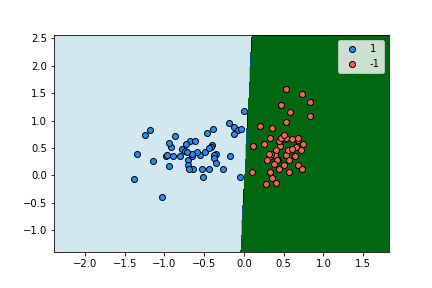
\includegraphics[scale=0.5]{figures/decision_boundary.png}
    \caption{Frontera de decisión de un modelo lineal separando los puntos que tienen etiqueta $c_1$ = 1 y $c_2$ = -1}.
    \label{fig:linear_model_boundary}
\end{figure}

\begin{align}
    h_{\vect{w'}}\left( \vect{x'} \right) &= \vect{w'}^{\top} \vect{x'}\\
                                           &= \sum_{j = 0 }^{D} w_j x_j
\end{align}

Ahora la frontera de decisión corresponde a un hiperplano de dimensión $D$ que
pasa por el origen del espacio $D + 1$ dimensional. A partir de ahora, cada vez
que se omita el sesgo estaremos utilizando esta notación.

\subsection{Modelos probabilísticos}
\label{subch:prob_models}

En el capítulo \ref{ch:lit_planning} mencionamos que el objetivo de usar un algoritmo de aprendizaje
automático es determinar una función que modele la probabilidad
de que una acción sea relevante para encontrar un plan de una tarea STRIPS. Sin
embargo, desconocemos aún de que manera se obtienen estas probabilidades, es por
eso que el foco de esta sección es indagar sobre los modelos probabilísticos.

En estos modelos se busca modelar la densidad condicional $p(c_k | \vect{x})$ que
representa la probabilidad de la clase $c_k$ dado $\vect{x}$. El inconveniente con
esto es que cada condicionamiento define una densidad probabilística. Por lo que
se tendría una por cada posible ejemplar $\vect{x}$ resultando intratable de
modelar. No obstante, si se considera el condicionamiento $p(\vect{x} | c_k)$
solo es necesario modelar una cantidad pequeña de clases, en especial para un
clasificador binario. Para nuestra suerte $p(c_k | \vect{x})$, está relacionado
con $p(\vect{x} | c_k)$ por la \emph{regla de Bayes}.

\begin{align}
    p\left( c_1 | \vect{x} \right) &= \frac{p\left( \vect{x} | c_1 \right)p(c_1)}{
                                            p\left( \vect{x} | c_1 \right) p(c_1) + 
                                            p\left( \vect{x} | c_2 \right)p(c_2)} \\
                                   &= \frac{1}{1 + \exp\left( -a \right)} \\
                                   &= \sigma(a)
\end{align}

Donde definimos $a = \ln \frac{p\left( \vect{x} | c_1 \right) p\left( c_1
\right)}{p\left( \vect{x} | c_2 \right) p\left( c_2 \right)}$. La función
$\sigma(a)$ es conocida como la función \emph{sigmoide} y juega un importante
rol en muchos algoritmos de clasificación por su propiedad de simetría
$\sigma(-a) = 1 - \sigma(a)$, el significado de su inversa $a = \ln \left(
\frac{\sigma}{1 - \sigma} \right)$ que representa el logaritmo del radio de las
probabilidades de las clases $c_1$ y $c_2$, y la capacidad de mapear el eje real
en un intervalo finito.

Se puede generalizar esta ecuación para el caso $k > 2$ de la siguiente manera:

\begin{align}
    p\left( c_k | \vect{x} \right) &= \frac{p\left( \vect{x} | c_k \right)p(c_k)}{
                                                \sum_{j=1}^{k} p\left( \vect{x} |
                                                c_j \right) p(c_j) } \\
                                       &= \frac{\exp\left( a_k \right)}{\sum_{j=1}^{k} a_j} \\
\end{align}

Donde $a_k = \ln p\left( \vect{x} | c_k \right) p\left( c_k \right)$. La función
$\frac{\exp\left( a_k \right)}{\sum_{j=1}^{k} a_j}$ es conocida como la función
\emph{softmax} ya que es una versión suavizada de la función $max$ en el sentido de
si $a_k >> a_j$ para todo $j \neq k$ entonces $p(c_k | \vect{x}) \approx 1$ y
$p(c_j | \vect{x} \approx 0)$.

\subsection{Función de costo}

Varios de los métodos de machine learning existentes no pueden obtener los pesos
$W$ de manera analítica. Es por eso que se hacen uso de métodos iterativos en
base a una \emph{función de costo} que mide la precisión de su predicción en
comparación con la etiqueta. Si tenemos ejemplos de entrenamiento
$\{(\vect{x}_{1}, y_{1}), ..., (\vect{x}_{n}, y_{n})\}$ podemos definir la
función de costo en base a cada ejemplar $i$.

Un ejemplo clásico de función de costo es el error cuadrático medio:

\begin{align}
    J(\vect{w}) = \frac{1}{2n} \sum_{i=1}^{n}\left( h_{\vect{w}}\left( \vect{x}_{i}\right) - y_i \right)
\end{align}

Por lo tanto, al minimizar $J$ se estará reduciendo el error de estimación de $h$
obteniendo que $h_{\vect{w}}\left( \vect{x}_{i} \right) \approx f(\vect{x}_{i})$. Para
lograr tal minimización, existe una técnica denominada \emph{descenso por el
gradiente}. la cual actualiza de manera iterativa el vector $\vect{w}$ logrando
la convergencia de la función de costo $J$ a un mínimo valor.

\subsection{Descenso por el gradiente}

Definimos $\vect{\Delta J\left( w \right)}$ al gradiente de $J$ en $\vect{w}$
como $\vect{\Delta J\left( \vect{w} \right)} = \left(\frac{\partial
J(\vect{w})}{\partial w_1}, ..., \frac{\partial J(\vect{w})}{\partial w_n}
\right)$, el vector de derivadas parciales. Este algoritmo empieza con una
inicialización aleatoria de $\vect{w}$ y calcula
$\vect{\Delta J\left( w \right)}$ por una cantidad de iteraciones. El negativo del gradiente indica la dirección de mayor descenso en el cual la función $J(\vect{w})$ disminuye. Por lo tanto si
al vector $\vect{w}$ se le suma el negativo del gradiente se estaría
dirigiéndolo en torno a un mínimo local de la función de costo. La magnitud del
desplazamiento vectorial en cada iteración está determinado por una constante
$\alpha$ conocida como la \emph{taza de aprendizaje}.

\begin{align} \label{eq:gradient_descent}
    \vect{w} \leftarrow \vect{w} - \alpha \vect{\Delta J\left( w \right)}
\end{align}

\begin{figure}
    \centering
    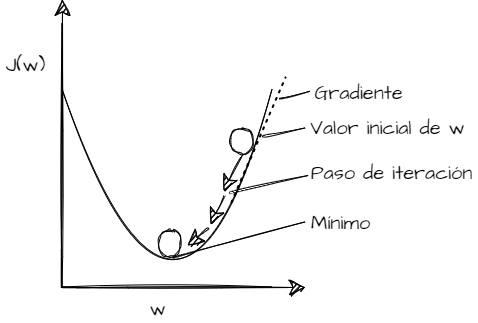
\includegraphics[scale=0.5]{figures/gradient_descent_plot.png}
    \caption{Intuición del método de descenso por el gradiente a partir del error cuadrático medio como función de costo $J$}
    \label{fig:gradient_descent}
\end{figure}

En cada iteración se realiza la operación de la ecuación actualizando
$\vect{w}$. Dado a que $\alpha$ > 0, el valor de cada parámetro en $\vect{w}$ disminuirá
y eventualmente la función de costo $J$ convergerá a su valor mínimo en $T$
iteraciones. Algo a notar es que la ecuación \ref{eq:gradient_descent}, al ser una operación vectorial, cada componente se actualiza simultáneamente. La figura \ref{fig:gradient_descent} muestra la intuición detrás de este método utilizando el error cuadrático medio como función de costo.

El método de descenso por el gradiente es también llamado el
optimizador de la función de costo. En la literatura hay varias variantes de
este método que llevan a optimizadores más complejos y eficientes, tales como
\emph{adam}, \emph{descenso por el gradiente estocástico}, entre otros.

\subsection{Sobreajuste (overfitting)}

Una vez optimizado la función de costo y haber encontrado los configuración de
$\vect{w}$ que minimiza la función de costo se pueden utilizar estos pesos
aprendidos para hacer predicciones de ejemplos no antes visto en el proceso de
entrenamiento. Sin embargo, algo que suele ocurrir al utilizar solamente la
función de costo para optimizar modelos de machine learning, es que tienden a
sobreajustar los datos de entrenamiento reduciendo su error pero obteniendo
malas predicciones en estos nuevos ejemplares. Por lo general, suele asociarse
con la magnitud de los coeficientes en $\vect{w}$ siendo muy alta para
estos casos. Otras razones de esto suele ser la dimensión de $\vect{w}$. En
cuanto mayor la cantidad de parámetros de ajuste, existen más chances de que el
modelo de machine learning memorice los datos de entrenamiento. Para solucionar esto se suele
recurrir a varias técnicas con el fin de obtener modelos sencillos pero que
logren generalizar la tarea que se está queriendo clasificar. Uno de ellos es
agregar a la función de costo un \emph{término de regularización} sobre las
componentes de $\vect{w}$ para lidiar el problema de su magnitud. Por ejemplo para
el error cuadrático medio:

\begin{align}
    J(\vect{w}) = \frac{1}{2n} \sum_{i=1}^{n}\left( h_{\vect{w}}\left( \vect{x}_{i}\right) - y \right) +
                  \frac{\lambda}{2} ||\vect{w}||^{2}
\end{align}

Donde $||\vect{w}||$ es la norma de \vect{w}, y $\lambda$ es la fuerza en que la regularización impacta.

Otros métodos para el control del overfitting dependen del método de
clasificación que se utilice, función de costo, parámetros de ajuste, entre
otros que iremos explicando a medida que avancemos con los modelos utilizados en
los experimentos.

\subsection{Regresión logística}

El primer modelo de clasificación que veremos es la \emph{regresión logistica}. Es un
clasificador binario que busca modelar la probabilidad a posterior de $c_1$ a
partir de una función sigmoide actuando sobre los vectores de
entrada:

\begin{align}
    p\left( c_1 | \vect{x} \right) = \sigma\left( \vect{w}^{\top} \vect{x} \right)
\end{align}

Luego $p\left( c_2 | \vect{x} \right) = 1 - p\left( c_1 | \vect{x} \right)$.
Para un espacio de características $\vect{x}$ de $D$ dimensiones este modelo
consta de $D$ parámetros para ajustar. En particular este método suele codificar
las etiquetas de las clases $c_1$ y $c_2$, como $0$ y $1$, ya que permite
algunas simplificaciones en la definición de su función de costo.

De esta manera podemos pensar la etiqueta $y$ como observaciones discretas de una
distribución bernoulli.

\begin{align}
    & p(y = 1 | \vect{x}) = h_{\vect{w}}(\vect{x}) \\
    & p(y = 0 | \vect{x}) = 1 - h_{\vect{w}}(\vect{x}) \\
    & p(y | \vect{x}) = (h_{\vect{w}}(\vect{x}))^{y}(1 - h_{\vect{w}}(\vect{x}))^{1 - y}
\end{align}

Luego los pesos $\vect{w}$ se obtienen a partir de un optimizador del tipo del
descenso por el gradiente minimizando la función de costo definida como:

\begin{align}
    J\left( \vect{w} \right) &= \sum_{i=1}^{n} p(y_{i} | \vect{x}_{i}) \\
                             &= -\sum_{i=1}^{n}
                                    y_{i}\log\left( h_{\vect{w}}\left( \vect{x}_{i} \right) \right) +
                                    (1 - y_{i})\log\left(1 - h_{\vect{w}}\left( \vect{x}_{i} \right) \right)
\end{align}

Algo a notar es que la función de costo se puede expresar como suma de penalizaciones
individuales:

\begin{align}
    J\left( \vect{w} \right) &= \sum_{i=1}^{n} \ell\left( h_{\vect{w}}\left( \vect{x}_{i}\right), y_{i}\right)
\end{align}

Donde $\ell$ es la penalización a nivel de ejemplo:

\begin{align}
    \ell\left( \vect{x}, y \right) =
    \begin{cases}
        - \log\left( h_{\vect{w}}\left( \vect{x} \right) \right) & y = 1 \\
        - \log\left(1 - h_{\vect{w}}\left( \vect{x} \right) \right) & y = 0
    \end{cases}
\end{align}

\begin{figure}
    \centering
    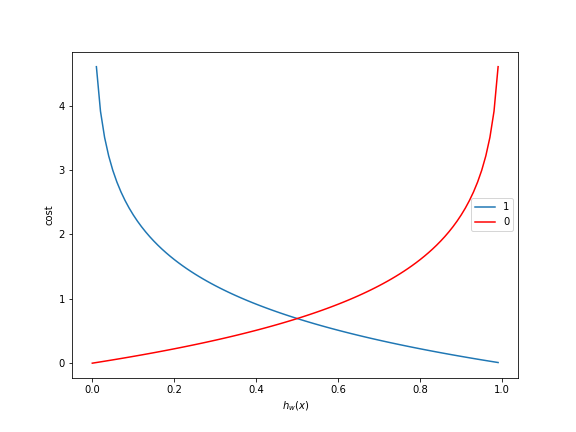
\includegraphics[scale=0.5]{figures/logistic_regression_loss.png}
    \caption{Gráfica de $h_{\vect{w}}(\vect{x})$ vs $\ell(\vect{x})$ separando por etiqueta}
    \label{fig:lgr_loss}
\end{figure}

Si analizamos la forma de $\ell$ para ambos casos podemos observar que, $J$
captura la intuición de que mayores errores en la predicción deben recibir
mayores penalizaciones.

Para el caso $y = 1$. La función de costo a nivel de
ejemplo es la curva que se marca en color azul de la figura \ref{fig:lgr_loss}. En ella se puede ver
que si $h_{\vect{w}}\left( \vect{x} \right) \rightarrow 0$ (la función de
predicción asigna a $\vect{x}$ una probabilidad cercana a $0$), entonces el
costo incrementa y por lo tanto $\ell(\vect{x}, y) \rightarrow \infty$. Si
$h_{\vect{x}}\left( \vect{x} \right) \rightarrow 1$, entonces el costo disminuye
y $\ell(\vect{x}, y) \rightarrow 0$. De manera similar ocurre para el caso $y =
0$ y la curva marcada en rojo.

\subsection{Redes neuronales}

Una red neuronal artificial es un modelo computacional que en los últimos
tiempos se ha convertido en el estado del arte y el enfoque más utilizado en la
mayoría de las áreas relacionadas al diseño e implementación de sistemas
predictivos. Estas áreas incluyen, entre otras el procesamiento del habla, la
visión por computadoras, el procesamiento del lenguaje natural y la toma de
decisiones y control en agentes situados.

El término surge bajo los intentos de definir un modelo matemático de una red
neuronal biológica \citep{McCulloch-Pitts-1990}. No obstante, enfocaremos nuestra atención en un tipo
especifico de red neuronal reconocida por su alto valor práctico, denominado
\emph{perceptrón multicapa}.

Las redes neuronales surgen de la necesidad de aprender la representación de los
datos cuya disposición en el espacio requieren de una modelización no lineal
mucho más compleja. Similar a un modelo lineal, las redes neuronales reciben un
vector de entrada $\vect{x}$ donde cada componente $x_i$ es ponderada mediante
una combinación lineal por el peso $w_i$ en $\vect{w}$. La única diferencia es que
al resultado se le aplica una función de transformación no lineal $g$ conocida
como \emph{función de activación}.

\begin{equation} \label{eq:nn}
    z_{\vect{w}}\left( \vect{x} \right) = g\left( \sum_{i=0}^{D} w_i x_i \right)
\end{equation}

Notar además que se puede pensar está red neuronal simple como un modelo de
regresión logística si la función de activación es la sigmoide, es decir, si $g
= \sigma$.

\subsection{Perceptrón multicapa}
\label{subch:multi_layer_perceptron}

Este modelo puede describirse como una serie de transformaciones similares a la
ecuación \ref{eq:nn}. Primero construimos $M + 1$ combinaciones lineales a partir de
las componentes del ejemplo de entrada $\vect{x} = (x_0, ..., x_D)$.

\begin{equation}
    a_j = \sum_{i = 0}^{D} w_{ji}^{(1)} x_{i}
\end{equation}

Donde $j = 0,..., M$. El supra-índice $(1)$ indica que los parámetros
correspondientes $w_{ji}^{(1)}$ están en la primera capa de la red. Luego cada
$a_j$ es transformado por una función de activación no lineal $g$.

\begin{figure}
    \centering
    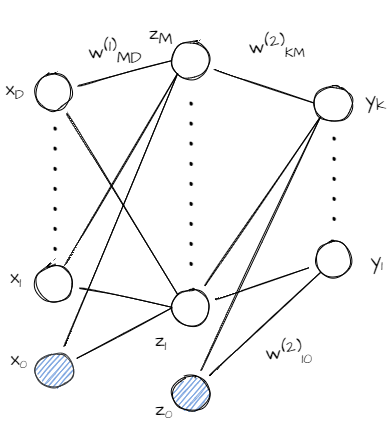
\includegraphics[scale=0.5]{figures/multilayer_perceptron.png}
    \caption{Perceptrón multicapa de una sola capa oculta}
    \label{fig:nn_multilayer_perceptron}
\end{figure}

\begin{equation}
    z_j = g(a_j)
\end{equation}

Estas cantidades corresponden a las salidas de cada neurona o unidad. Luego para
estos valores construimos nuevamente $K$ combinaciones lineales obteniendo $K$
neuronas de salida.

\begin{equation}
    a_k = \sum_{j=0}^{M} w_{kj}^{(2)}z_j
\end{equation}

Donde $k= 1,..., K$. Esta transformación corresponde con la segunda capa de la
red, como lo indica el supra-índice $(2)$. Finalmente los unidades de salidas
realizan su predicción $y_k$ activando los datos por última vez con otra función
de activación. Esta última depende de la codificación de la variable objetivo, y
si se está trabajando sobre un problema de regresión o clasificación. Para el
caso de regresión la función de activación de salida suele ser la función de
identidad, para clasificación binaria una sigmoide, y para multiclase una softmax.

\begin{equation}
    y_{k} = \sigma\left( a_k \right)
\end{equation}

Podemos combinar estas dos transiciones y dar una expresión del modelo completo
en función de $\vect{x}$ y $\vect{w}$.

\begin{equation}
    y_k(\vect{x}, \vect{w}) = \sigma\left(
                \sum_{j=0}^{M} w_{kj}^{(2)}
                    g\left( \sum_{i = 0}^{D} w_{ji}^{(1)} x_{i}
                \right)
            \right)
\end{equation}

Por lo tanto un modelo neuronal es simplemente una función no lineal que depende
de un ejemplo $\vect{x}$, que retorna un vector de salida $\vect{y}$, y que es
controlado por un vector de parámetros $\vect{w}$, donde las dimensiones de
estos vectores son $D + 1$, $K$, y $(D + 1 \times M + 1)$ respectivamente. Esta función
también puede representarse a partir de un gráfico de red como el que se vé en
la figura \ref{fig:nn_multilayer_perceptron} . El proceso de evaluar un ejemplo puede interpretarse como una
propagación hacia adelante (\emph{forward propagation} en inglés), que transmite
la información a través de la red. Por último, algo a notar son las componentes
$w_{j0}^{(1)}$ y $w_{k0}^{(2)}$ que se corresponden con el sesgo de los modelos
lineales.

\subsection{Backpropagation}
\label{subch:backpropagation}

Una vez determinado explícitamente el modelo, es necesario encontrar el vector
$\vect{w}$ que ajuste a los datos de entrenamiento y sea capaz de generalizar a
ejemplares nuevos. Para ello, similar a los modelos lineales se debe definir una
función objetivo a optimizar, es decir, una función de costo en compañía de una
regularización para prevenir sobreajuste, a la cual minimizar mediante algún
método del tipo descenso por el gradiente. El inconveniente para este caso es
que la función objetivo, en particular la de costo, depende del modelo en
cuestión para comparar su predicción con la etiqueta real. Lo cual dificulta el
cálculo del gradiente y el cálculo de los parámetros en la red. Es por eso que,
el método de \emph{backpropagation}, propaga el
error de la capa de salida hacia las capas iniciales derivando el gradiente de manera iterativa y asignándole a cada neurona una porción de error en relación a su aporte generado en la salida original.

En resumen el algoritmo de aprendizaje de una red neuronal consiste en:

\begin{itemize}
    \item Inicializar el vector de pesos $\vect{w}$ aleatoriamente.
    \item Realizar forward propagation sobre una entrada para obtener
    predicciones.
    \item Calcular el error cometido en base a una función de optimización
    (función de perdida y regularización).
    \item Realizar backpropagation para propagar el error a los parámetros de
    cada interconexión neuronal actualizándolos mediante descenso por el gradiente.
    \item Repetir los pasos para cada ejemplo de entrada.
\end{itemize}

\subsection{Funciones de activación}

Hasta el momento no mencionamos la forma de la función de activación $g$ siendo
la protagonista para obtener un modelo no lineal. Algunas de las funciones más
comunes es la \emph{sigmoide} (figura \ref{fig:nn_sigmoid}) introducida en la sección \ref{subch:prob_models}. Esta toma valores
reales y los mapea al rango $[0, 1]$ siendo muy utilizada en procesos de
clasificación.

Otras funciones muy usadas son la \emph{tanh} (tangente hiperbólica, figura \ref{fig:nn_tanh}) y
\emph{ReLU} (unidad rectificadora lineal, figura \ref{fig:nn_relu}).

\begin{equation}
    \tanh\left( x \right) = \frac{2}{1 + \exp(-2x)} - 1
\end{equation}

\begin{equation}
    ReLU\left( x \right) = \max(0, x)
\end{equation}

\begin{figure}
    \centering
    \begin{minipage}[b]{0.4\textwidth}
      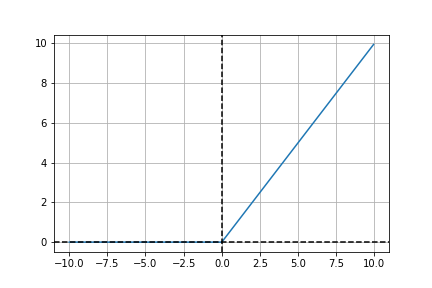
\includegraphics[scale=0.5]{figures/relu.png}
      \caption{Función de activación $ReLU$.}
      \label{fig:nn_relu}
    \end{minipage}
    \hfill
    \begin{minipage}[b]{0.4\textwidth}
      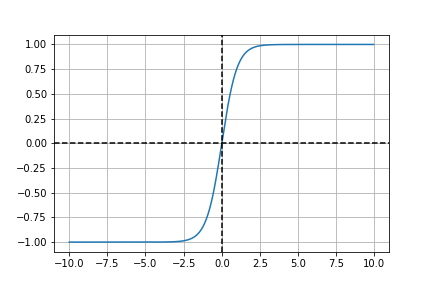
\includegraphics[scale=0.5]{figures/tanh.png}
      \caption{Función de activación $tanh$.}
      \label{fig:nn_tanh}
    \end{minipage}
    \begin{minipage}[b]{0.4\textwidth}
      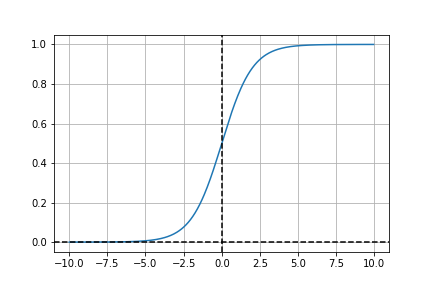
\includegraphics[scale=0.5]{figures/sigmoid.png}
      \caption{Función de activación $\sigma$.}
      \label{fig:nn_sigmoid}
    \end{minipage}
\end{figure}

Notar que la tangente hiperbólica realiza un cambio de escala de la sigmoide
mapeando valores reales al rango $[-1, 1]$ como se muestra en la ecuación \ref{eq:tanh_vs_sigmoid}.

\begin{equation} \label{eq:tanh_vs_sigmoid}
    \tanh\left( x \right) = 2 \sigma(2x) - 1
\end{equation}

En el caso de la \emph{ReLU} cumple el rol de quitar los valores negativos
dejando invariantes los positivos.

\subsection{Variantes de arquitectura y métodos de entrenamiento}

El modelo y procedimiento definido en las secciones \ref{subch:multi_layer_perceptron}, \ref{subch:backpropagation}, conforman una de las
variantes más simples de una red neuronal multicapa. En particular existen
formas de alterar este proceso que aportan permiten dar cierta flexibilidad al
predictor en algunas circunstancias. Una de ellas es la posibilidad de
``apagar`` neuronas aleatoriamente con el fin de evitar el overfitting. Por lo
general a mayor cantidad de capas y neuronas, hay más posibilidad de memorizar los datos de
entrenamiento y obtener no muy buenos resultados en ejemplares nuevos. Es por
eso que este método, denominado \emph{dropout}, puede reducir la complejidad del modelo cada ciertos tramos en el proceso de entrenamiento.

Otra variante es el uso de \emph{batches} al actualizar $\vect{w}$ recopilando el error de varios ejemplares para su posterior propagación a diferencia de procesar a nivel de ejemplos.

También es posible agregar normalización de características en las capas
iniciales de la red neuronal. El uso de escalas distintas en las componentes de
los vectores de entrada puede llevar a ponderar el cálculo del error cometido en una dimensión por sobre otra.

\subsection{XGBoost}

El ultimo modelo de aprendizaje que veremos es \emph{XGBoost} (eXtreme Gradient
Boosting en inglés), un modelo de \emph{ensemble} que consiste en combinar la
respuesta de varios modelos para obtener una final. Es decir, en lugar de
consultar la predicción de un modelo, $K$ de ellos son utilizados. Este tipo de
heurísticas y en particular la de XGBoost han sido enormemente utilizadas por
científico de datos siendo el estado del arte en múltiples problemas de
aprendizaje automático. Desde comparaciones en \emph{benchmarks} hasta
competencias como Netflix prize, Kaggle, y KDDCup.

Otro de los aspectos importantes detrás del éxito de XGBoost es su escalabilidad
en todo tipo de escenarios, siendo muy rápido para manejar consultas de billones
de ejemplos en dominios donde se cuenta con una cantidad limitada de recursos.
Esto motivo aún más su uso en esta tesis, principalmente por la necesidad de
modelos con un rápido tiempo de respuesta durante el proceso de grounding
heurístico.

A diferencia de la regresión logística y las redes neuronales, XGBoost se basa
en una estructura completamente distinta para la definición de sus modelos.
Estas consisten de árboles de decisión donde cada uno aporta su predicción a un
ejemplo de entrada. El objetivo de utilizar varios clasificadores es con la
iniciativa de que se complementen entre sí. Por ejemplo, supongamos que queremos
averiguar si una persona le gusta un videojuego de computadora. Los datos de
entrada serían vectores cuyas componentes representen su edad y la frecuencia en
la que utilizan el ordenador. Si mantenemos dos árboles para cada una de estas
componentes podemos complementar sus respuestas figura (figura \ref{fig:xgboost_tree}) que en lugar de tener solo uno (figura \ref{fig:xgboost_two_tree}).

\begin{figure}
    \centering
    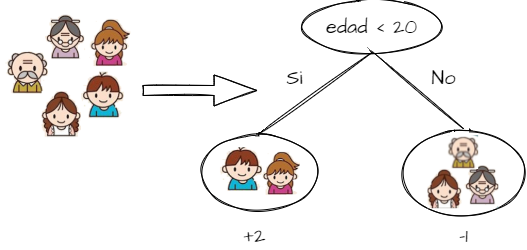
\includegraphics[scale=0.4]{figures/xgboost_tree.png}
    \caption{Árbol que decide por edad de las personas si le interesa un videojuego de computadora. Imagen adaptada de \citep{Tianqi-2016}}
    \label{fig:xgboost_tree}
\end{figure}

\begin{figure}
    \centering
    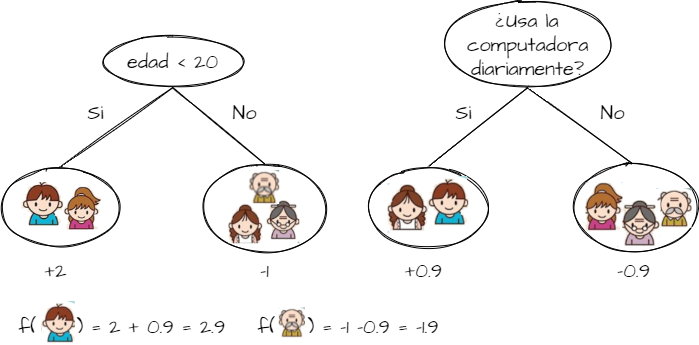
\includegraphics[scale=0.4]{figures/xgboost_two_tree.png}
    \caption{Dos arboles que en base a la edad y uso de la computadora deciden si una persona le interesa un videojuego. Imagen adaptada de \citep{Tianqi-2016}}
    \label{fig:xgboost_two_tree}
\end{figure}

Nuevamente consideremos un conjunto de datos etiquetados $\{(\vect{x}_1, y_1),
..., (\vect{x}_n, y_n)\}$ donde cada $\{\vect{x}_i \in \mathbb{R}^{D}\}$. Un
modelo de \emph{ensemble} del tipo \emph{boosting tree} puede escribirse
matemáticamente como una suma de $K$ funciones que dependan de un ejemplo
$\vect{x}_i$.

\begin{equation} \label{eq:xgb-model-1}
    \hat{y_{i}} = \sum_{k=1}^{K} f_{k} \left( \vect{x}_{i}\right)
\end{equation}

Donde cada $f_k \in \mathcal{F}$, siendo $\mathcal{F}$ la familia o espacio de todos los árboles. Ahora bien, ¿Como están definido cada uno de
los árboles de decisión $f_k$?¿De qué forma son los elementos en $\mathcal{F}$?
¿Cuales son los parámetros del modelo?.

Debemos representar matemáticamente la
estructura del árbol que asigne un ejemplo de entrada $\vect{x}$ a una
correspondiente hoja y por ende a un puntaje como vimos en la figura X. Los
parámetros a encontrar son tales puntajes y se suele referir a ellos como los
pesos del modelo. Otro factor importante es la manera en que se determina la
estructura que debe tener cada árbol.

Formalmente $\mathcal{F} = \{f(\vect{x}) = w_{q\left( \vect{x} \right)}\}$ donde
$q : \mathbb{R}^{D} \rightarrow T$ y $\vect{w} \in \mathbb{R}^{T}$. Aquí $q$
representa el mapeo de un ejemplo $\vect{x}$ una hoja en el árbol. $T$ es el
número de hojas de este último. Y $w_{q\left( \vect{x} \right)}$ es una
componente de $\vect{w}$ que representa el puntaje asociado al ejemplo
$\vect{x}$ según la estructura del árbol determinada por $q$.

Luego como los modelos vistos hasta ahora, para determinar los pesos $\vect{w}$
y la estructura del árbol es necesario definir una función objetivo a minimizar
compuesta por una función de costo y su regularización. No obstante, aprender la
estructura es mucho más complejo que solo utilizar algún método del tipo
descenso por el gradiente. Es por eso que la estrategia utilizada por los
algoritmos de \emph{boosting} es agregar de manera iterativa un nuevo árbol a lo
aprendido, en particular, aquellos árboles que optimicen algún objetivo. Esto da
lugar a definir la predicción del modelo al paso $(t)$.

\begin{align*}
    \hat{y_i}^{(0)} &= 0 \\
    \hat{y_i}^{(1)} &= f_{1}\left( \vect{x}_i \right) = \hat{y_i}^{(0)} + f_1{(\vect{x}_i)} \\
    ... \\
    \hat{y_i}^{(t)} &= \sum_{k=1}^{t} f_{k} \left( \vect{x}_{i}\right) = \hat{y_i}^{(t - 1)} + f_t{(\vect{x}_i)}
\end{align*}

Luego, la función a optimizar en la iteración $(t)$ se define como:

\begin{align}
    \mathcal{L}^{(t)} &= \sum_{i=1}^{n} \ell\left( y_i, \hat{y_i}^{(t)} \right) + \Omega(f_t) \\
                      &= \sum_{i=1}^{n} \ell\left( y_i, \hat{y_i}^{(t - 1)} + f_t{(\vect{x}_i)} \right) + \gamma T + \frac{1}{2} \lambda \sum_{j=1}^{T} w_{j}^{2}
\end{align}

Con $\Omega(f_t)$ la regularización para el predictor. $\gamma$ y $\lambda$ son parámetros de $\Omega$ que intensifican o disminuyen la regularización.

El último requerimiento es optimizar $\mathcal{L}$ para un paso arbitrario y el
significado de la función de costo $\ell$. XGBoost admite cualquier función de
perdida que aproxima a partir de una expansión de Taylor de segundo orden.

\begin{equation} \label{eq:xgboost-loss-taylor}
    \mathcal{L}^{(t)} = \sum_{i = 1}^{n} [
        \ell\left(y_i,
                  \hat{y_{i}}^{(t-1)}
            \right) +
                g_i f_t(\vect{x}_i) +
                \frac{1}{2} h_i f_t^{2}(\vect{x}_i)
        ] + \gamma T + \frac{1}{2} \lambda \sum_{j=1}^{T} w_{j}^{2}
\end{equation}

Donde $g_i$ y $h_i$ son definidas como:

\begin{align}
    g_i &= \partial_{\hat{y_{i}}^{(t-1)}} \ell\left(y_i, \hat{y_{i}}^{(t-1)}\right) \\
    h_i &= \partial_{\hat{y_{i}}^{(t-1)}}^{2} \ell\left(y_i, \hat{y_{i}}^{(t-1)}\right)
\end{align}

Algo a notar de la ecuación \ref{eq:xgboost-loss-taylor} es que $\sum_{i =
1}^{n} \ell\left(y_i, \hat{y_{i}}^{(t-1)} \right)$ es una suma realizada hasta
un paso anterior, estando ya calculado por el algoritmo y por lo tanto se
considera constante para el paso actual $(t)$. Omitiendo dicho término se
obtiene:

\begin{align}
    \mathcal{L}^{(t)} &= \sum_{i = 1}^{n} [
        g_i f_t(\vect{x}_i) +
                \frac{1}{2} h_i f_t^{2}(\vect{x}_i)
        ] + \gamma T + \frac{1}{2} \lambda \sum_{j=1}^{T} w_{j}^{2} \\
                      &= \sum_{i = 1}^{n} [ \label{eq:xgboost-loss-final}
                        g_i w_{q(\vect{x}_i)} +
                                \frac{1}{2} h_i w_{q(\vect{x}_i)}^{2}
                        ] + \gamma T + \frac{1}{2} \lambda \sum_{j=1}^{T} w_{j}^{2}
\end{align}

Se puede identificar la penalización de la función de costo que se agrega al
peso $w_j$ como $G_{j} = \sum_{i \in I_j} g_i$ y $H_j = \sum_{i \in I_j} h_i$
con $I_j = \{i | q(\vect{x}_i) = j\}$ (Conjunto de índices de ejemplares que son
asignados a la $j$-ésima hoja). Es decir, cada componente $w_j$ es penalizada
$|I_{j}|$ veces por $g_i$ y por $h_i$. Luego la ecuación
\ref{eq:xgboost-loss-final} se puede escribir como:

\begin{equation}
    \mathcal{L}^{(t)} = \sum_{j = 1}^{T}[G_j w_j + \frac{1}{2} (H_j + \lambda)w_j^2] + \gamma T
\end{equation}

Finalmente, igualando a $0$ y despejando $w_j$ se obtienen los $w_j$ óptimos para
un árbol con estructura $q(\vect{x})$ y la mejor forma de evaluar su performance
son los de las ecuaciones \ref{eq:xgboost-best-w} y \ref{eq:xgboost-best-opt}.

\begin{align}
    w_{j}^{*} &= - \frac{G_j}{H_j + \lambda} \label{eq:xgboost-best-w}\\
    \mathcal{L}^{*} &= -\frac{1}{2} \sum_{j=1}^{T} \frac{G_{j}^{2}}{H_j + \lambda} + \gamma T \label{eq:xgboost-best-opt}
\end{align}

En resumen, para una estructura de árbol dada, cada ejemplo es evaluado
asignandole una hoja. Se recopilan los ejemplos que pertenecen a cada una de
ellas y se penaliza según los estadisticos $g_i$ y $h_i$ y finalmente obtener el
error cometido por el árbol $\mathcal{L^{*}}$. Aquel árbol que tenga menor error
es el mejor para ser incluido en la iteración actual.

\section{Codificación de características}

Una vez revisado los modelos de aprendizaje, otro factor importante para obtener un buen modelo de machine learning es la representación de los datos de entrada. Preparar los ejemplares para acoplarse apropiadamente a un algoritmo con el fin de mejorar la performance del modelo es una de las tareas las cuales los
científicos de datos disponen la mayor parte de su atención y tiempo. Alguna de
las obligaciones que incluye son la imputación de valores faltantes, manejo de
valores atípicos, estandarización y escalado, transformación de características
numéricas a categóricas, y codificación.

En particular pondremos nuestro foco en la codificación de características
desarrollando métodos del tipo \emph{one-hot} y \emph{word embeddings}.

\subsection{One-hot encoding}
\label{method:ohe}

A menudo los datos disponibles presentan características que no están dadas en
un espacio continuo si no más bien categórico. Por ejemplo, se podría describir
el continente de un país por las clases \emph{inAsia}, \emph{inAfrica},
\emph{inEurope}, \emph{inSouthAmerica}, \emph{inNorthAmerica} siendo
eficientemente representables con enteros $[0, 1, 2, 3, 4]$. De esta manera, si
tenemos un variable que puede tomar una serie de valores categóricos, entonces se puede enumerar cada uno de sus objetos. Esta representación es conocida como \emph{ordinal encoder}.

\begin{equation*}
    \begin{bmatrix}
         & inContinent\\
        Argentina & 3 \\
        Brasil & 3 \\
        España & 2 \\
        USA & 4  \\
        Italia & 2 
    \end{bmatrix}
\end{equation*}

Otra opción es usar un esquema \emph{one-of-K} que
transforma una característica categórica con $N$ clases, en $N$ categorias
binarias con una de ellas 1 y el resto 0. Para el ejemplo anterior tendríamos:

La misma técnica es válida si se quisiera representar oraciones o documentos del
lenguaje natural. Supongamos que tenemos los documentos.

\begin{center}
    $D_1$: ``El sol es una estrella, no es un planeta.`` \\
    $D_2$: ``La tierra es un planeta.``    
\end{center}

Basado en  estos dos textos, un vocabulario de 9 palabras distintas es
construido. Por lo tanto cada documento es representado como un vector de 9
dimensiones.

\begin{equation*}
    \begin{bmatrix}
        & El & sol & es & una & estrella & no & un & planeta & tierra \\
        D_1 & 1 & 1 & 2 & 1 & 1 & 1 & 1 & 1 & 0  \\
        D_2 & 0 & 0 & 1 & 0 & 0 & 0 & 1 & 1 & 1 
    \end{bmatrix}
\end{equation*}

Observar que para este caso una codificación ordinal no sería adecuada dado que
se deberían enumerar todas las palabras del vocabulario.

\subsection{Vectores de palabras (Word embeddings)}
\label{method:wb}

Un vector denso de palabras (comúnmente conocido como word embedding, en inglés)
es una de las técnicas de representación de vocabulario más popular en el área
del procesamiento de lenguaje natural.

Si bien hay distintas formas de representar palabras en una serie de documentos,
los word embeddings proveen otra perspectiva que busca encontrar una
representación vectorial compacta donde cada dimensión logre capturar las
propiedades subyacentes y latentes de la palabra. De esta manera, los embeddings
son superiores a una representación que permanece en un nivel poco profundo.

Su principal característica  es que las expresiones relacionadas entre sı́ (ya
sea por contexto, semántica o sintaxis) se encuentren cercanas en el espacio
vectorial al cual se proyectan. Por ejemplo, si tenemos las oraciones: ``Que
tengas una buena mañana`` y ``Que tengas una buena tarde``. Difieren
semánticamente solo por las palabras ``mañana`` y ``tarde``. No obstante, se
utilizan en contextos similares, lo cual esperaríamos que estén cercanas
vectorialmente.

Otro ejemplo muy famoso que deja en evidencia el concepto de \emph{analogía} en
word embeddings, es el que se muestra en la Figura \ref{fig:king-queen-example}.
En ella se identifican por medio de barras de colores la dimensión de los
vectores asociados a las palabras \emph{king}, \emph{man}, \emph{woman},
\emph{queen}, y la operación vectorial \emph{king - man + woman}. Cada dimensión
se encuentra en la escala de $[-2, 2]$ y se le asigna el color de rojo para
valores cercanos al extremo derecho, azul para las del extremo izquierdo, y
blanco para las que se encuentren alrededor del 0.  Algo a notar es que
\emph{man} y \emph{woman} son mucho más similares de lo que cada uno es con
\emph{king} o \emph{queen}. Otro aspecto interesante son las franjas roja y azúl
que se muestran para cada uno de los ejemplos, indicando que son parecidos en
tal dimensión. Probablemente corresponda a alguna característica humana aunque
se desconoce que puedan llegar a significar debido a la poca interpretabilidad
del espacio al cual se proyectan.

Aun así, lo importante es la comparación entre palabras. Dado que ahora tienen
una representación vectorial, se pueden sumar o restar obteniendo nuevos
resultados que forman parte del espacio. Este es el caso del vector dado por
\emph{king - man + woman}. No conocemos que dimensiones exactamente capturan que
rey es utilizado para identificar al monarca de un reino, pero se puede
substraer el caracter masculino del vector \emph{man} y agregar las de
\emph{woman} esperando que se aproximen a las de \emph{queen}.
Sorprendentemente, de un total de 400000 palabras sobre las cuales se realizó el
experimento, reina fue la palabra más cercana. Los detalles del mismo se pueden
ver desde \footnote{\url{https://jalammar.github.io/illustrated-word2vec/}}.

\begin{figure}
    \centering
    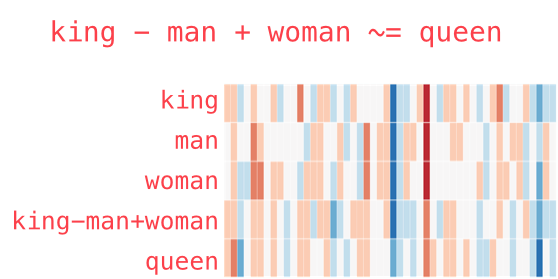
\includegraphics[scale=0.68]{figures/king-analogy-viz.png}
    \caption{Vectores de palabras para ``king``, ``man``, y ``woman``}
    \label{fig:king-queen-example}
\end{figure}

Esto refleja el gran potencial que tienen los word embeddings y su importancia
para estudiarlos como métodos de codificación. A continuación analizaremos como
se calculan dichas representaciones y que algoritmos fueron finalmente
utilizados en esta tesis.

\subsubsection{Modelos de lenguaje}

Después de ver el potencial de los embeddings, surge la pregunta, ¿Cómo
funcionan internamente? ¿De qué manera se obtienen estos vectores de palabras?
En \citep{firth-57} se mostró que el significado de una palabra está determinado
según sus palabras vecinas. Si contemplamos la oración ``Que tengas un buen`` y
se quisiese averiguar cual es la expresión que le sigue, lo más probable es que
las palabras días, tarde, noche, o semana, hayan sido las primeras candidatas.
Este tipo de tareas en las que se intenta predecir información de la oración a
partir del contexto o viceversa son denominadas tareas de pretexto y son
utilizadas para entrenar un clasificador que resuelva esta tarea, únicamente
para preservar su representación a nivel de palabras.

\subsubsection{Skipgram}

Es un método desarrollado en \citep{Mikolov-2013} cuyo objetivo es, para un
vocabulario de tamaño $W$ donde una palabra es identificada por su índice $w \in
\{1, ... W\}$, aprender una representación vectorial para cada $w$. Estas
representaciones son entrenadas para predecir palabras vecinas a partir de una
actual. Es decir, dado un largo corpus de entrenamiento, considerarlo como una
sola secuencia de palabras $w_1, ... w_T$ y maximizar la expresión en \ref{eq:skipgram-ideal}

\begin{equation} \label{eq:skipgram-ideal}
    \frac{1}{T} \sum_{n=1}^{T}
                    \sum_{c \in C_t} \log P(w_c | w_t)
\end{equation}

Donde $C_t$ es el conjunto de indices de palabras que rodean a $w_t$. La
probabilidad de observar una palabra del contexto $w_c$ dado $w_t$ es modelada a
partir de sus vectores representación. Por el momento, abstraeremos esto a
partir de una función \emph{score} $s$ que mapea pares (palabra, contexto) a un
puntaje en $\mathcal{R}$. Una forma posible de definir la probabilidad de una palabra en
el contexto es por medio de la función \emph{softmax}.

\begin{equation} \label{eq:skipram-softmax}
    P(w_{c}|w_{t}) = \frac{e^{s(w_t, w_c)}}{\sum_{j=1}^{W} e^{s(w_t, j)}}
\end{equation}

No obstante, este calculo es bastante costoso computacionalmente siendo que al
final solo es de interés predecir una palabra del contexto $w_c$ dado una
palabra $w_t$. Es por eso que el problema puede ser visto como una tarea de
clasificación binaria en lugar de una multiclase. El objetivo es predecir
independientemente la presencia o ausencia de palabras de contexto. Para una
palabra en la posición $t$, consideramos todos los contextos como ejemplos
positivos, y palabras seleccionadas aleatoriamente del vocabulario, como
negativos. Para un contexto $c$, utilizando la función de costo \emph{binary
logistic}, obteniendo la siguiente función de probabilidad:

\begin{equation}
    \log\left( 1 + e^{-s(w_t, w_c)} \right) +
    \sum_{n \in \mathcal{N}_{t, c}} \log\left( 1 + e^{s(w_t, n)} \right)
\end{equation}

Donde $\mathcal{N}_{t, c}$ es una muestra aleatoria de ejemplares negativos
tomadas del vocabulario. Si denotamos la función logística como $\ell: x \mapsto
\log \left(1 + e^{-x} \right)$, podemos reescribir la función a optimizar del
problema como:

\begin{equation}
    \sum_{n=1}^{T} 
        \sum_{c \in C_t} \ell\left(s(w_t, w_c)\right) +
        \sum_{n \in \mathcal{N}_{t, c}} \ell\left(-s(w_t, n) \right)
\end{equation}

Una parametrización natural para $s$ entre una palabra $w_t$ y un contexto $w_c$
es a partir del uso de vectores de palabras. Definimos dos vectores $\vect{u}_w$
y $\vect{v}_w$ en $\mathbb{R}^D$ también conocidos como vectores \emph{input} y
\emph{output}. Es decir, tenemos vectores $\vect{u}_{w_t}$ y $\vect{v}_{w_c}$
asociados a palabras $w_t$ y $w_c$. Luego el \emph{score} puede computarse como
$s\left( w_t, w_c \right) = \vect{u}_{w_t}^\top \vect{v}_{w_c}$.

Para ejemplificar como es el proceso de entrenamiento de este modelo, tomemos la
secuencia ``Me gustaría dos rebanadas de pizza mozzarella``. Podemos pensar un
contexto como una ventana que se desliza a través del conjunto de entrenamiento.
La figura \ref{fig:wb_slices} muestra las 3 posibles ventanas de tamaño 5 que se pueden obtener
a partir de la secuencia deslizándose con un paso de 1.

Con cada ventana, seleccionamos aquella palabra que cargue más valor
informativo, que por lo general suele ser la del medio, y la utilizamos para
predecir sus vecinas. De esta manera, generamos un conjunto de entrenamiento
compuesto por pares (palabra, palabra de contexto) donde etiquetamos con 1, si
ambas son vecinas, y 0 en caso contrario. El resultado final para cada contexto
se puede ver en la figura \ref{fig:wb_all_ones_matrix}. Esta es la simplificación del problema para
trabajar sobre una tarea de clasificación binaria. En lugar de ser multiclase
cuya  etiqueta sería la palabra de contexto, la incluimos como característica y
reemplazamos las anotaciones por 1's y 0's. Ahora bien, con nuestros datos
actuales solo tendríamos etiquetas con 1's. En tal caso, el modelo en lugar de
aprender lo que necesitamos, estaría sesgado a siempre predecir afirmativamente.
Es por eso que agregar ejemplos negativos de manera aleatoria (figura \ref{fig:wb_neg_sampling_matrix}) a
cada $w_t$ resulta una buena idea.

\begin{figure}
    \centering
    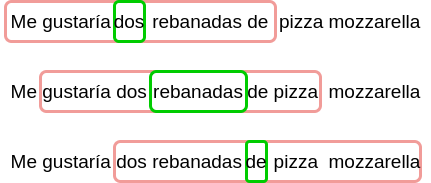
\includegraphics[scale=0.60]{figures/context_example_1.png}
    \caption{Todas las ventanas de contexto con tamaño 5 que se pueden formar con la frase
             ``Me gustaría dos rebanadas de pizza mozzarella``.}
    \label{fig:wb_slices}
\end{figure}

\begin{figure}
    \centering
    \begin{minipage}[b]{0.4\textwidth}
      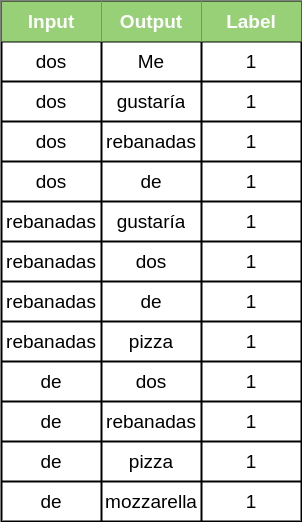
\includegraphics[scale=0.5]{figures/context_example_2.png}
      \caption{Material de entrenamiento obtenido de las ventanas.}
      \label{fig:wb_all_ones_matrix}
    \end{minipage}
    \hfill
    \begin{minipage}[b]{0.4\textwidth}
      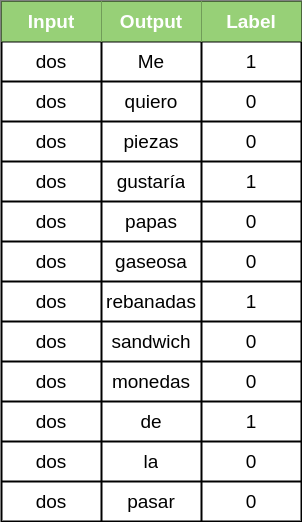
\includegraphics[scale=0.5]{figures/context_example_3.png}
      \caption{Selección aleatoria de 2 ejemplos negativos por cada positivo.}
      \label{fig:wb_neg_sampling_matrix}
    \end{minipage}
\end{figure}

Luego, al inicio del proceso de entrenamiento se crean dos matrices con valores
aleatorios, una para los embeddings y otra para los contextos. Estas dos
matrices de tamaño $V \times D$, tienen una fila por cada palabra en el
vocabulario. En este caso, $D$ es la cantidad de dimensiones que tendrán sus
representaciones. En cada paso de entrenamiento, se selecciona un ejemplo
positivo y sus correspondientes ejemplos negativos (figura \ref{fig:wb_emb_con_matrix}). Este grupo es
evaluado por el modelo a partir de los vectores representación \emph{input} y
\emph{output} según el producto escalar entre ellas y su conversión en
probabilidades por medio de la función sigmoide. A partir de la etiqueta
real, se puede determinar el puntaje de error para cada ejemplo y finalmente
actualizar los parámetros de las matrices de embeddings y contexto. Eso concluye
un paso de entrenamiento, que se repite por cada grupo de ejemplos positivos y
negativos por una cierta cantidad de épocas. Una vez concluido el proceso de
entrenamiento, la matriz de embeddings contiene las representaciones finales.

\begin{figure}
    \centering
    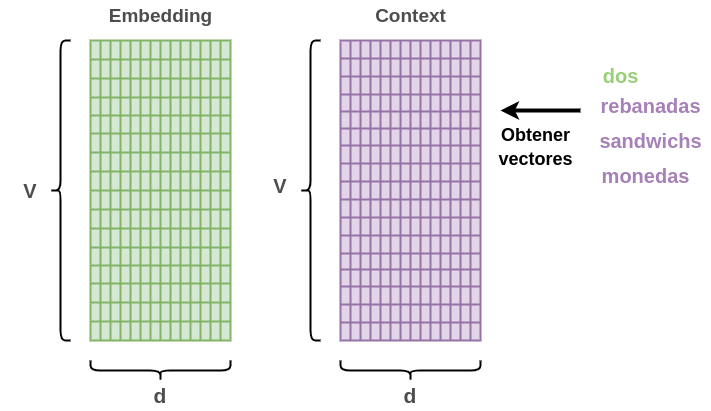
\includegraphics[scale=0.5]{figures/context_example_4.png}
    \caption{Matrices para los embeddings y contextos.}
    \label{fig:wb_emb_con_matrix}
\end{figure}

\subsubsection{Modelos de lenguaje a nivel de subpalabra}
\label{method:wb_subwords}

El modelo de skipgrams al usar vectores representación por cada palabra se
ignora su estructura interna. Esto fue lo que inspiró el estudio de modelos a
nivel de subpalabra en \citep{bojanowski-2017}. La principal característica de estos modelos
radica en la función de score $s$. En lugar de considerar una palabra $w$ en su
totalidad, esta es dividida en $n$-gramas de caracteres. Para delimitar inicio y
fin de una palabra se agregan símbolos especiales \verb|<| y \verb|>| respectivamente. Esto a
su vez permite distinguir prefijos y sufijos de otras secuencias de caracteres.
Por último la palabra $w$ también es incluida como un $n$-grama o secuencia
especial. Por ejemplo, la palabra \emph{color} y $n=4$ estaría representada por
los $4$-gramas:

\begin{center}
    \verb|<col|, \verb|colo|, \verb|olor|, \verb|lor>|
\end{center}

Junto a la secuencia completa \verb|<color>|. Notar que la secuencia
\verb|<olor>| correspondiente a la palabra \emph{olor} es diferente al $4$-grama
\verb|olor|. Luego lo único que queda restante es modificar la función
\emph{score} $s$ del método skipgram por la ecuación \ref{eq:wb_subwords_s_score}.

\begin{equation} \label{eq:wb_subwords_s_score}
    s\left(w, c\right) = \sum_{g \in \mathcal{G}_w} \vect{z}_g^{\top}\vect{v}_c
\end{equation}

Donde, $\mathcal{G}_w \subset \{1, .. G\}$ es el conjunto de $n$-gramas de la palabra $w$, $\vect{z}_g$ el vector representación del $n$-grama $g$, y $G$ la cantidad de $n$-gramas en total.

Este modelo permite compartir representaciones entre palabras logrando aprender
una confiable codificación a palabras poco comunes siendo útil para los
experimentos de esta tesis en la tarea de codificación de planes relajados.

\subsubsection{Representación vectorial de oraciones}
\label{lit:sentence_vector}

Como cierre de esta sección presentaremos algunos métodos sencillos de codificación de oraciones a partir de los embeddings orientadas a tareas de clasificación que involucren manipulación de texto.

\textbf{Concatenación}. Este método consiste en concatenar los vectores de las
palabras que conforman la oración a codificar obteniendo un vector de largo
igual a la suma de las dimensiones de los vectores individuales. En este caso,
el problema evidente que surge es la representación de oraciones con distinto
largo y el tamaño del vector resultante.

\textbf{Promedio}. Como su nombre lo indica, este método computa el centroide de
los embeddings de todas las palabras que conforman una oración. Usualmente esta
codificación resulta ser adecuada siempre y cuando los vectores de las palabras
se encuentren en la misma escala, lo cual no siempre suele ser el caso. Otro
problema menos evidente es la posibilidad de ocurrencia de palabras poco
representativas pero que tengan mucho peso en la suma debido a la frecuencia en que ocurren. Si en la oración la palabra que buscamos ocurre pocas veces puede verse opacada.

\textbf{Promedio normalizado}. Por último, una mejora de la representación
anterior es la normalización por norma L2 de cada vector previo a realizar el
promedio.

Pueden encontrarse otras maneras de codificar los datos a través de \citep{Iacobacci-2016}
donde se explican como utilizar word embeddings para desambiguación de sentidos,
proponiendo distintos métodos de codificación de instancias de entrenamiento a partir
de un modelo de lenguaje. Esto muestra que el uso de representaciones a nivel de palabra en la codificación de oraciones suelen ser patrones comunes al momento de incluirlo en una arquitectura supervisada.

\section{Métricas de clasificación}
\label{lit:metrics}

Con el fin de evaluar que tan bien se desempeña el modelo se contrastan
resultados predichos por el clasificador contra otros previamente anotados que
no formaron parte como material de entrenamiento. Para un problema de
clasificación binaria donde los positivos corresponden con la clase $1$, y los
negativos con la $0$ dispusimos de las siguientes métricas.

\textbf{Precisión}. Cociente entre verdaderos positivos y el total de
predicciones positivas. 

\begin{equation}
    precision = \frac{TP}{TP + FP}
\end{equation}

\textbf{Recall}. Cociente entre verdaderos positivos y el total de positivos.

\begin{equation}
    recall = \frac{TP}{TP + FN}
\end{equation}

\textbf{F-score} ($F_{\beta}$). El inconveniente de las primeras dos métricas es
que ambas alcanzan el $100\%$ en modelos triviales. Es decir aquellos que predicen
siempre la clase positiva obtienen un valor máximo en recall, mientras los que
predicen siempre la clase negativa consiguen un valor máximo en precisión. La
$F_{\beta}$ mide el desbalance entre las dos anteriores ponderando una por sobre
la otra de acuerdo al valor de $\beta$ pero esta vez penalizando los modelos
triviales. 

\begin{equation}
    F_{\beta} = (1 + \beta^2) \frac{precision . recall}{\beta^2 precision + recall}
\end{equation}

Valores comunes de $\beta$ suelen ser $0.5$ (priorizar precisión), $1$ (ninguna
prioridad), $1.5$ (priorizar recall).

\textbf{H-score} ($H_{\beta}$). Durante el desarrollo de la tesis se definió una
variante de la $F_{\beta}$, que denominamos $H_{\beta}$, permitiendo lidiar con
datos desbalanceados. Si la cantidad de datos negativos es mucho mayor que la de
positivos, la precisión puede verse más comprometida que la recall, al haber más
oportunidades de cometer un falso positivo. Para solucionar eso, en vez de
considerar precisión y recall en la ecuación de $F_{\beta}$, se utilizó la
\emph{taza de verdaderos positivos y negativos} (TPR, y TNR).

\begin{align}
    TPR &= \frac{TP}{TP + FN} \\
    TNR &= \frac{TN}{TN + FP} \\
    H_{\beta} &= (1 + \beta^2) \frac{TNR . TPR}{\beta^2 TNR + TPR}
\end{align}

Notar que $TNR$ continua penalizando por la cantidad de falsos positivos de manera
similar a precisión. No obstante, la métrica es relativa a la cantidad de
negativos. Si el desbalance es sobre los negativos, entonces la métrica no se ve
comprometida. De manera similar a $F_{\beta}$, un valor de $0.5$ prioriza $TNR$, de
1 considera un balance entre ambas métricas, y $1.5$ prioriza $TPR$.

\textbf{Gráficos de distribución de predicciones.} Por úĺtimo, la métrica
estrella de este trabajo son los gráfico de distribución de predicciones. Dado
que para el algoritmo de grounding heurístico se utilizan las probabilidades
asignadas a un plan relajado y una acción, un histograma que refleje la
distribución de las probabilidades asociadas a cada par es excelente para
determinar si las clases positivas se distribuyen con una probabilidad mayor que
las negativas.
    
    \part{Metodología}
    \chapter{Etapas de preparación y ejecución de modelos}
\label{ch:method}

Inferir si una hipótesis brindará resultados positivos o negativos en un
proyecto de investigación es una de las tareas más complicadas de conocer con
antelación. Aún investigadores experimentados prueban decenas de ideas antes de
obtener algún descubrimiento concreto. Construir sistemas de aprendizaje
automático usualmente requieren de:

\begin{enumerate}
    \item Una hipótesis inicial la cual construir el sistema.
    \item Una implementación en algún lenguaje de programación.
    \item Ejecución de experimentos que permitan concluir si la idea original
    funciona de acuerdo a lo esperado.
\end{enumerate}

Basado en lo aprendido en esos 3 pasos, se vuelven a plantear nuevas ideas e
iterar sobre este proceso. Mientras más rápido se pueda finalizar un ciclo,
mayor será el progreso en la investigación. Debido a la larga lista de posibles
hipótesis para verificar, se deben obtener resultados prontamente, por lo
general, en a lo sumo una semana de haber iniciado el ciclo. Es por eso que una
prueba de concepto a partir de una implementación prototipo es más importante
que construir un sistema complejo en una etapa temprana de investigación.

No obstante, una vez validadas varias de las hipótesis, empezar nuevas
implementaciones a partir de los prototipos puede llegar a ralentizar el proceso
de desarrollo, ya que ciertos estándares de código no son tenidos en cuenta.
Tales como manejo de excepciones, documentación adecuada, o herramientas de
monitoreo y mantenimiento de código. El objetivo de estas pruebas de concepto es
la de otorgar experiencia a los investigadores para identificar los
requerimientos y resultados iniciales. Esto para luego construir un entorno de
desarrollo en esa dirección.

Durante las pruebas de concepto realizadas durante esta tesis se analizó la
factibilidad de la premisa inicial, encontrar un modelo de aprendizaje
automático a partir de una codificación de datos de planes relajados y acciones
etiquetadas que permitan guiar el proceso de grounding. Sin embargo, a medida
que el proyecto fue necesitando de experimentos más complejos, se agregaron
funcionalidades hasta construir un sistema de experimentación completo,
configurable, adecuado a nuestras necesidades, y que permita otorgar resultados
en el corto plazo de iniciado el ciclo de experimentación. Es por eso que en
este capítulo se describirán los detalles de implementación de cada uno de los
módulos que integran el flujo de ejecución de un experimento, abarcando el
dominio de planning utilizado, especificaciones de tareas STRIPS que se pueden
obtener a partir del dominio, persistencia de datos, preprocesamiento,
entrenamiento, evaluación de modelos, y registro y visualización de resultados.
Esto con el fin de describir los experimentos con mucha más claridad en el
capítulo \ref{ch:results}.
\section{Dominio de planning: Satellite}

\subsection{Descripción del dominio}

Para la construcción del conjunto de datos nos centramos en el dominio de
planning \emph{Satellite}, siendo parte del learninig track de la competencia
internacional de planning (IPC) del año 2011. Este dominio es un modelo del
problema de programación de observación satelital. Este implica el uso de uno o
más satélites para hacer observaciones, recopilar datos, y descenderlos a una
estación terrestre. Los satélites están equipados con diferentes instrumentos,
cada uno con características en términos de objetivos de calibración, producción
de datos, consumo de energía, y requisitos para el calentamiento y enfriamiento.
Los satélites pueden apuntar a diferentes objetivos con el fin de obtener
información de tal objeto. Existen restricciones sobre qué objetivos son
accesibles para un satélite debido a las capacidades de oclusión y rotación. Los
datos que generan los instrumentos de un satélite deben ser enviados a tierra
una vez ocurra una ventana de comunicación terrestre. La meta consiste en hallar
la cobertura (más eficiente) de las observaciones dadas las capacidades de los
satélites.

El cuadro \ref{tb:satellite_stats} resume los esquemas de acción del dominio con
su correspondiente tamaño de interfaz (Int), cantidad de precondiciones atómicas
(Pre), y cantidad de efectos atómicos (Eff). El Listing
\ref{lst:satellite-domain} muestra la especificación del dominio en PDDL.

\begin{table}[h!]
    \centering
    \scalebox{1}{
    \begin{tabular}{||c| c | c | c||} 
    \hline
    Esquema & Int & Pre & Eff\\ [0.5ex] \hline\hline
    %(take_image satellite0 planet5 instrument1 image1)
    take\_image & 4 & 6 & 1 \\ 
    calibrate & 3 & 4 & 1 \\ 
    turn\_to & 3 & 2 & 2 \\ 
    switch\_on & 2 & 2 & 3 \\ 
    switch\_off & 2 & 2 & 2 \\ [1ex] 
    \hline
    \end{tabular}}
    \caption{Ejemplos etiquetados a partir de un plan relajado y una acción}
    \label{tb:satellite_stats}
\end{table}

\begin{lstlisting}[
    float=!htb,
    caption={Dominio Satellite en PDDL.},
    label={lst:satellite-domain},
    language=PDDL]

    (define (domain satellite)
    (:requirements :strips :equality :typing)
    (:types satellite direction instrument mode)
    (:predicates 
             (on_board ?i - instrument ?s - satellite)
             (supports ?i - instrument ?m - mode)
             (pointing ?s - satellite ?d - direction)
             (power_avail ?s - satellite)
             (power_on ?i - instrument)
             (calibrated ?i - instrument)
             (have_image ?d - direction ?m - mode)
             (calibration_target ?i - instrument ?d - direction))
  
    (:action turn_to
     :parameters (?s - satellite ?d_new - direction ?d_prev - direction)
     :precondition (and (pointing ?s ?d_prev)
                        (not (= ?d_new ?d_prev)))
     :effect (and  (pointing ?s ?d_new)
                   (not (pointing ?s ?d_prev))))
   
    (:action switch_on
     :parameters (?i - instrument ?s - satellite)
     :precondition (and (on_board ?i ?s) 
                        (power_avail ?s))
     :effect (and (power_on ?i)
                  (not (calibrated ?i))
                  (not (power_avail ?s))))
   
    (:action switch_off
     :parameters (?i - instrument ?s - satellite)
     :precondition (and (on_board ?i ?s)
                        (power_on ?i))
     :effect (and (not (power_on ?i))
                  (power_avail ?s)))
  
    (:action calibrate
     :parameters (?s - satellite ?i - instrument ?d - direction)
     :precondition (and (on_board ?i ?s)
                        (calibration_target ?i ?d)
                        (pointing ?s ?d)
                        (power_on ?i))
     :effect (calibrated ?i))

    (:action take_image
     :parameters (?s - satellite ?d - direction ?i - instrument ?m - mode)
     :precondition (and (calibrated ?i)
                        (on_board ?i ?s)
                        (supports ?i ?m)
                        (power_on ?i)
                        (pointing ?s ?d)
                        (power_on ?i))
     :effect (have_image ?d ?m))
    )
\end{lstlisting}

\section{Manejo de datos}

\subsection{Generación de tareas de planning}
\label{method:data_generation}

Las instancias de problemas a partir del dominio Satellite se obtuvieron
automáticamente mediante un generador de problemas configurable de acuerdo a las
características que deseamos que tenga. Estas son la cantidad de satélites, la
cantidad máxima de instrumentos, el número de modos, el número de objetivos, y
el número de observaciones. A mayor sea algunos de estos parámetros, mayor el
número de acciones y facts necesarios para resolverlos. Una vez definida una
parametrización que represente las características de la tarea a modelar, el
generador devuelve su representación STRIPS especificada en PDDL.

% \url{https://github.com/AI-Planning/pddl-generators/tree/master/satellite}

Sean $\Pi^{PDDL} = (\mathcal{P}, \mathcal{A}, \Sigma^{C}, \Sigma^{O}, I, G)$ la
representación STRIPS en PDDL dada por el generador de problemas, y $\Pi = (F,
A, I, G)$ su tarea STRIPS asociada. La información que necesitamos recolectar
es:

\begin{enumerate}
    \item Un plan relajado $\vec{a}^{+}$ para $\Pi^{+}$.
    \item Un plan (en lo posible el óptimo) $\vec{a}$ para $\Pi$.
    \item El conjunto de objetos $\Sigma^{O}$.
    \item El conjunto de acciones instanciadas $A$ de $\Pi$.
\end{enumerate}

Los puntos 3, y 5 pueden obtenerse a partir de los archivos PDDL devueltos por
el generador. En cambio, 1, 2, y 4 requieren resolver la tarea por medio del
planificador de Fast Downward para ser obtenidos. Dado que $\Pi$ se obtiene a
partir de Fast Downward, el conjunto $A$ de acciones instanciadas contiene
únicamente aquellas que son alcanzables relajadamente desde el estado inicial
$I$. A su vez, en la medida de lo posible, se intentará obtener el plan óptimo
que resuelve $\Pi$. Esto se debe a la noción de relevancia de una acción para
resolver una tarea STRIPS. En un plan óptimo, las acciones que lo componen son
todas necesarias en la secuencia. Si una acción es eliminada, la secuencia
resultante no puede ser un plan de la tarea debido a que se obtendría un plan
con menos acciones que el plan óptimo y, por lo tanto, una contradicción (Lo cual
no es el caso para un plan genérico).

La información asociada a un problema obtenida por el generador y el
planificador se almacenan en directorios que contienen los siguientes archivos:

\begin{itemize}
    \item \emph{all\_operators.bz2}: Archivo comprimido del conjunto de acciones
    instanciadas.
    \item \emph{objects}: Conjunto de objetos del problema.
    \item \emph{problem.pddl}: Especificación en PDDL del problema.
    \item \emph{relaxed\_plan}: Plan relajado que resuelve la tarea relajada.
    \item \emph{optimal\_plan} o \emph{sas\_plan}: Plan (óptimo) que resuelve la
    tarea.
\end{itemize}

Por último, queda mencionar que tipo de problemas se generaron. Se dividieron en
3 grupos principales de acuerdo a su dificultad. 240 problemas a los cuales
pueden resolverse de manera óptima por el planificador, 48 a los cuales solo un
plan fue encontrado, y 18 que no pudieron resolverse debido a una falla en el
proceso de grounding. Es sobre este último grupo que nos interesa realizar
inferencia sobre las acciones que puedan ser relevantes para resolverlo y en los
que el modelo de aprendizaje automático debe guiar durante el proceso de
grounding. Es por eso que estos 25 problemas fueron elegidos para formar parte
de los problemas de test. Mientras que aquellos que sí logran resolverse (de
manera óptima o no) forman parte del material de entrenamiento.

Como veremos en la sección \ref{method:labeling}, requeriremos de los planes
reales para etiquetar estos datos y poder de esta forma realizar un análisis del
comportamiento del modelo. Por lo que es necesario encontrarles una solución a
los problemas de test. Afortunadamente, Satellite es uno de los dominios
trabajados en \citep{Gnad_Torralba_Dominguez_Areces_Bustos_2019} por lo que
limitaremos los problemas de test a aquellos problemas para los que una
solución fue hallada en este trabajo.

Otro inconveniente en los problemas de test, es la ausencia de las acciones
instanciadas para resolverlo. Aún habiendo logrado calcular un plan de la tarea,
la cantidad de instancias alcanzables relajadamente en $A$ es muy grande por la
cual no son dadas por el planificador al terminar el proceso de grounding, como
sí es el caso de los datos entrenamiento. Para resolver este problema, solo se generó
una muestra aleatoria de acciones instanciadas obtenidas a partir de grounding
cartesiano, por fuera del planificador.

Por lo tanto, tomaremos provecho de estas soluciones como una manera de
verificar que el modelo de aprendizaje logra desempeñarse correctamente antes de
probarlo en el planificador en tareas que no puedan instanciarse.

\subsection{Preservación de datos}

Una vez identificado qué problemas son utilizados como entrenamiento y cuáles como
test, es necesario preservar estos datos de manera organizada y de fácil acceso.
Si bien los datos se encuentran en archivos en una cierta estructura, no pueden
ser extraídos de manera programática. Por tal razón se tabularon y almacenaron
los datos en una base de datos relacional, para su posterior acceso por medio de
una herramienta de consultas.

Para el almacenamiento utilizamos una base de datos relacional de tipo SQL. La
figura \ref{fig:ERD} muestra su diagrama de entidad relación.

\begin{figure}[t!]
    \centering
    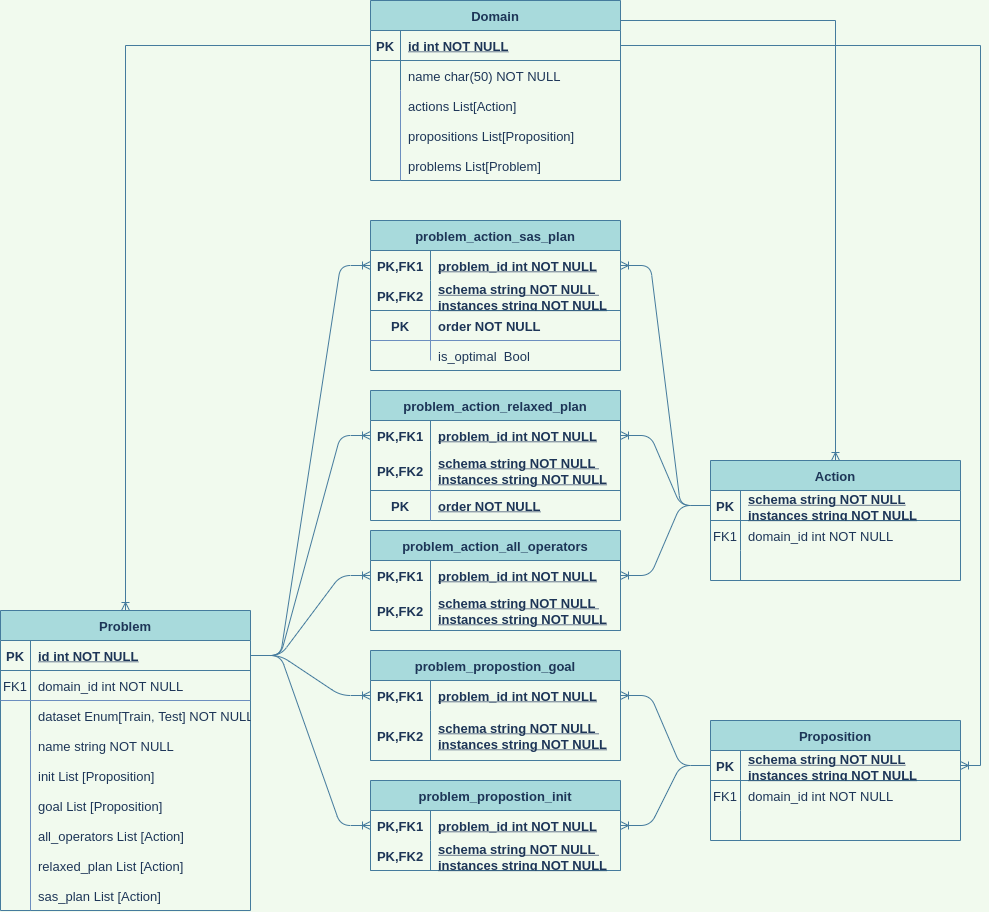
\includegraphics[width=\linewidth]{figures/ERD.png}
    \caption{Diagrama de entidad relación de la base de datos.}
    \label{fig:ERD}
\end{figure}

La tabla \emph{Problem} representa el conjunto de problemas. Algunas de sus
propiedades son, el nombre del problema (nombre dado por el generador), y el
conjunto al cual pertenece (entrenamiento o test). Para representar en la base
de datos tanto los planes relajados, como los planes que resuelven la tarea, se
utilizan relaciones \emph{many-to-many} a la tabla de acciones, manteniendo una
tabla intermedia que relaciona un problema con las acciones que conforman el
plan. Dado que las tablas en bases de datos relacionales se definen a partir de
la teoría de conjuntos, la repetición y el orden puede perderse para las
acciones que ocurren en un plan. Para resolver este problema se agregó el orden
de manera explícita como atributos en sus tablas. Ahora bien, notar que la tabla
\emph{Problem} tiene como atributos 2 listas, donde cada atributo representa de
manera ordenada (según algún criterio, en nuestro caso, el de los planes
relajados) los planes relajados, y los planes reales. Esto permite accederlos de
una manera mucho más práctica sin tener que utilizar el atributo del orden de
manera explícita al realizar una consulta. Para almacenar el conjunto de
acciones instanciables, el estado inicial, y la meta de un problema, simplemente
se utilaron otras tablas intermedias pero sin la necesidad de mantener el orden
esta vez.

Las tablas \emph{Action} y \emph{Proposition} almacenan todas las acciones y
facts instanciables relajadamente que hayan ocurrido en cualquier problema. Para
evitar repeticiones se agregó como clave primaria el nombre del esquema junto
con el de sus parámetros.

Por último, la tabla \emph{Domain} mantiene registro del dominio en caso de que
busquemos utilizar múltiples dominios además de Satellite en nuestros
experimentos.

Para realizar consultas a la base de datos empleamos un \emph{object relational
mapping} (ORM) que permite gestionar el acceso por medio de un lenguaje de
programación. El ORM considera cada tabla como una clase y elementos de la tabla
como objetos de tal clase. Por lo tanto, al efectuar una consulta el ORM mapea
los elementos partícipes de esa consulta a objetos del lenguaje de programación
Eso incluye cualquier otra relación u objeto que esté involucrado en la consulta
de manera directa o indirecta, cono es el caso del plan relajado, o el plan que
resuelve la tarea. De esta manera el ORM dispone al programador de todo el poder
de la programación orientada a objetos para manipular los datos.

\subsection{Etiquetado de ejemplos}
\label{method:labeling}

A partir de la base de datos es necesario generar una \emph{matriz de
entrenamiento} que será dada como entrada al modelo de aprendizaje automático.
En particular, mencionamos qué problemas se van a usar para entrenar los modelos
y cuáles para evaluarlos. Pero aún nos queda explicar cuál es la estructura
explicita de los pares $\{(\vect{x}_1, y_1), ..., (\vect{x}_n, y_n)\}$ de los
conjuntos de entrenamiento y test que recibirán como entrada los modelos
mencionados en el capítulo \ref{ch:lit_ml}.

Dado que buscamos aprender un modelo que prediga si una acción es relevante para
el plan real de un problema, necesitamos incluir en $\vect{x}$ información de
tal problema y la acción a cuál queramos averiguar su relevancia. Además, debe
ser fácil de calcular, tanto para las tareas de entrenamiento como las de test.
Como mencionamos en la sección \ref{lit:delete_relaxed}, para una tarea
especificada en PDDL, el planificador instancia el problema y realiza una
búsqueda exhaustiva guiada por medio de una función heurística definida usando
planes relajados. Si los planes relajados permiten guiar la búsqueda para
encontrar un plan de la tarea, entonces también podrían ser usados para guiar el
proceso de grounding. Por lo tanto, la estructura de los vectores de entrada
incluirán tanto el plan relajado como la acción que queremos estimar.

Por otro lado, en la sección \ref{method:data_generation} no sólo obtuvimos el
plan relajado de cada tarea generada, sino además el plan que lo resuelve junto
a las instancias de las acciones alcanzables relajadamente durante el proceso de
grounding. Por lo tanto, para una tarea en particular (y por ende un plan
relajado), se pueden identificar dos clases distintas de acciones generadas:

\begin{enumerate}
    \item Las acciones que pertenecen a la solución (óptima o no).
    \item Las acciones que no pertenece a la solución, pero que sí fueron
    generadas por el proceso de grounding por alcanzabilidad relajada de Fast
    Downward.
\end{enumerate}

A las acciones de 1 las denominamos \emph{good operators} de la tarea, y las de
2, \emph{bad operators} de la tarea. A estos dos conjuntos los denotaremos con
$A^{good}$ y $A^{bad}$ respectivamente.

\begin{algorithm}
    \caption{}\label{alg:training_data}
    \begin{algorithmic}
    \Require Plan relajado $\vec{a}^{+}$, $A^{good}$, y $A^{bad}$ de una tarea
    de la sección \ref{method:data_generation} \Ensure Matriz de ejemplos $M$ de
    tamaño $(|A^{good}| + |A^{bad}|) \times 3$ \State $M \gets [\ ]$ \For{$a \in
    A^{good} $} \State $M.push\_back((\vec{a}^{+}, a, 1))$ \EndFor
    
    \For{$a \in A^{bad} $} \State $M.push\_back((\vec{a}^{+}, a, 0))$ \EndFor
    
    \State \Return $M.to\_array()$
    \end{algorithmic}
\end{algorithm}

El algoritmo \ref{alg:training_data}, dado el plan relajado de un problema
y los conjuntos $A^{good}$ y $A^{bad}$, genera los datos etiquetados de una sola
tarea obteniendo una matriz como se muestra en el cuadro \ref{tb:matrix_shape}.

\begin{table}[h!]
\centering
\scalebox{0.9}{
 \begin{tabular}{||c | c | c||} 
 \hline
 Plan relajado & Acción & Etiqueta \\ [0.5ex] \hline\hline
 %(take_image satellite0 planet5 instrument1 image1)
 {}[switch\_on instrument0 satellite0, take\_image ...] & calibrate satellite0
 instrument0 star4 & 1 \\
 {}[switch\_on instrument0 satellite0, take\_image ...] & switch\_on instrument0
 satellite0 & 1 \\
 {}[switch\_on instrument0 satellite0, take\_image ...] & switch\_on instrument3
 satellite1 & 1  \\
 ... & ... & ...  \\
 {}[switch\_on instrument0 satellite0, take\_image ...] & turn\_to satellite0
 planet5 planet5 & 0 \\
 {}[switch\_on instrument0 satellite0, take\_image ...] & switch\_off
 instrument0 satellite0 & 0 \\
 {}[switch\_on instrument0 satellite0, take\_image ...] & switch\_on instrument3
 satellite1 & 0 \\ [1ex] 
 \hline
 \end{tabular}}
 \caption{Ejemplos etiquetados a partir de un plan relajado y una acción}
 \label{tb:matrix_shape}
\end{table}

La primera columna contienen una lista de acciones ordenadas y representan el
plan relajado de un problema, la segunda columna es la acción a consultar por su
relevancia, y la tercera columna es la etiqueta que indica si pertenece o no
al plan de la tarea.

Para generar los ejemplos de los problemas de entrenamiento y test, basta
con ejecutar el algoritmo \ref{alg:training_data} con cada uno de los problemas
uniendo las matrices resultantes.

Un inconveniente de esta representación es que la información del plan relajado
se multiplica $|A^{good}| + |A^{bad}|$ veces. Esto por cada terna plan relajado,
good operators, y bad operators. Veremos luego en la etapa de preprocesamiento
que el tamaño de la matriz además dependerá del largo de los planes relajados,
siendo una dificultad a superar durante los experimentos.

Por otro lado, notar que las matrices de los problemas de entrenamiento y de
test contienen información de todos los esquemas de acción de los problemas. En
la sección de experimentos veremos que nos interesará filtrar las filas por
esquemas de acción. Es decir, si tenemos un total de 5 esquemas en Satellite,
dividir la matriz del cuadro \ref{tb:matrix_shape} en 5 submatrices donde la
acción objetivo corresponda a un solo esquema.

Esto refleja una de las ventajas de haber utilizado una base de datos para
preservar la información. En lugar de almacenar los datos de todos los problemas
tanto de entrenamiento como de test ya etiquetados. Podemos realizar consultas
sobre información específica de los problemas haciendo consultas únicamente de
aquello que sea necesario para construir la matriz reduciendo de esta manera el
uso en memoria.

A partir de ahora, distinguiremos la noción de problemas de entrenamiento (test)
y conjunto de entrenamiento (test). Los problemas de entrenamiento (test) serán
aquellos que fueron separados en la sección \ref{method:data_generation},
mientras que el conjunto de entrenamiento (test) serán las matrices resultantes
de la forma del cuadro \ref{tb:matrix_shape} que se obtienen a partir de los
problemas.

\subsection{Preprocesamiento}
\label{method:preprocessing}

Como mencionamos en el capítulo \ref{ch:lit_ml} los conjuntos de entrenamiento y
de test deben ser codificados en algún valor numérico previamente a ser dados
como entrada a un modelo de aprendizaje automático. En particular, se trabajó con
dos tipos de codificación para representar los planes relajados y las acciones
de una tarea, una codificación ad-hoc basándonos en los métodos de tipo one-hot
y one-hot ordinal que describimos en la sección \ref{method:ohe}, y otra
codificación usando word embeddings descriptos en la sección \ref{method:wb}.

\subsubsection{Codificación ad-hoc de acciones y planes relajados}
\label{method:vectorization}

En la sección \ref{method:ohe} vimos que una de las codificaciones más sencillas
para una oración del lenguaje natural es por medio de una bolsa de palabras.
Podemos usar una idea similar para obtener una representación de los
planes relajados.

Tomemos una oración dada en el contexto de planning. La siguiente secuencia
muestra un plan relajado de largo 4 asociado a una tarea STRIPS, cuyos esquemas
de acción son \verb|calibrate|, \verb|switch_on|, \verb|take_image| y
\verb|turn_to|. El resto de las expresiones son objetos concretos del dominio.
También es importante mencionar que cada objeto de un cierto tipo está
enumerado. Por ejemplo el objeto \verb|instrument1| es del tipo
\verb|instrument| cuyo índice es $1$.

\begin{center}
    [\verb|calibrate satellite0 instrument1 groundstation0|, \\
    \verb|switch_on instrument1 satellite0|, \\
    \verb|take_image satellite0 planet5 instrument1 image1|, \\
    \verb|turn_to satellite0 groundstation0 planet5|] \\
\end{center}

La primera dificultad durante la codificación es decidir qué es una palabra de
la oración. Una posibilidad es definir cada acción como palabra y utilizar un
one hot encoding. Pero, por lo general una acción no suele ocurrir más de una
vez en un plan de la tarea, con lo que se perdería la información de la
frecuencia en que ocurren los objetos en la secuencia. Es clave capturar tanto
el tipo de los objetos como su índice. Por último, cada acción debe tener la
misma cantidad de componentes en su representación vectorial, independientemente
del esquema o el número de parámetros que reciba, y se debe asegurar el orden de
la secuencia.

Para resolver estas dificultades se definió la siguiente codificación ad-hoc:

\begin{itemize}
    \item Cada elemento en la interfaz de una acción junto a su esquema son
    definidos como palabras. Eso incluye la numeración de los objetos.
    \item Cada vector que representa a una acción tiene dimensión $2 \times N +
    1$ siendo $N$ la longitud de la interfaz más larga de un esquema. A aquellas
    acciones con una interfaz más chica se les agregará $0's$ hasta completar el
    largo requerido.
    \item Los esquemas de acción son enumerados en el rango $1, ..., M$, con $M$
    la cantidad de esquemas.
    \item El tipo de los objetos son enumerados en el rango de $1, ..., K$, con
    $K$ la cantidad de tipos.
    \item Si un objeto tiene el índice $i$ se lo incrementa en 1 (para evitar
    que aquellos objetos que tengan índice 0 se malinterpreten como márgenes).
\end{itemize}

Ejemplo: Dada la siguiente enumeración de esquemas de acción y tipos:

\begin{center}
    \{\verb|calibrate|: 1, \verb|turn_to|: 2, \verb|switch_on|: 3,
    \verb|take_image|: 4, \verb|switch_off|: 5\} \\
    \{\verb|satellite|: 1, \verb|instrument|: 2, \verb|planet|: 3,
    \verb|groundstation|: 4, \verb|image|: 5, \verb|star|: 6\}
\end{center}

Como la longitud de la interfaz más larga es 4, cada acción tendrá asociado un
vector de dimensión $2 \times 4 + 1 = 9$ y la codificación resultante sería la
siguiente:

\begin{table}[h!]
    \centering
    \begin{tabular}{l|c}
        \verb|calibrate satellite0 instrument1 groundstation0| & {} [1 1 1 2 2
        4 1 0 0] \\
        \verb|switch_on instrument1 satellite0| & {} [3 2 2 1 1 0 0 0 0] \\
        \verb|take_image satellite0 planet5 instrument1 image1| & {} [4 1 1 3 6
        2 2 5 2] \\
        \verb|turn_to satellite0 groundstation0 planet5| & {} [2 1 1 4 1 3 6 0
        0] \\
    \end{tabular}
\end{table}

Luego la codificación del plan relajado es la concatenación de los cuatro
vectores.

\begin{center}
    [1 1 1 2 2 4 1 0 0 3 2 2 1 1 0 0 0 0 4 1 1 3 6 2 2 5 2 2 1 1 4 1 3 6 0 0]
\end{center}

Por lo tanto, la matriz del cuadro \ref{tb:matrix_shape} estaría codificada de
la siguiente manera:

\begin{table}[h!]
\centering
\scalebox{0.9}{
 \begin{tabular}{||c | c | c||} 
 \hline
 Plan relajado & Acción & Etiqueta \\ [0.5ex] \hline\hline
 {}[3 2 1 1 1 0 0 0 0 4 ...] & {} [1 1 1 2 1 6 5 0 0] & 1 \\
 {}[3 2 1 1 1 0 0 0 0 4 ...] & {} [3 2 1 1 1 0 0 0 0] & 1 \\
 {}[3 2 1 1 1 0 0 0 0 4 ...] & {} [3 2 4 1 2 0 0 0 0] & 1  \\
 ... & ... & ...  \\
 {}[3 2 1 1 1 0 0 0 0 4 ...] & {} [2 1 1 7 6 7 6 0 0] & 0 \\
 {}[3 2 1 1 1 0 0 0 0 4 ...] & {} [5 2 1 1 1 0 0 0 0] & 0 \\
 {}[3 2 1 1 1 0 0 0 0 4 ...] & {} [3 2 4 1 2 0 0 0 0] & 0 \\ [1ex] 
 \hline
 \end{tabular}}
 \caption{Planes relajados y acciones etiquetadas usando codificación ad-hoc.}
 \label{tb:matrix_shape_ohe}
\end{table}

\subsubsection{Codificación por word embeddings de acciones y planes relajados}

Para esta codificación nuevamente surge la pregunta de qué consideramos una
palabra en un plan relajado. Para el caso de la codificación ad-hoc una palabra
estaba dada por cada una de las partes de una acción incluyendo la numeración de
los objetos. Para este caso, podríamos utilizar una interpretación similar para
las palabras, ya que cada una de esas componentes son parte importante de una
acción. Sin embargo, está vez optamos por considerar como una palabra al esquema
de acción y a las instancias de objetos en su interfaz, sin distinguir la
numeración como una palabra. El objetivo de esta decisión es intentar que el
modelo de word embeddings dependa por sí mismo, es decir, buscamos que dos
objetos del mismo tipo como \verb|satellite0| y \verb|satellite1| sean próximos
en la codificación.

Recordemos que los word embeddings tienen la propiedad de que palabras
semánticamente similares, son proyectadas cercas en un espacio N-dimensional.
Sin embargo, ¿Cuál es el significado de similitud en nuestro corpus de planes
relajados? ¿Cuál es el comportamiento que deseamos que aprenda el modelo del
lenguaje? Las propiedades que nos interesan capturar son:

\begin{enumerate}
    \item Las palabras de los esquemas de acción \verb|take_image|,
    \verb|turn_to|, \verb|calibrate|, \verb|switch_on|, \verb|switch_off|, y la
    de los objetos que las utilizan, sean proyectadas cerca en el espacio
    vectorial. Es decir, si \verb|switch_on| usualmente se instancia con los
    objetos de tipo \verb|instrument| y \verb|satellite|. Entonces las palabras
    \verb|switch_on|, \verb|instrumentX|, \verb|satelliteY| estén cerca
    vectorialmente para toda numeración de los objetos \verb|X|, \verb|Y|.
    \item En la codificación ad-hoc, distinguíamos la numeración de los objetos
    como una dimensión más en el espacio vectorial al cual proyectamos los
    datos. Como contraste, al utilizar word embeddings a nivel de
    subpalabras, buscamos que todos los objetos numerados de un mismo tipo se
    proyecten cerca en el espacio. Es decir, si consideramos el tipo
    \verb|instrument|, entonces para toda numeración \verb|X|, los vectores
    representación de \verb|instrumentX| están cerca.
\end{enumerate}

Para capturar las propiedades 1 y 2 decidimos utilizar un modelo de lenguaje a
nivel de subpalabra (explicado en la sección \ref{method:wb_subwords}). En el
capítulo \ref{ch:results} uno de los objetivos será verificar que nuestras
suposiciones se cumplen para una parametrización concreta del modelo de
lenguaje.

La implementación utilizada del modelo de la sección \ref{method:wb_subwords} es
la de \emph{FastText} \citep{Bojanowski-Grave-Joulin-Mikolov-2016} desarrollada por \emph{Facebook}.
Para el entrenamiento, la implementación requiere como entrada un conjunto de
oraciones, en nuestro caso los planes relajados, separados por espacios para
distinguir sus palabras. Para distinguir una acción por sobre otra en la
secuencia, agregamos además 2 símbolos especiales, \verb|(| y \verb|)| al
comienzo y cierre de una acción. Por ejemplo para el plan relajado que mostramos
en la codificación ad-hoc:

\begin{center}
    \verb|( calibrate satellite0 instrument1 groundstation0 )| \\
    \verb|( switch_on instrument1 satellite0 )| \\
    \verb|( take_image satellite0 planet5 instrument image1 )| \\
    \verb|( turn_to satellite0 groundstation0 plante5 )|
\end{center}

Esto se repitió para todos los planes relajados de los problemas de
entrenamiento, y se dio como entrada al modelo de FastText.

Una vez obtenido el modelo de lenguaje, conseguir la representación de una
acción y un plan relajado resulta sencillo. Solo es necesario proyectar cada una
de las partes que componen la acción o el plan relajado y calcular el promedio o
promedio normalizado (detallado en la sección \ref{lit:sentence_vector}) de
tales vectores. Por ejemplo si tenemos la acción:

\begin{center}
    \verb|calibrate satellite0 instrument1 groundstation0|    
\end{center}

Dividimos la oración en las palabras \verb|calibrate|,  \verb|satellite0|
\verb|instrument1| y \verb|groundstation0|. Entonces el vector de la oración es
obtenido como el promedio o promedio normalizado de los vectores de cada
palabra.

El caso de los planes relajados es similar. Supongamos que queremos codificar el
plan relajado anterior. Nuevamente separamos la oración en palabras (siendo
también un símbolo especial una palabra) y promediamos la representación de cada
una de ellas.

\begin{center}
\verb|(| \\
\verb|calibrate| \\
\verb|satellite0| \\
\verb|instrument1| \\
\verb|groundstation0| \\
\verb|)| \\
\verb|(| \\
\verb|take_image| \\
...
\end{center}

Por lo tanto, para un tamaño de 5 dimensiones para el vector de salida del
modelo de lenguaje, la matriz del cuadro \ref{tb:matrix_shape} estaría
codificada de la siguiente manera:

\begin{table}[h!]
\centering
\scalebox{0.9}{
 \begin{tabular}{||c | c | c||} 
 \hline
 Plan relajado & Acción & Etiqueta \\ [0.5ex] \hline\hline
 %(take_image satellite0 planet5 instrument1 image1)
 {}[0.1915,  0.0830,  0.2350, -0.0901,  0.0952] & {}[0.1674,
 0.0807,  0.1190, -0.0124,  0.0586] & 1 \\
 {}[0.1915,  0.0830,  0.2350, -0.0901,  0.0952] & {}[0.2077,
 0.0557,  0.0735, -0.0509,  0.0772] & 1 \\
 {}[0.1915,  0.0830, -0.2350, -0.0901,  0.0952] & {}[0.1797,
 0.0926,  0.1182,  -0.0022,  0.0544] & 1  \\
 ... & ... & ...  \\
 {}[0.1915,  0.0830,  0.2350, -0.0901,  0.0952] & {}[0.1694,
 0.0787,  0.1193,  -0.0063,  0.0626] & 0 \\
 {}[0.1915,  0.0830,  0.2350, -0.0901,  0.0952] & {}[0.1805,
 0.0261,  0.0897, -0.0131,  0.0651] & 0 \\
 {}[0.1915,  0.0830,  0.2350, -0.0901,  0.0952] & {}[0.1717,
 0.0793,  0.1258,  -0.0068,  0.0550] & 0 \\ [1ex] 
 \hline
 \end{tabular}}
 \caption{Ejemplos etiquetados a partir de un plan relajado y una acción}
 %\label{tb:matrix_shape}
\end{table}

Notar que la dimensión de los vectores del plan relajado y acción son las mismas
a diferencia de la codificación ad-hoc. En particular, para todo par de planes
relajados en la matriz, sus representaciones tienen la misma dimensión, lo cual
no ocurre para la codificación ad-hoc. Esto permite reducir enormemente la
dimensionalidad de los vectores que forman parte del conjunto de entrenamiento
como así también permite mantener la misma estructura y dimensión con el
conjunto de test. Lo cual es requerido por el clasificador que buscamos obtener.

\subsection{Generación de ventanas de planes relajados}

Mencionamos que el largo de los planes relajados de los problemas de
entrenamiento y de test varían. Lo cual para la codificación ad-hoc produce
vectores de planes relajados con dimensiones distintas. Esto no ocurre en la
codificación con word embeddings. Sin embargo, dado que el largo de los planes
relajados de test varía entre 250 a 500 acciones en comparación a los de
entrenamiento (Figura \ref{fig:plan-length-distplot}), realizar el promedio
puede generar que ciertas acciones de un esquema sean importantes, pero terminen
resultando opacadas por otro grupo con mayor frecuencia en la secuencia. Para
resolver estos problemas, los planes relajados de cada problema se partieron en
ventanas de contexto. En lugar de consultar sobre un plan relajado y una acción,
transformaremos los conjuntos de entrenamiento y de test a matrices compuestas por
ventanas de plan relajado y acción.

\begin{figure}[t!]
    \begin{subfigure}[b]{\textwidth}
        \centering
        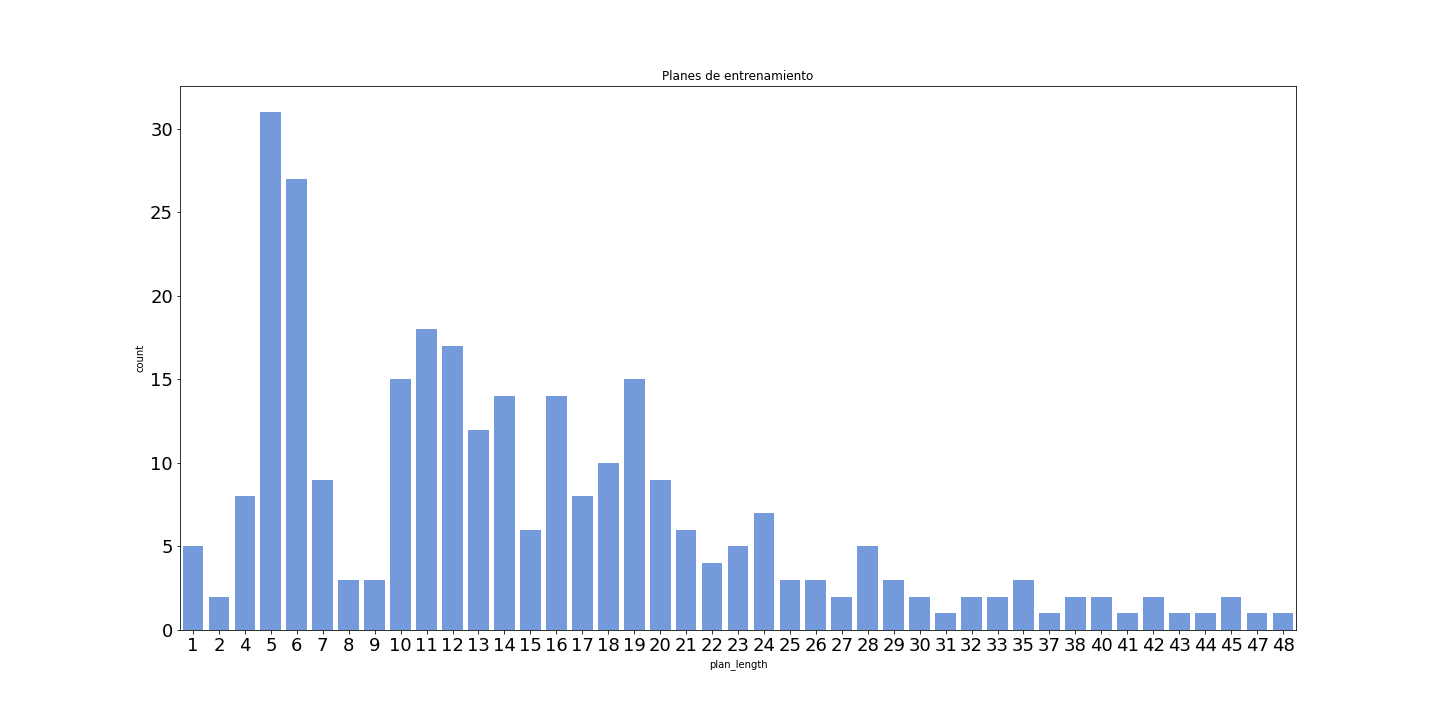
\includegraphics[width=\linewidth]{figures/plan_length_distplot_train.png}
        \caption{Planes relajados de entrenamiento}
        \label{fig:plan-length-distplot-train}
    \end{subfigure}
    \begin{subfigure}[b]{\textwidth}
        \centering
        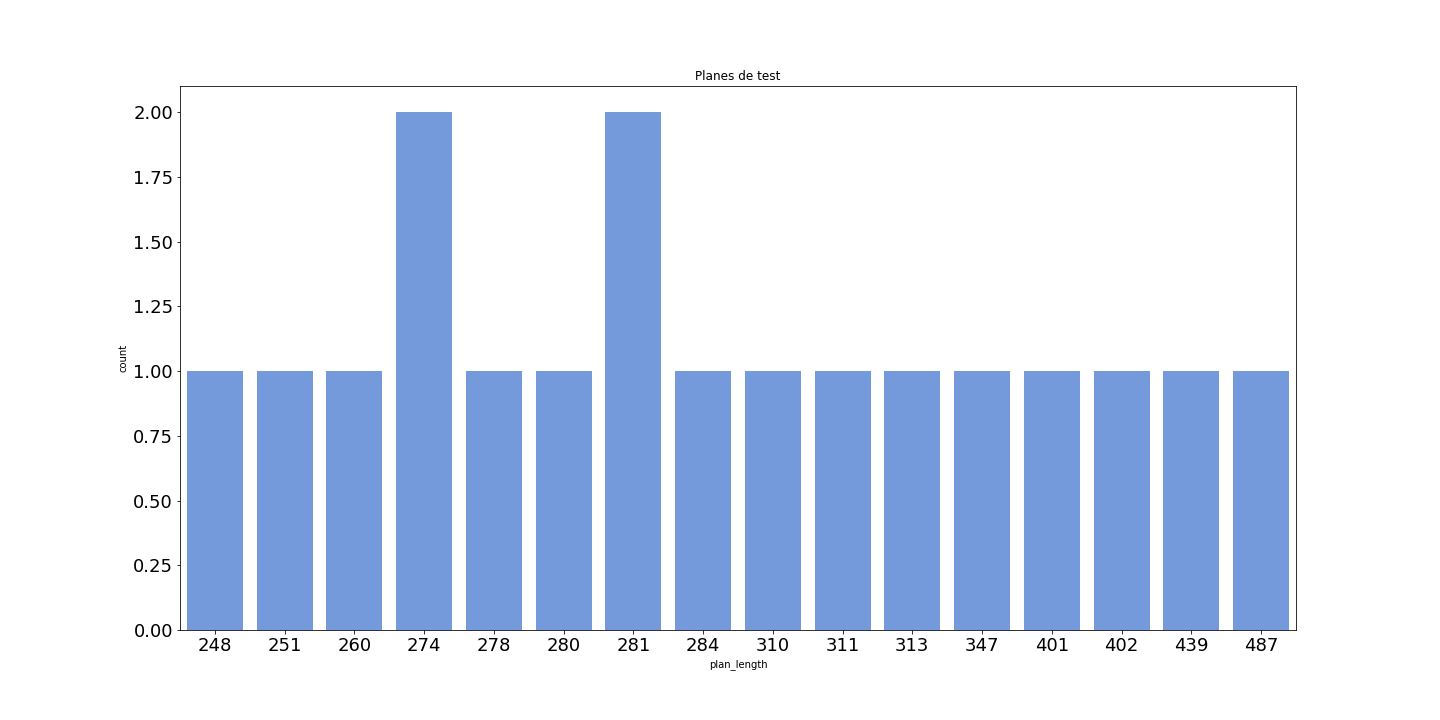
\includegraphics[width=\linewidth]{figures/plan_length_distplot_test.png}
        \caption{Planes relajados de test}
        \label{fig:plan-length-distplot-test}
    \end{subfigure}
    \caption{Distribución del largo de planes relajados}
    \label{fig:plan-length-distplot}
\end{figure}

La figura \ref{fig:window_example} muestra un ejemplo para una ventana de tamaño
3 y un paso de tamaño 2. Algo a notar de este ejemplo es que si la última
ventana generada no contiene la cantidad necesaria de acciones para generar una
ventana completa, se agregan palabras vacías hasta completar el largo restante.
Es importante también mencionar que ahora el tamaño de la matriz de entrenamiento
depende del largo de los planes relajados. En general, para una cantidad de
ventanas generadas $W$, good operators $N$, y bad operators $M$. Los ejemplos
generados son $W \times N \times M$. Por ejemplo, si para el plan relajado de la
figura \ref{fig:window_example}, se tienen 300 good operators y 1000 bad
operators. La cantidad de filas para ese problema es equivalente a $900000$
entradas. Esto es mucho peor para los problemas de test. Es por esto mismo que
no se pudieron generar muchos bad operators para estos problemas en la sección
\ref{method:data_generation}.

Una pregunta que queda por resolver es el valor de la etiqueta. Antes de incluir
las ventanas, nos interesaba determinar la probabilidad de que una acción sea
relevante para el plan real dado su plan relajado. Al utilizar las ventanas de
contexto, la pregunta es ligeramente distinta. Para este caso, nos interesa
determinar si la probabilidad de una acción es relevante para el plan real dada
una ventana del plan relajado. Si una acción es relevante en alguna ventana del
plan real entonces también lo es para el plan completo. Por lo tanto, para cada
uno de los planes relajados y acciones del conjunto de entrenamiento, propagamos
su etiqueta a su representación por partes.

\begin{figure}[t!]
    \centering
    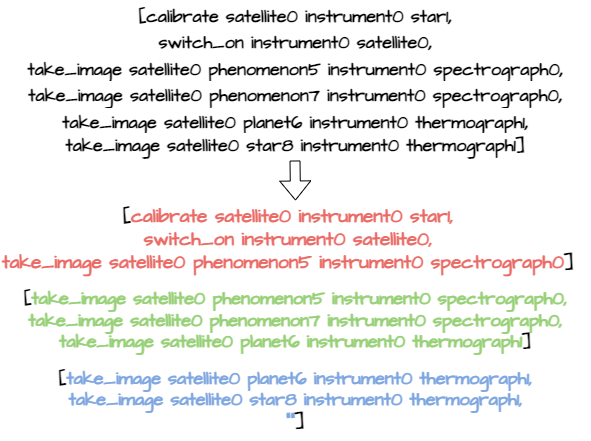
\includegraphics[width=\linewidth]{figures/window_example.png}
    \caption{Ejemplo de generación de ventanas para un plan relajado de largo 6.}
    \label{fig:window_example}
\end{figure}

Una vez generada las ventanas de planes relajados, obtenemos sus codificaciones
de manera ad-hoc o por word embeddings igual a como describimos en la sección
\ref{method:vectorization}.

\section{Selección de modelos}
\label{method:model_selection}

\subsection{Entrenamiento}

Una vez realizado el preprocesamiento estamos en condiciones de entrenar los
clasificadores que estudiamos en la sección \ref{lit:algorithms}. Los pares de
entrenamiento \{$(\vect{x}_1, y_1), ..., (\vect{x_n}, y_n)$\} para entrenar un
modelo de aprendizaje automático están compuestos por una representación de una
ventana perteneciente al plan relajado de un problema, y la representación de
una acción a estimar. Esto conforma el vector de características $\vect{x}_i$.
Las etiquetas reciben una codificación binaria de 1 o 0. Una etiqueta de 1
representa que la acción es relevante para el plan dado esa ventana del plan
relajado y una etiqueta de 0 indica lo contrario.

Para una configuración de parámetros, se entrena un clasificador utilizando
el conjunto de entrenamiento. A eso se agregan $k$ entrenamientos realizando
validación cruzada en $k$ grupos distintos. La única diferencia es que las
particiones son sobre los problemas de entrenamiento y no sobre el conjunto de
entrenamiento. Agrupar sobre este último puede llevar a que ventanas de un mismo
problema pertenezcan a grupos distintos y, por lo tanto, el problema esté
incompleto.

\subsection{Evaluación}

Una vez realizado los $k + 1$ entrenamientos del clasificador, deben ser
evaluados a partir del conjunto de test para obtener registro de las métricas
descriptas en la sección \ref{lit:metrics}. 

Inicialmente, es necesario generar las etiquetas, ventanas de planes relajados, y
codificación de los problemas de test. El conjunto de test resultante es dado
como entrada al modelo para obtener sus predicciones. Sin embargo, la evaluación
para nuestro problema es ligeramente distinta a la de un problema usual de
aprendizaje automático. Nuestro objetivo es estimar la probabilidad de que una
acción sea relevante para el plan real dado el plan relajado, pero el modelo
realizó sus predicciones a partir de ventanas del plan relajado. Es por eso que
la predicción final es la probabilidad máxima de todas las ventanas de un plan
relajado asociadas a una acción.

Ejemplo: Supongamos que tenemos la tabla de predicciones a nivel de ventanas de
plan relajado dado por la figura \ref{fig:window_example_evaluation}. Para la acción
\verb|switch on instrument0 satellite0|, la probabilidad máxima es la de la
ventana de color rojo. Por lo tanto, la predicción para esta acción dada el plan
relajado completo es la que predijo esa ventana.

\begin{figure}[t!]
    \centering
    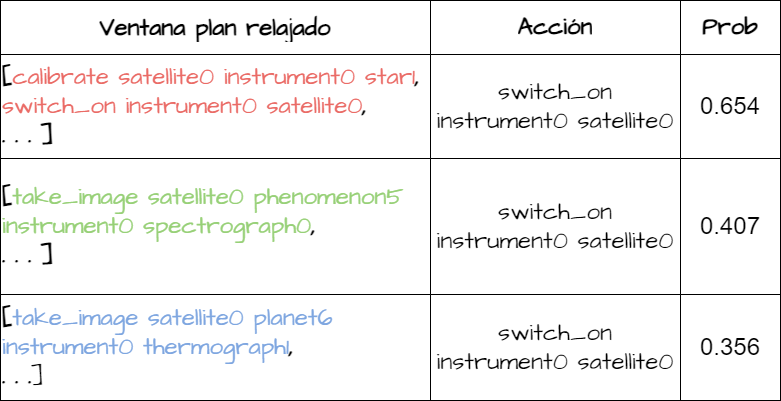
\includegraphics[width=\linewidth]{figures/aggregation_example.png}
    \caption{Ejemplo de evaluación por ventanas}
    \label{fig:window_example_evaluation}
\end{figure}

\section{Registro de resultados}

\subsection{Preservación de modelos, métricas, e imágenes}

Finalmente, evaluados los modelos, se almacenan los resultados (tanto métricas
como imágenes) de cada uno de los $k$ grupos, preservando únicamente los pesos y
parámetros del modelo entrenado con todo el conjunto de entrenamiento. Esto
último para aprovechar la totalidad de los ejemplos disponibles.

\subsection{Monitoreo y visualización}

Para el registro de métricas e imágenes se utilizó la librería \emph{MLFlow}.
 Esta herramienta permite el almacenamiento de datos y provee herramientas de
 visualización, registro de tiempos de ejecución de experimentos, comparación de
 experimentos, etc. Además de ser compatible con varias implementaciones de
 modelos. Algunas imágenes de las visualizaciones se pueden ver en la figura
 \ref{fig:mlflow-runs}.

 \begin{figure}[t!]
    \begin{subfigure}[b]{\textwidth}
        \centering
        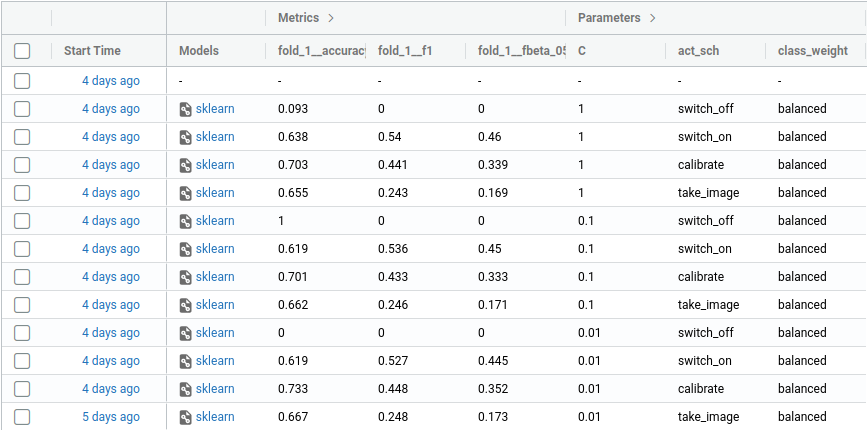
\includegraphics[width=\linewidth]{figures/runs_example_1.png}
        \caption{Tabla de resultados.}
    \end{subfigure}
    \hfill
    \begin{subfigure}[b]{\textwidth}
        \centering
        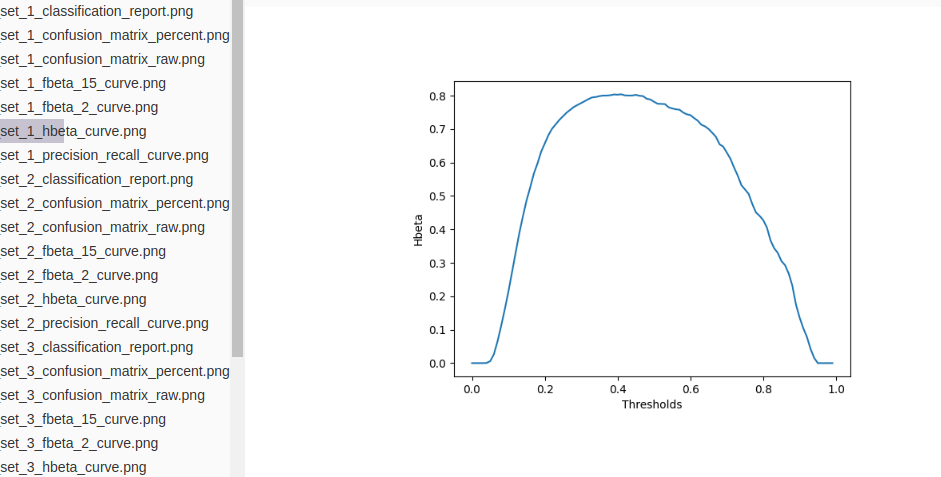
\includegraphics[width=\linewidth]{figures/runs_example_2.png}
        \caption{Visualización de gráficos.}
    \end{subfigure}
    \caption{Visualización de resultados desde MLFlow.}
    \label{fig:mlflow-runs}
\end{figure}

\subsection{Adaptación de modelos y transformadores}

En las secciones \ref{method:preprocessing}, y \ref{method:model_selection} se
puso mucho énfasis en la generación de los datos de esta tesis, así como los
pasos de exploración, preprocesamiento, entrenamiento y evaluación. Cada una de
estas etapas requirieron:

\begin{enumerate}
    \item Generación de especificaciones de problemas del dominio Satellite.
    \item Extracción de planes relajados, acciones instanciadas, y soluciones de
    los problemas a partir del planificador de Fast Downward.
    \item Separación en problemas de entrenamiento y test.
    \item Almacenamiento y preservación en una base de datos.
    \item Generación de conjuntos de entrenamiento y test.
    \item Transformación de los conjuntos de entrenamiento utilizando ventanas
    de planes relajados.
    \item Codificación de ventanas y acciones.
    \item Entrenamiento.
    \item Evaluación.
    \item Registro de resultados.
\end{enumerate}

Para la implementación de estos pasos se utilizó como lenguaje de programación
\emph{Python}. No obstante las librerías y herramientas principales requirieron
ser adaptadas a una interfaz común de tal manera que puedan ejecutarse de manera
sistemática. Esto se debió a que cada herramienta sigue sus propias convenciones.
Por ejemplo, la extracción de datos y lectura de archivos necesitó de librerías
que trabajen sobre el sistema de archivos, la persistencia de datos fue por
medio de \emph{SQL}, las consultas de bases de datos fueron realizadas por medio
del ORM \emph{SqlAlchemy}, las etapas de preprocesamiento en mayor parte fueron
con herramientas de \emph{Numpy} y \emph{Pandas}. La regresión logística y
XGBoost proveían una interfaz a través de \emph{Scikit-learn}, pero las redes
neuronales fueron implementadas en \emph{Pytorch}. La validación cruzada,
evaluación, y obtención de métricas también se hicieron con \emph{Scikit-learn}.
Y el registro de datos con \emph{MLflow}. Al momento de usar estas librerías
claramente fue necesario implementar una interfaz en común que minimice su
acoplamiento, este fue también uno de los desafíos de este trabajo.
    \chapter{Experimentos y resultados}
\label{ch:results}

En este capítulo presentaremos los experimentos principales realizados a partir
de lo desarrollado en el capítulo \ref{ch:method}. Entrenaremos 2 grupos de
modelos predictivos. Un grupo con una codificación ad-hoc, y otro grupo con una
codificación por word embeddings. Los vectores de características tendrán como
información una ventana del plan relajado y una acción. Se destacarán aquellos
modelos que presenten mejores resultados en validación cruzada y sobre ejemplos
del conjunto de test. Para aquellos modelos que tuvieron un mal desempeño,
mencionaremos algunas de las posibles causas.

Por otro lado se entrenarán los 3 algoritmos de clasificación vistos en el
capítulo \ref{ch:lit_ml}, \emph{XGBoost}, \emph{regresión logística}, y
\emph{perceptrón multicapa}. Los conjuntos de entrenamiento y de test son
divididos por esquemas de acción, entrenando un modelo por cada uno. Esto con el
fin de capturar la información significativa de un solo esquema por modelo. En
resumen, la estructura de nuestros experimentos para ambos grupos es la
siguiente:

\begin{itemize}
    \item Codificación ad-hoc o por word embeddings:
    \begin{itemize}
        \item Regresión logistica:
        \begin{itemize}
            \item \verb|take_image|
            \item \verb|turn_to|
            \item \verb|calibrate|
            \item \verb|switch_on|
            \item \verb|switch_off|
        \end{itemize}
        \item XGBoost:
        \begin{itemize}
            \item \verb|take_image|
            \item \verb|turn_to|
            \item \verb|calibrate|
            \item \verb|switch_on|
            \item \verb|switch_off|
        \end{itemize}
        \item Redes neuronales:
        \begin{itemize}
            \item \verb|take_image|
            \item \verb|turn_to|
            \item \verb|calibrate|
            \item \verb|switch_on|
            \item \verb|switch_off|
        \end{itemize}
    \end{itemize}
\end{itemize}

Esto es un total de 15 modelos por grupo. Para los mejores modelos, se
calcularon los tiempos de predicción con el fin de determinar si es viable
realizar grounding heurístico con estos modelos en el algoritmo de Fast
Downward.

Por último, mencionaremos otros experimentos que se trabajaron durante la tesis,
que a pesar de no lograr el resultado que esperábamos, fueron muy importantes
para guiar futuros experimentos.

\section{Modelos predictivos por word embeddings}
\label{exp:ad-hoc}

\subsection{Configuración del experimento}

En primer lugar, se necesito asignar la configuración para la construcción de
las ventanas y planes relajados.  Observamos que por lo general los planes
relajados del conjunto de entrenamiento suelen tener entre $3$ a $10$ acciones.
Nuestro algoritmo debe ser capaz de generalizar para ejemplos de entrenamientos
no antes visto, por lo que el preprocesamiento que realicemos sobre estos datos
debe ser orientado a reducir las discrepancias entre un ejemplo nuevo y los que
fueron utilizados en la etapa de entrenamiento. Como el largo de los planes
relajados de los problemas de test es por encima de los cientos de acciones,
generamos ventanas que aproximen en en tamaño a los planes relajados de los
problemas de entrenamiento. Es por ello, que optamos por un paso y tamaño de
ventana de $3$.

Para el entrenamiento de los clasificadores, se realizó una búsqueda de
hiper-parámetros cuya métrica a optimizar es $H_{\beta}$ con $\beta = 1.5$. Dado
que en nuestro problema es más importante predecir correctamente todas las
acciones relevantes, optamos por priorizar la taza de verdaderos positivos sobre
la taza de verdaderos negativos. Es decir, buscamos que el clasificador sea
penalizado si no logra predecir todas las acciones relevantes para obtener un
plan, y si no logra filtrar una cantidad aceptable de acciones no relevantes.

Recordemos que para evaluar los modelos, generamos las predicciones a nivel de
ventana de plan relajado y acción. No obstante, buscamos predecir si una acción
es relevante dada la información del plan relajado completo, por lo que es
necesario agrupar las predicciones que cada ventana realizó sobre esa acción.
Por ejemplo, supongamos que tenemos $M$ ventanas de un plan relajado $\vec{a}$
de una tarea $\Pi$ y se busca determinar la probabilidad de una acción $a'$ dado
$\vec{a}$. El modelo de aprendizaje automático propuesto realiza $M$
predicciones para $a'$ dado las $M$ ventanas de $\vec{a}$ donde cada estimación
es una probabilidad. En lugar de evaluar el modelo con las $M$ predicciones, las
agrupamos para obtener solo una. Para este experimento, seleccionamos el máximo
de las $M$ probabilidades. Notar que bajo esta decisión, una probabilidad baja
significa que para todas las ventanas del plan relajado, el planificador le
asignó una baja probabilidad a $a'$, mientras que una probabilidad alta requiere
que por lo menos una ventana del plan relajado haya provisto la información
necesaria para considerar relevante a $a'$.

Por último, los algoritmos presentados en el capítulo \ref{ch:lit_ml}
implementan una solución genérica de los métodos de aprendizaje. Por lo que se
requiere especificar como van a estar configurados antes de empezar el proceso
de entrenamiento. La siguiente lista de parámetros muestra aquellos que fueron
utilizados para cada algoritmo en este experimento:

\begin{conditions}
\emph{Nombre\ del\ modelo} & \verb|Regresión logística| \\
\emph{penalty} & \verb|[elasticnet]| \\
\emph{C} & \verb|[1, 0.1, 0.01]| \\
\emph{class\_weight} & \verb|[balanced]|  \\
\emph{solver} & \verb|[saga]|  \\
\emph{max\_iter} & \verb|[1000 10000]| \\
\emph{random\_state} & \verb|[0]| \\
\emph{l1\_ratio} & \verb|[0, 1]|
\end{conditions}

\begin{conditions}
\emph{Nombre\ del\ modelo} & \verb|XGBoost| \\
\emph{objective} & \verb|[binary:logistic]| \\
\emph{n\_estimators} & \verb|[500, 1000]| \\
\emph{gamma} & \verb|[0.001, 1]| \\
\emph{max\_depth} & \verb|[10, 20]| \\
\emph{alpha} & \verb|[0.001, 1]| \\
\emph{lambda} & \verb|[0.001, 1]| \\
\emph{booster} & \verb|[gbtree]| \\
\emph{colsample\_bytree} & \verb|[1]| \\
\emph{subsample} & \verb|[0.5]| \\
\emph{eval\_metric} & \verb|[logloss]| \\
\emph{use\_label\_encoder} & \verb|[false]| \\
\emph{random\_state} & \verb|[0]|
\end{conditions}

\begin{conditions}
\emph{Nombre\ del\ modelo} & \verb|PytorchNN| \\
\emph{h\_size} & \verb|[32, 64]| \\
\emph{n\_layers} & \verb|[2, 4, 8, 16]| \\
\emph{bn\_bool} & \verb|[False]| \\
\emph{p} & \verb|[0, 0.1]| \\
\emph{epochs} & \verb|[20]| \\
\emph{batch\_size} & \verb|[32]| \\
\emph{balanced} & \verb|[True]| \\
\emph{lr} & \verb|[0.001]| \\
\end{conditions}

Estos parámetros corresponden con la interfaz provista por las librerías de
\emph{Scikit-learn} y \emph{Pytorch} que implementan los algoritmos de
aprendizaje. Cada parámetro muestra una lista de 1 o más valores donde cada
elemento representa una posible asignación de ese parámetro. La cantidad de
configuraciones posibles de un modelo es igual al producto cartesiano de cada
una de las listas de los parámetros de un modelo. Por ejemplo para el caso de la
regresión logística, los parámetros \emph{C}, \emph{max\_iter}, y
\emph{l1\_ratio} tienen 3, 2, y 2 asignaciones respectivamente, el resto de
parámetros solo tiene una. Por lo tanto, hay un total de $3 \times 2 \times 2 =
12$ configuraciones del modelo.

Los parámetros que seleccionamos siempre buscaban plantear variantes en la
función de costo a optimizar, el tipo de optimizador, y métodos para evitar el
sobreajuste. En particular, seguimos como guía valores comunes que la comunidad
de aprendizaje automático suele utilizar para estos modelos,  la experiencia
transmitida por el ´boca a boca´, y conocimientos tanto del área de planning
como del funcionamiento interno de los modelos utilizados. 

En el caso de la regresión logística, los parámetros \emph{penalty},
\emph{l1\_ratio}, y \emph{C} permiten realizar variaciones en la regularización
de la función de costo, evitando que la norma del vector de pesos del modelo
crezca demasiado por sobreajuste. \emph{solver} indica el método de optimización
de la función de costo. \emph{max\_iter} es el número de iteraciones que
requiere el algoritmo para converger. Por último, \emph{class\_weight} permite
configurar el modelo de tal manera que balancee la cantidad de ejemplares
positivos y negativos del material de entrenamiento. Este último es importante
para nosotros ya que nuestro conjunto de entrenamiento está desbalanceado,
teniendo una mayor cantidad de good operators que de bad operators por problema.

XGBoost requiere que se le especifiquen la cantidad de árboles a ensamblar con
\emph{n\_estimators}, la fuerza del parámetro de regularización \emph{gamma}, y
la profundidad máxima de los árboles \emph{max\_depth}. \emph{objetive} indica
la función objetivo a optimizar, en este caso la misma función de costo que una
regresión logística. \emph{booster} permite seleccionar variantes del método
iterativo de boosting explicado en el capítulo \ref{alg:xgboost}. Por último
\emph{colsample\_bytre} y \emph{subsample} permiten tomar una muestra con
reposición de las filas o columnas en la confección de un árbol en el ensemble
con el proposito de reducir el sobreajuste.

La red neuronal necesita del número de neuronas para todas las capas
\emph{h\_size}, la cantidad de capas ocultas \emph{n\_layers}, si los vectores
de entrada son normalizados \emph{bn\_bool}, y la probabilidad  \emph{p} de
apagar momentáneamente neuronas de la red de manera aleatoria.

Por cada posible asignación obtenemos aquella que mejor se comporte con el
conjunto de test. Recordemos que nuestro objetivo es encontrar modelos que se
pueda utilizar para algún esquema de acción. De un total de 5 esquemas de acción
en el dominio \emph{Satellite}, el mejor caso sería encontrar 5 modelos que den
buenos resultados en esos esquemas.

\subsection{Resultados: take\_image}

Empecemos por el esquema de acción \verb|take_image| con el cual obtuvimos
mejores resultados. De los 3 modelos regresión logística (LGR), xgboost (XGB), y
redes neuronales (NN), el que mejor comportamiento que obtuvimos fue con la
regresión logística. 

\subsubsection{Performance en validación cruzada}

La figura \ref{fig:takeimage-bestmodel-distplot} muestra la distribución de las
predicciones en validación cruzada para la mejor configuración de parámetros de
LGR.


\begin{figure}
    \begin{subfigure}[b]{\textwidth}
        \centering
        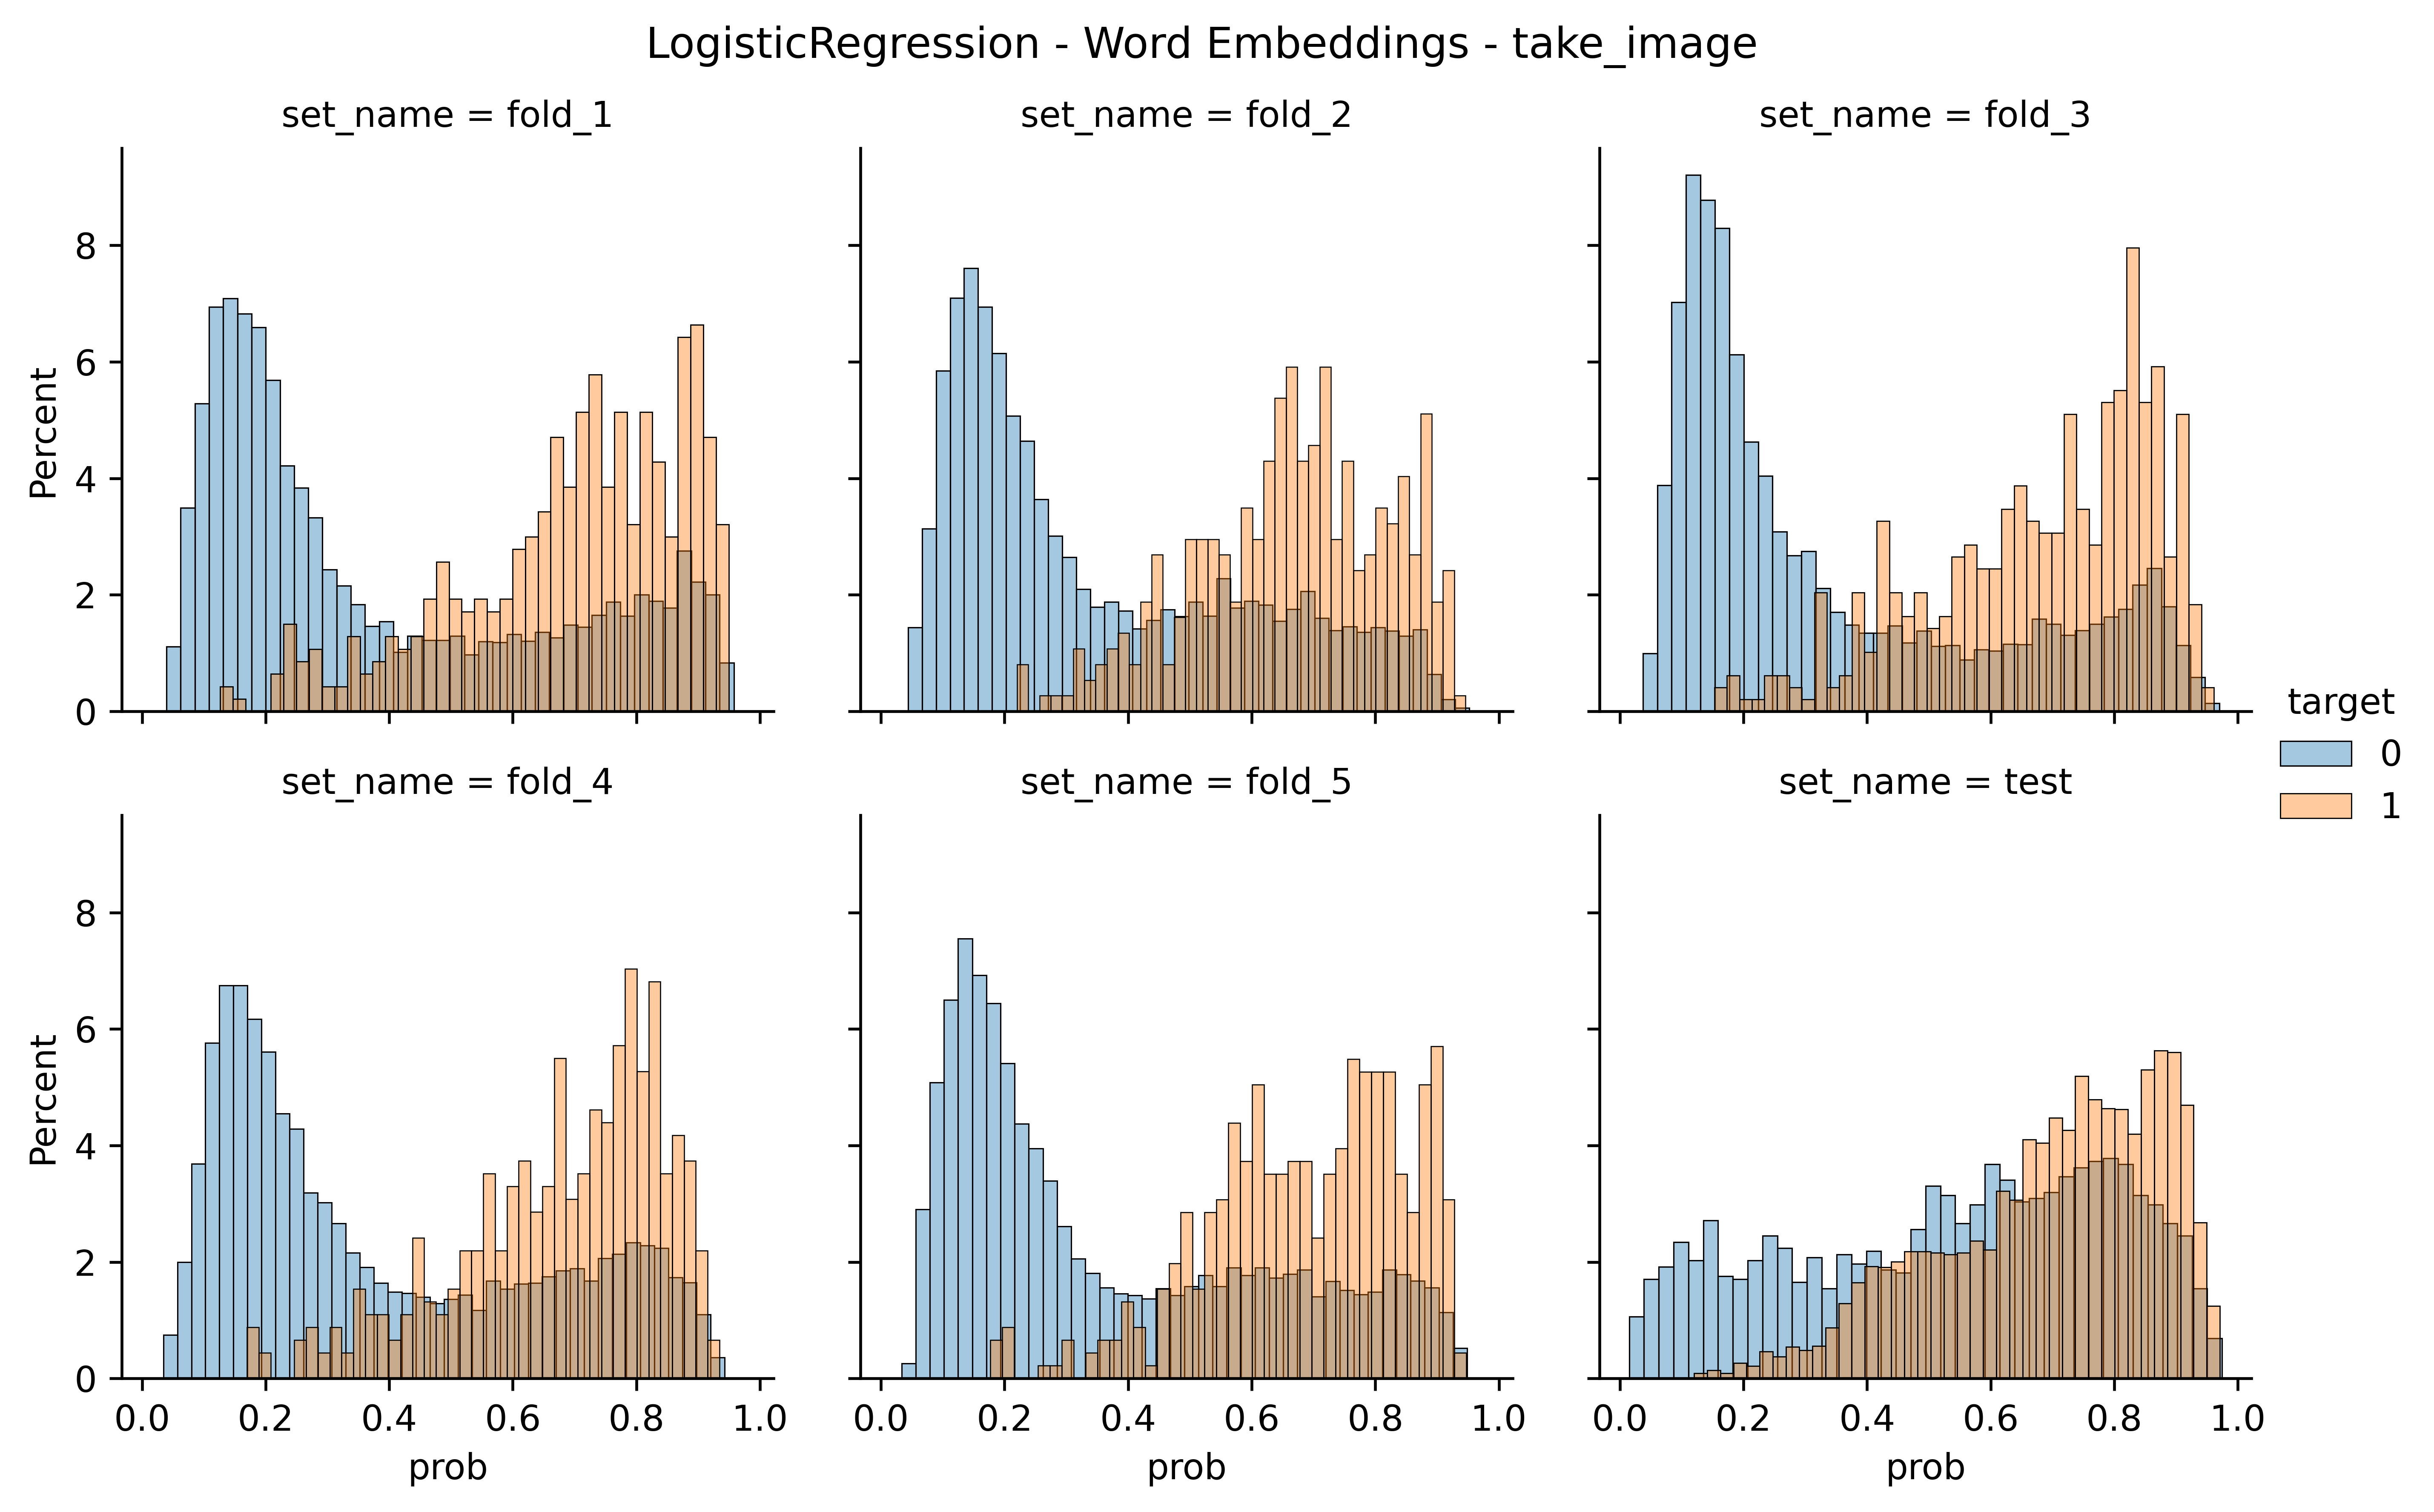
\includegraphics[width=\linewidth]{figures/results/word_embeddings/lgr/take_image/lgr__distplot.png}
        \caption{Distribución de predicciones en validación cruzada y el conjunto de test.}
        \label{fig:takeimage-bestmodel-distplot}
    \end{subfigure}
    \hfill
    \begin{subfigure}[b]{\textwidth}
    \minipage{0.32\textwidth}
      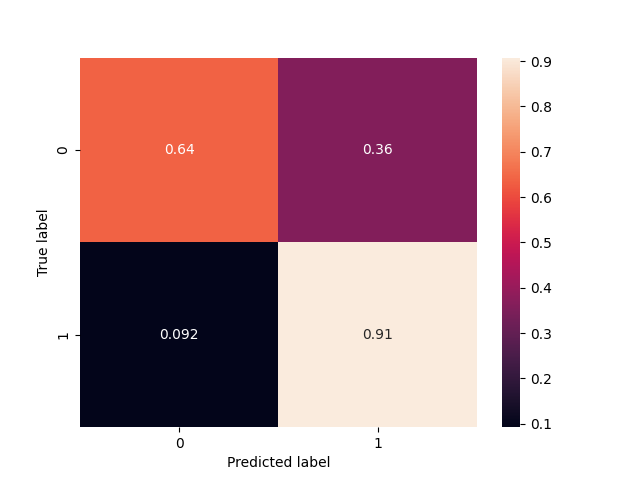
\includegraphics[width=\linewidth]{figures/results/word_embeddings/lgr/take_image/lgr_set_1_confusion_matrix_percent.png}
    \endminipage\hfill
    \minipage{0.32\textwidth}
      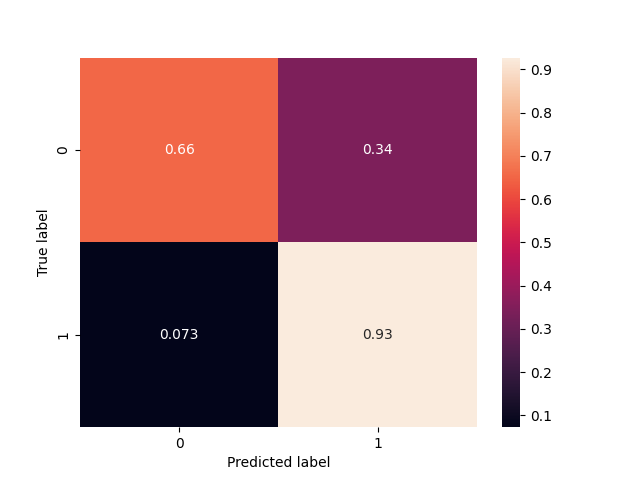
\includegraphics[width=\linewidth]{figures/results/word_embeddings/lgr/take_image/lgr_set_2_confusion_matrix_percent.png}
    \endminipage\hfill \minipage{0.32\textwidth}%
      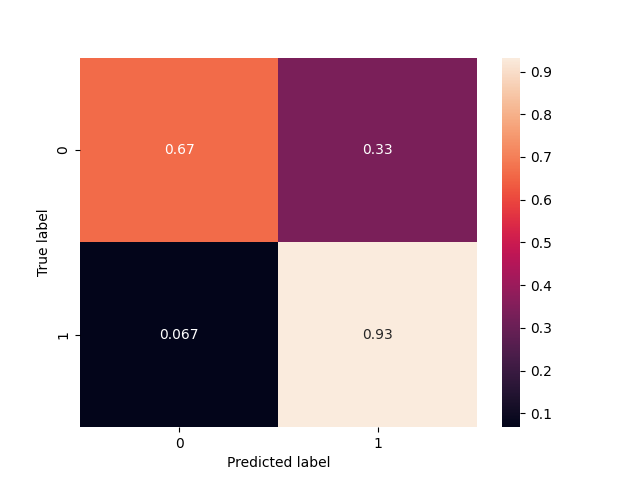
\includegraphics[width=\linewidth]{figures/results/word_embeddings/lgr/take_image/lgr_set_3_confusion_matrix_percent.png}
    \endminipage
    
    \medskip
    
    \minipage{0.32\textwidth}
      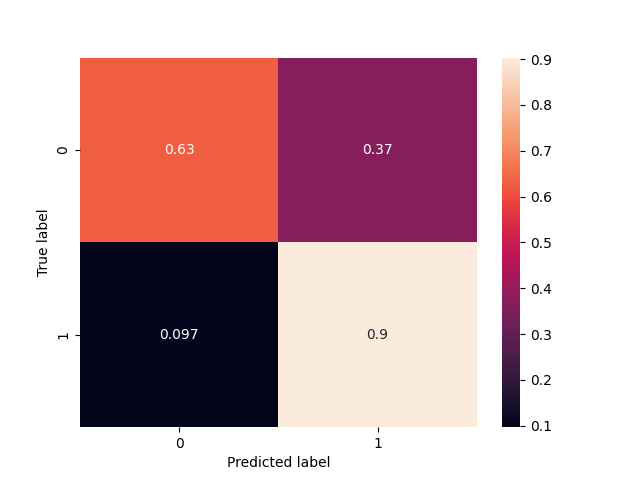
\includegraphics[width=\linewidth]{figures/results/word_embeddings/lgr/take_image/lgr_set_4_confusion_matrix_percent.png}
    \endminipage\hfill
    \minipage{0.32\textwidth}
      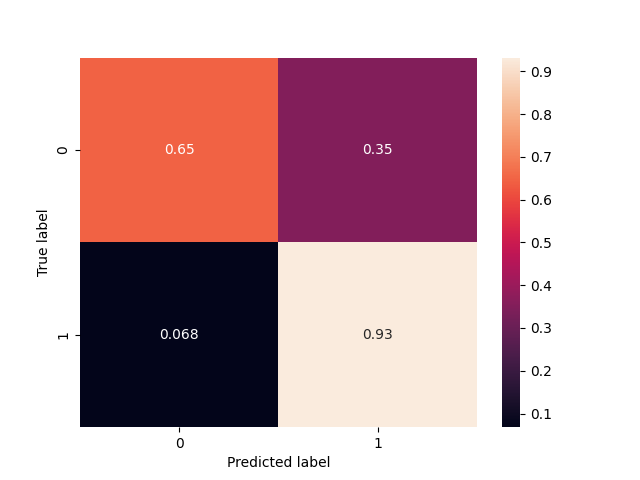
\includegraphics[width=\linewidth]{figures/results/word_embeddings/lgr/take_image/lgr_set_5_confusion_matrix_percent.png}
    \endminipage\hfill \minipage{0.32\textwidth}%
      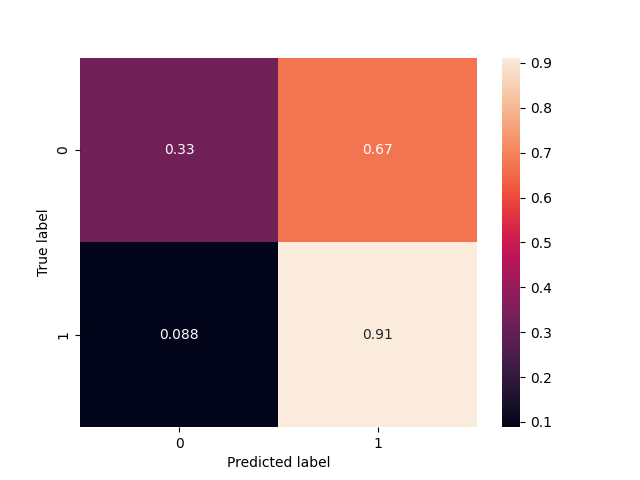
\includegraphics[width=\linewidth]{figures/results/word_embeddings/lgr/take_image/lgr_set_6_confusion_matrix_percent.png}
    \endminipage
    \caption{Matrices de confusión en validación cruzada y el conjunto de test}
    \label{fig:takeimage-bestmodel-cm}
    \end{subfigure}
    \caption{Resultados del modelo de regresión logística con codificación por word embeddings y esquema de acción take\_image.}
    \label{fig:takeimage-bestmodel}
\end{figure}


La figura muestra dos histogramas independientes, el de la clase positiva, y el
de la clase negativa. Cada punto en el gráfico representa la probabilidad de una
acción dado su plan relajado (completo). Para ambos histogramas se genera una
cantidad $N$ de bins equidistantes en el rango [0, 1]. Luego, para cada bin $b$,
se muestra la cantidad de acciones que recibieron una probabilidad contenida en
$b$ divido el tamaño de la clase a la que pertenecen.

Para el histograma de la clase positiva, observamos que las acciones relevantes
(good operators) se agrupan en los bins con probabilidades entre $r=[0,6; 1]$.
Cada bin contiene entre el 2\% al 7\% de las acciones. Si sumamos los
porcentajes de cada uno de los bins en $r$, tendremos que más de la mitad de las
acciones se encuentran en $r$.

Por otro lado, el histograma de la clase negativa, muestra que más de la mitad
de las acciones no relevantes (bad operators) se agrupan en los bins con
probabilidades entre $[0;0.4]$.

Desde el punto de vista de grounding heurístico este es el comportamiento que
buscamos. El algoritmo almacenará en una cola de prioridades acciones tanto
relevantes como no relevantes con una probabilidad asociada, dándole prioridad a
las que tienen una mayor probabilidad. Si el modelo asigna a las acciones
relevantes una alta probabilidad entonces el proceso de grounding heurístico les
dará prioridad para su instanciación.

Notar que el objetivo de utilizar validación cruzada es variar el conjunto de
entrenamiento con el fin de determinar si el modelo de LGR es robusto ante
cambios, lo cual podemos decir que indudablemente fue este el caso en las 5
particiones.

Si observamos la matriz de confusión del modelo por cada partición dada por la
figura \ref{fig:takeimage-bestmodel-cm}, podemos ver que en cada uno, más del
90\% de las acciones positivas se predicen como positivas, y más del 63\% de las
negativas se predicen como negativas. La función de decisión se obtiene a partir
del cálculo de $H_{1.5}$. Es decir, se computa $H_{1.5}$ para distintas
funciones de decisión con umbral en el intervalo [0, 1] y utilizamos aquel que
maximice $H_{1.5}$. 

\subsubsection{Performance en test}

Los resultados anteriores fueron sobre 5 particiones del conjunto de
entrenamiento donde una parte efectivamente se utilizaba para entrenar el modelo
y otra para su evaluación. Sin embargo, lo que buscamos es que esto mismo se
logre generalizar a problemas no instanciables. Por lo tanto, la evaluación
final la realizamos sobre el conjunto de test.

\begin{figure}
    \centering
    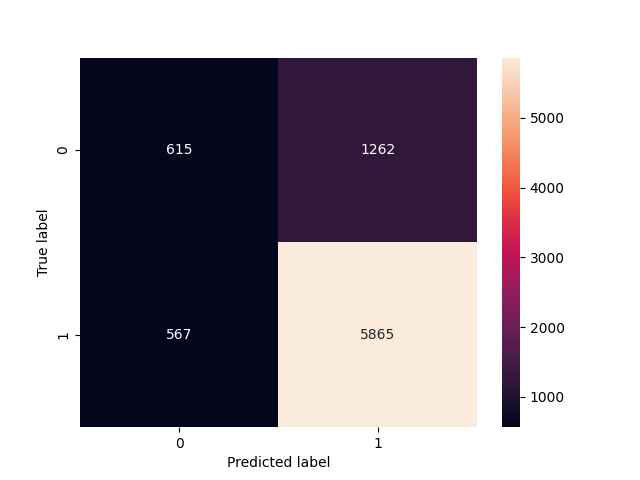
\includegraphics[scale=0.7]{figures/results/word_embeddings/lgr/take_image/lgr_set_6_confusion_matrix_raw.png}
    \caption{Matriz de confusión sin porcentajes del modelo de regresión logística con codificación por word embeddings y esquema de acción take\_image.}
    \label{fig:takeimage-bestmodel-cm-raw}
\end{figure}

La figura \ref{x} muestra nuevamente muestra un histograma de la probabilidad de
una acción dado su plan relajado. El caso de las acciones relevantes se sigue
manteniendo el comportamiento que vimos en validación cruzada lo cual es un buen
indicio ya que estarán en las primeras posiciones en la cola de prioridades en
grounding heurístico. Sin embargo, si observamos el histograma de acciones no
relevantes, se tiene que ahora a una gran parte de ellas se le asigna una alta
probabilidad. Estas acciones también serían ubicadas al comienzo de la cola de
prioridades y por lo tanto instanciadas. Si observamos la matriz de confusión en
\ref{x'}, la proporción de acciones relevantes se mantiene en un 91\%, mientras
que esta vez un 67\% de las no relevantes se filtran como positivas, cabe
recalcar que esta vez, el umbral de decisión en test es el promedio de los
umbrales obtenidos en validación cruzada. El objetivo era aprender un umbral que
sea lo más óptimo para predecir nuevos ejemplos, utilizando únicamente
información de los datos de entrenamiento. Podríamos haber utilizado un umbral
de decisión a partir de las etiquetas de test, no obstante tal predicción
representaría la performance máxima o ideal que podríamos obtener en test, y no
la que realmente estamos obteniendo con información del conjunto de
entrenamiento.

Por último, si observamos la matriz de confusión de la figura
\ref{fig:takeimage-bestmodel-cm-raw} del modelo LGR, pero esta vez sin
normalizar por porcentajes. Se puede ver que LGR tiende a predecir ligeramente
sobre la clase positiva, pero además es la mayoritaria en test para este
esquema. Esto sucede debido a como se generan los bad operators en los problemas
de test. Recordemos que estos no pueden obtenerse por Fast Downward por lo que
se generó una muestra aleatoria usando grounding cartesiano pero respetando los
tipos de las interfaces. Como solo se pudieron generar una cantidad de 5000 bad
operators por problema, y los planes en los problemas de test son de mayor
tamaño que los de entrenamiento, surgió este desbalance hacia la clase positiva.
No obstante, en una situación real, la cantidad de bad operators sería
nuevamente superior a la de good operators. Otro aspecto importante sobre la
generación de los bad operators es que podrían no ser alcanzables relajadamente,
y por lo tanto tener una distribución distinta a la que tenemos en el conjunto
de entrenamiento siendo una de las posibles causas del desempeño de LGR para la
clase negativa. Es decir, LGR fue entrenado para predecir, sobre acciones
alcanzables relajadamente, pero lo estamos evaluando sobre bad operators que no
lo son.

Por último, notar que precision y recall sobre la clase positiva es de 0.823, y
0.912, respectivamente. Si calculamos la métrica $F_{1.5}$ priorizando recall,
obtendriamos una performance de 0.8826 para LGR. Sin embargo, no es un buen
indicio de la correctitud del modelo en la clase negativa, como podemos ver en
el cuadro \ref{results:lgr-wb-calibrate}. En contraparte, si en lugar de
considerar $F_{1.5}$ utilizamos $H_{1.5}$ la performance es de 0.589 lo cual
al penalizar la baja en la taza de verdaderos negativos.

\begin{table}[h!]
\centering
\scalebox{0.9}{
 \begin{tabular}{|c || c | c | c | c | c | c |} 
 \hline
  Clase & Precisión & Recall & $H_{1.5}$ & $F_{1.5}$ & Umbral de decisión \\
 \hline
 Relevante & 0.823 & 0.912 & 0.589 & 0.8826 & 0.416 \\
 No relevante & 0.52 & 0.33 & 0.4081 & 0.3717 & 0.416 \\
 \hline
 \end{tabular}}
 \caption{Resultados por esquema de acción del mejor modelo con codificación por word embeddings.}
 \label{results:lgr-wb-calibrate}
\end{table}

\begin{figure}
    \centering
    \begin{subfigure}[b]{0.83\textwidth}
    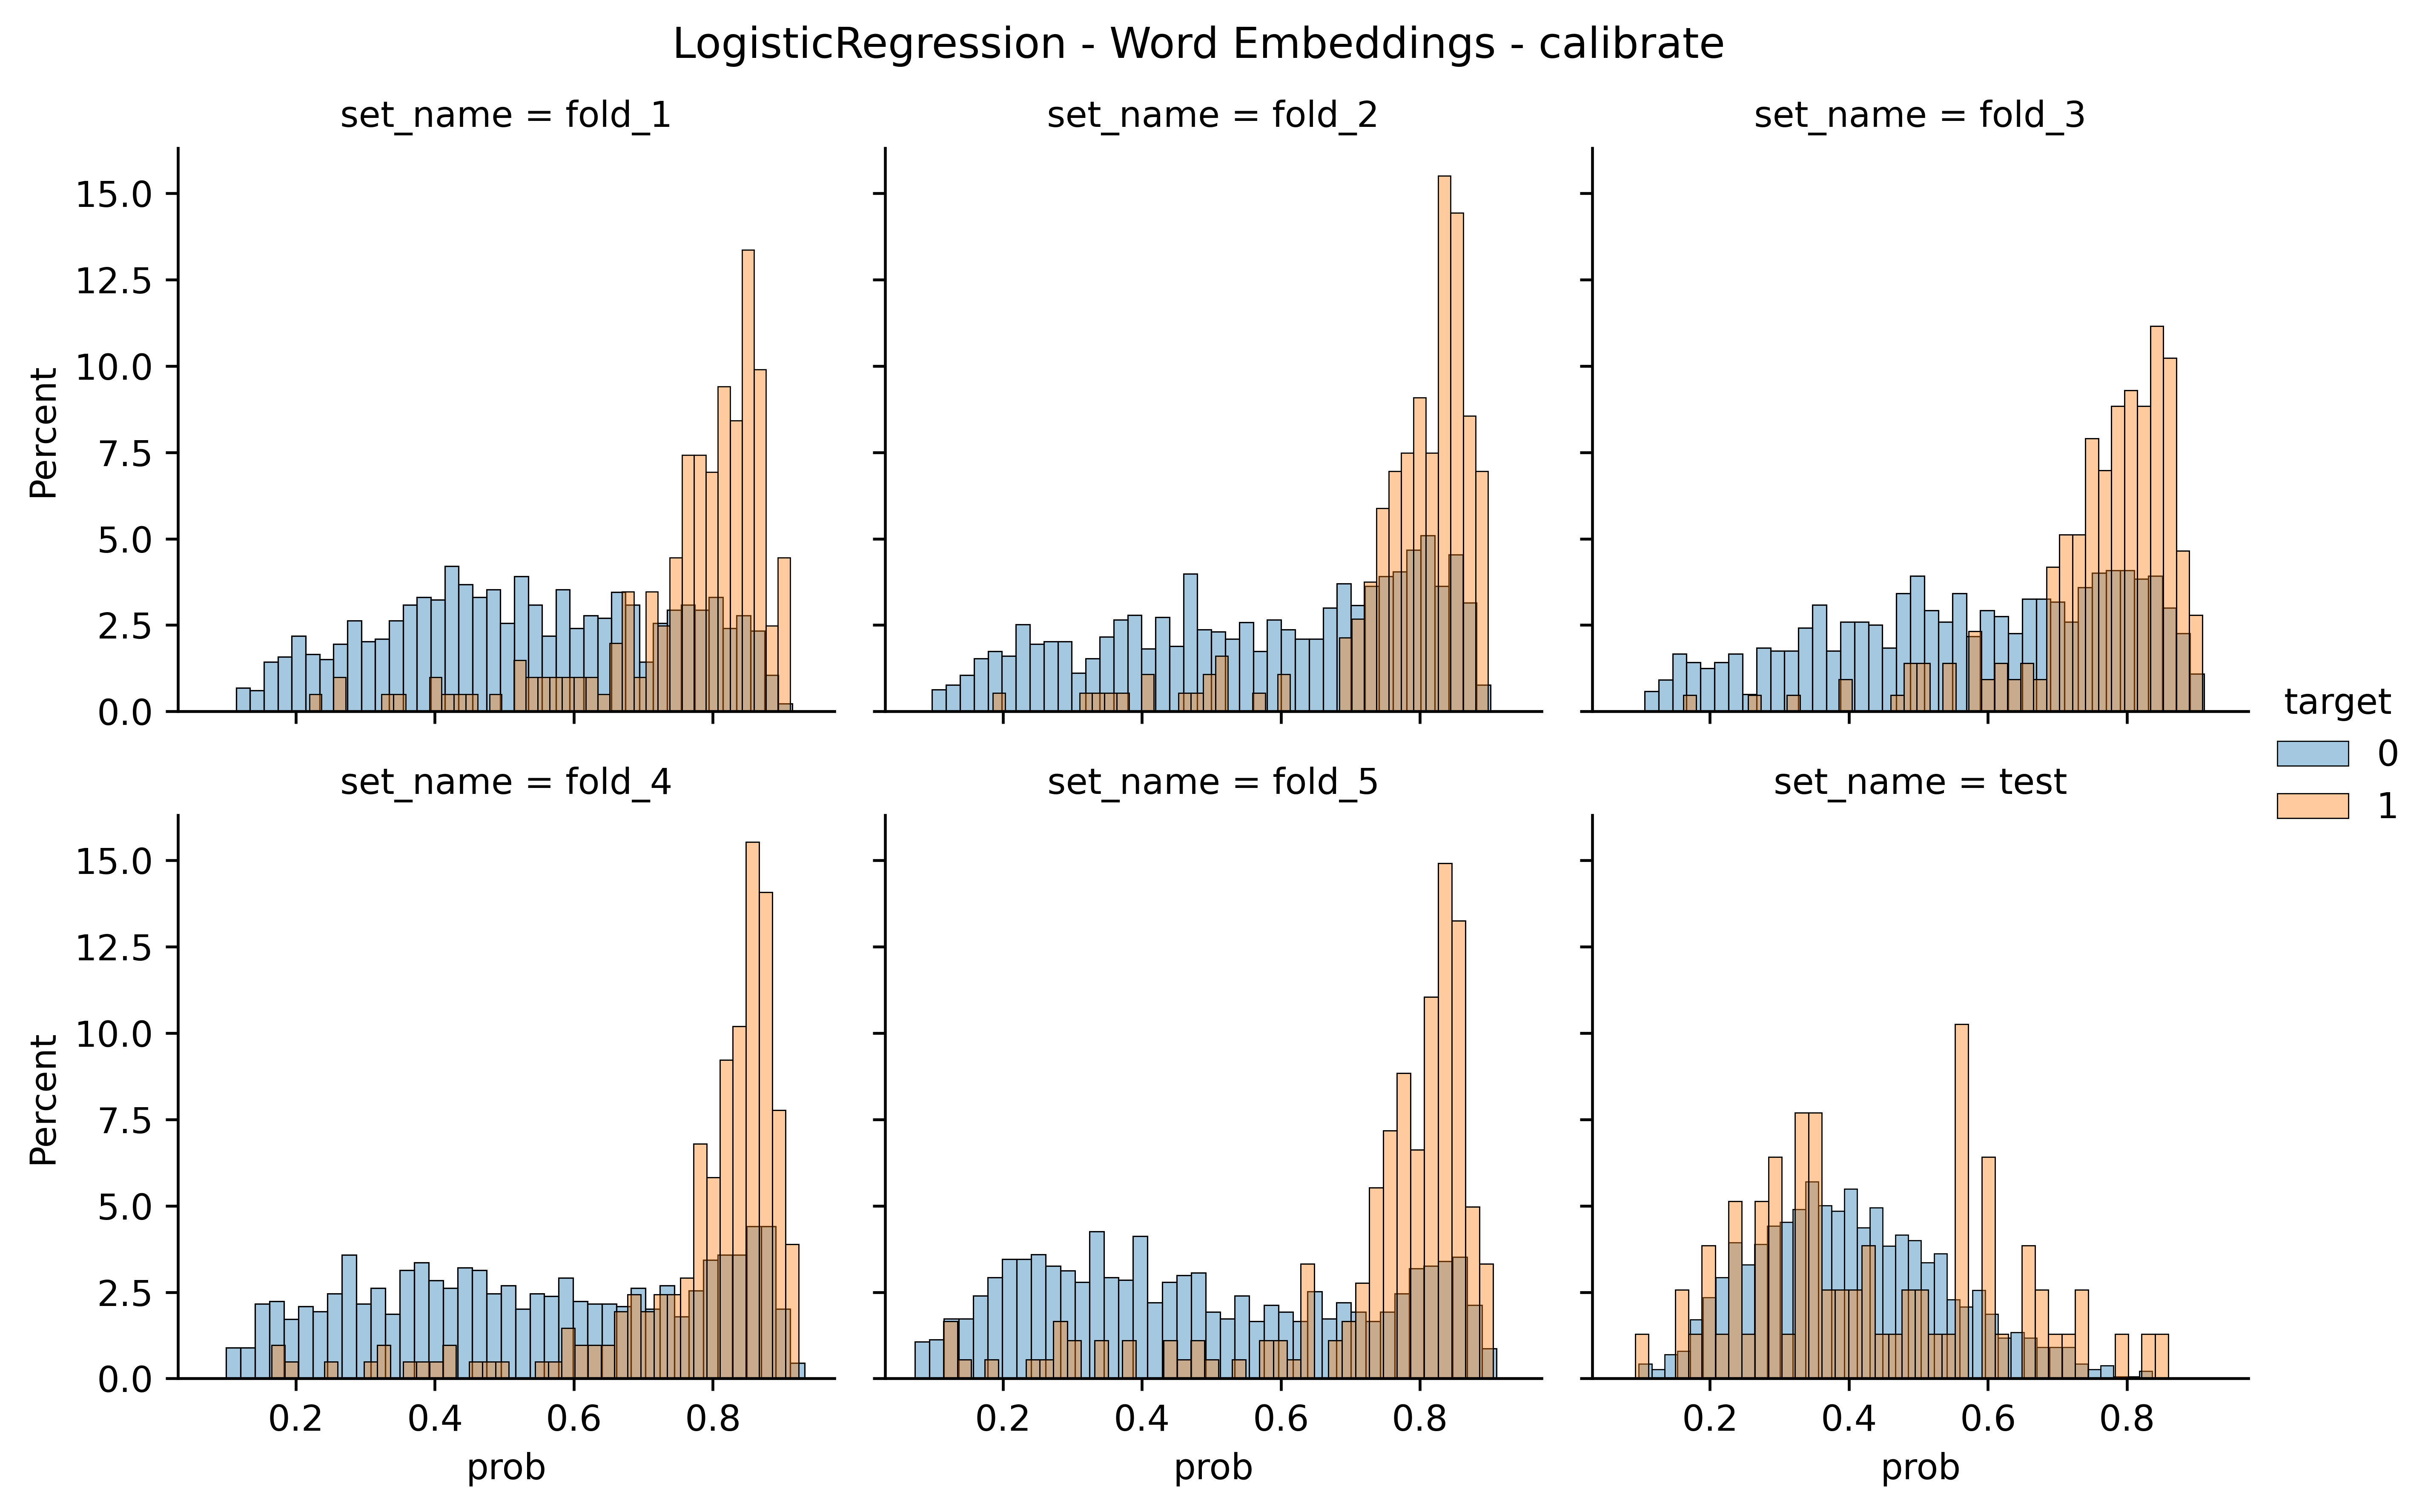
\includegraphics[width=\linewidth]{figures/results/word_embeddings/lgr/calibrate/calibrate__distplot.png}
    \end{subfigure}
    \hfill
    \centering
    \begin{subfigure}[b]{0.83\textwidth}
        \centering
        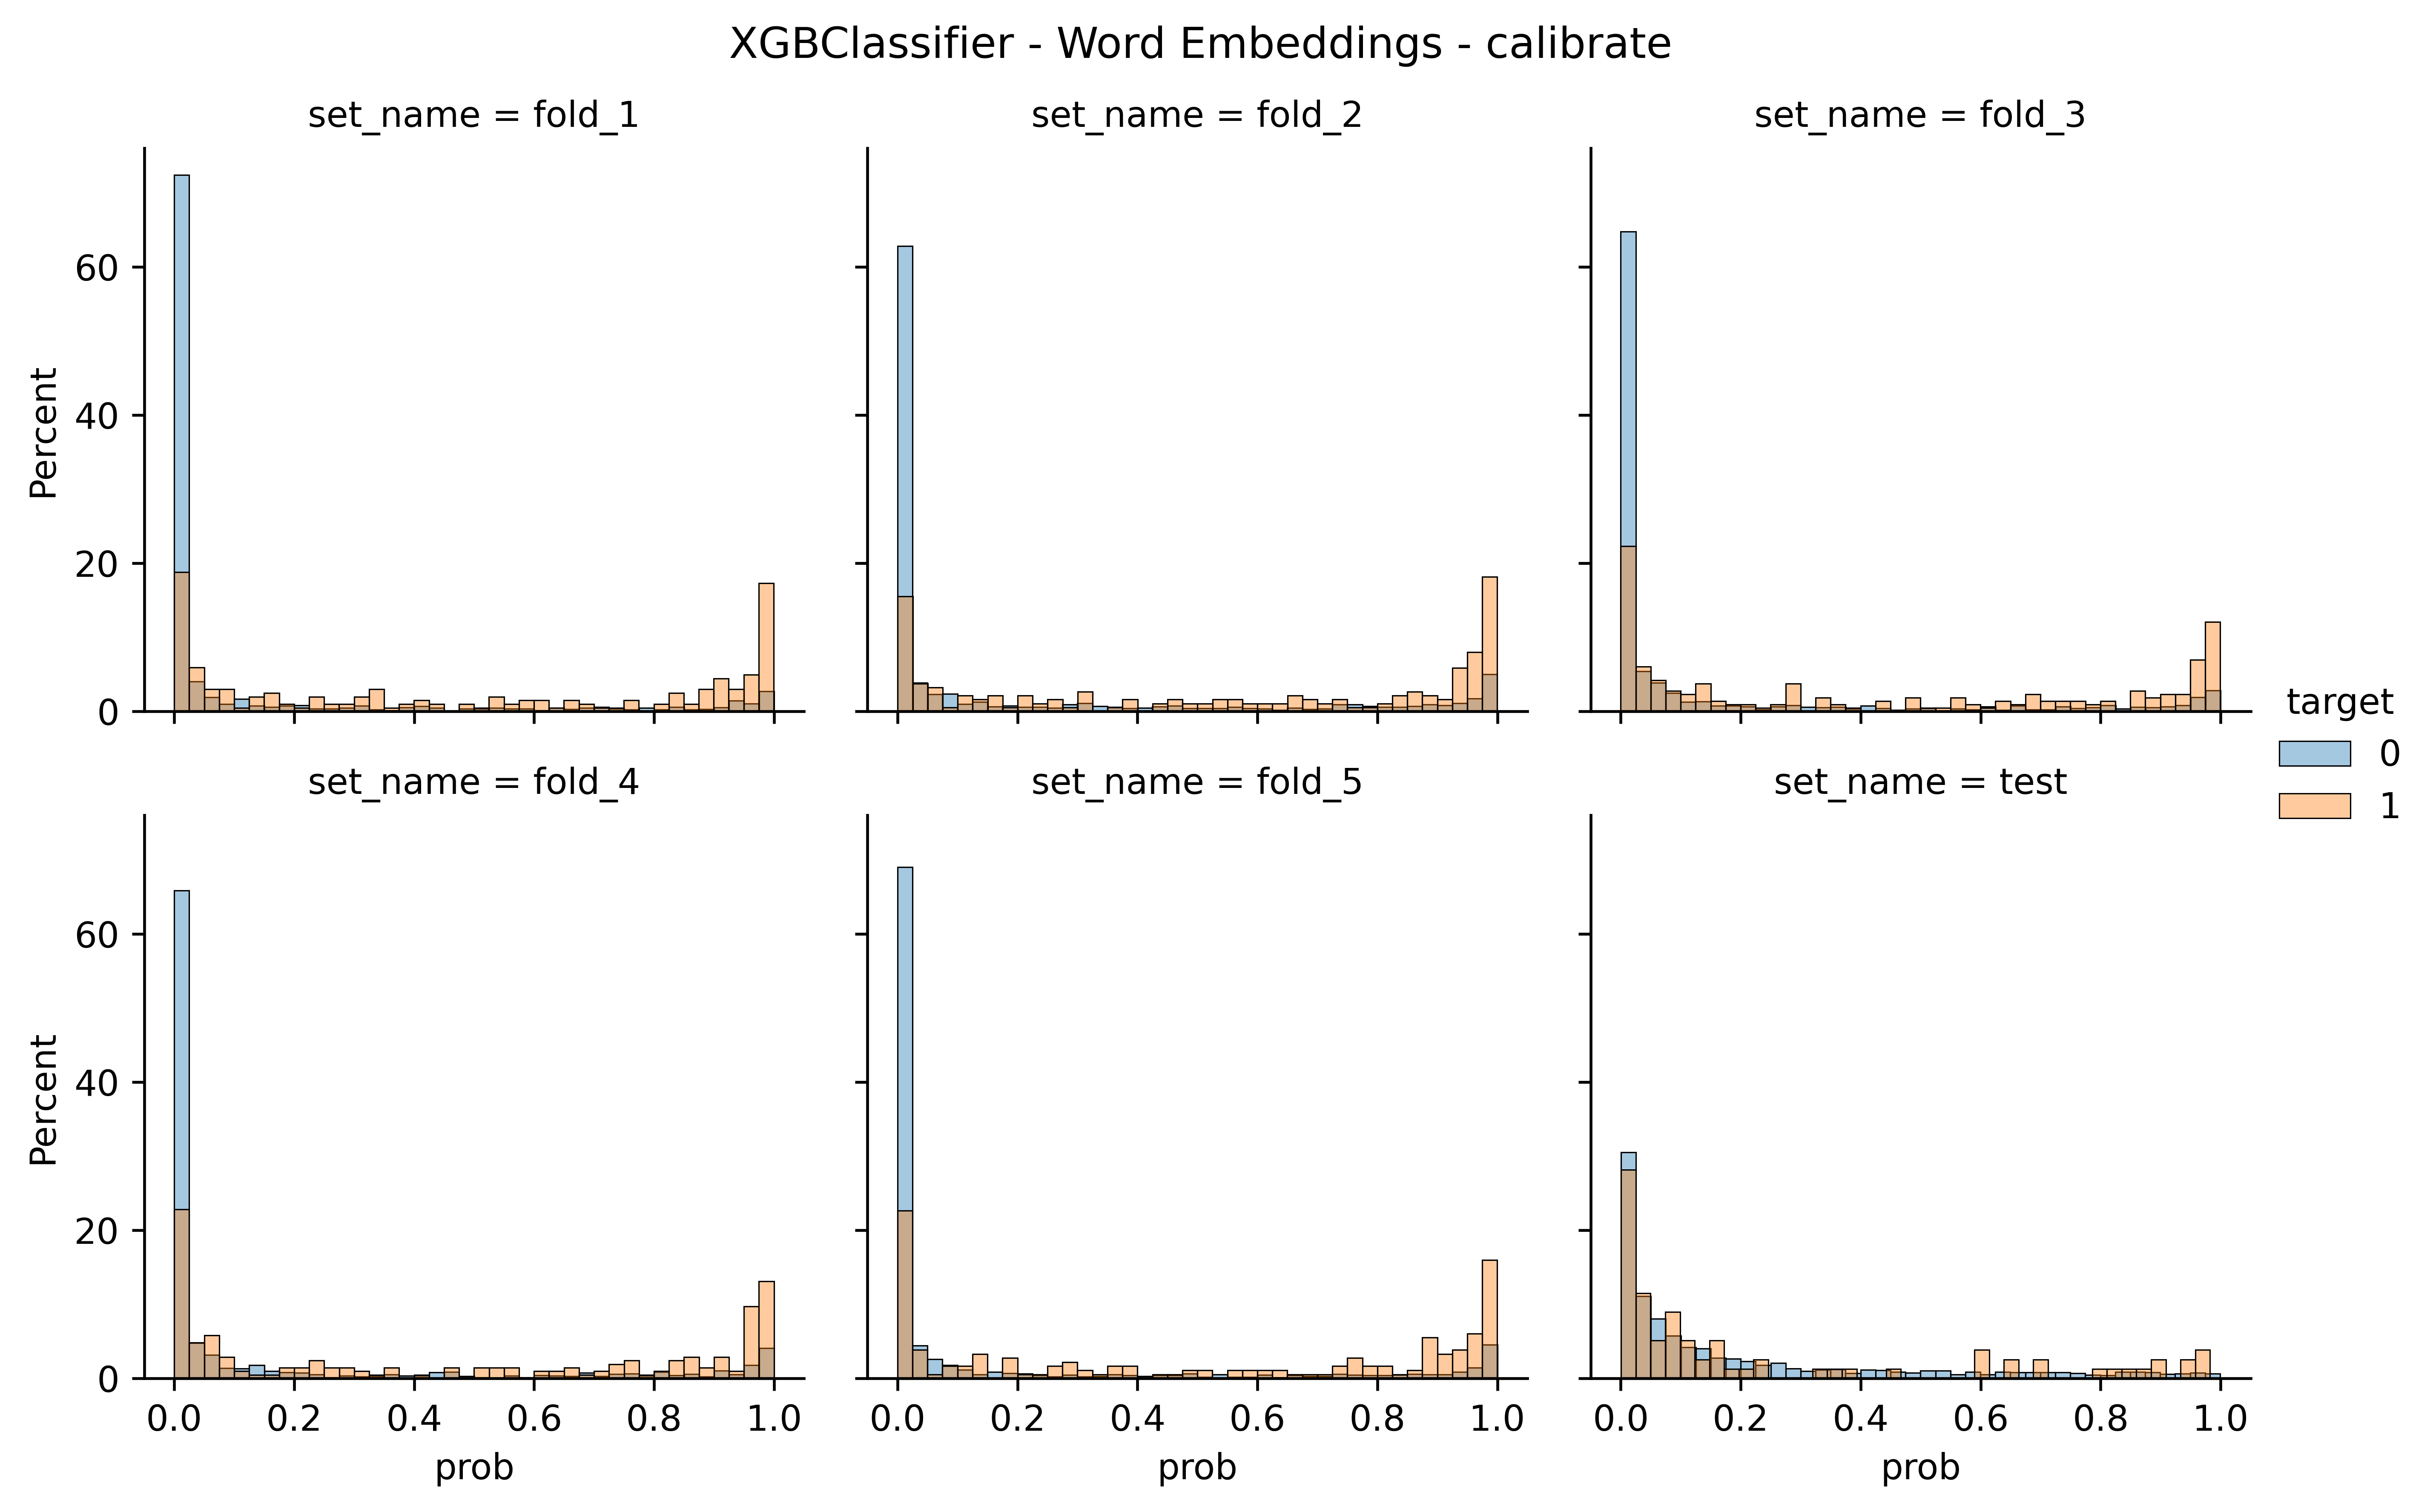
\includegraphics[width=\linewidth]{figures/results/word_embeddings/xgboost/calibrate/calibrate__distplot.png}
    \end{subfigure}
    \hfill
    \centering
    \begin{subfigure}[b]{0.83\textwidth}
        \centering
        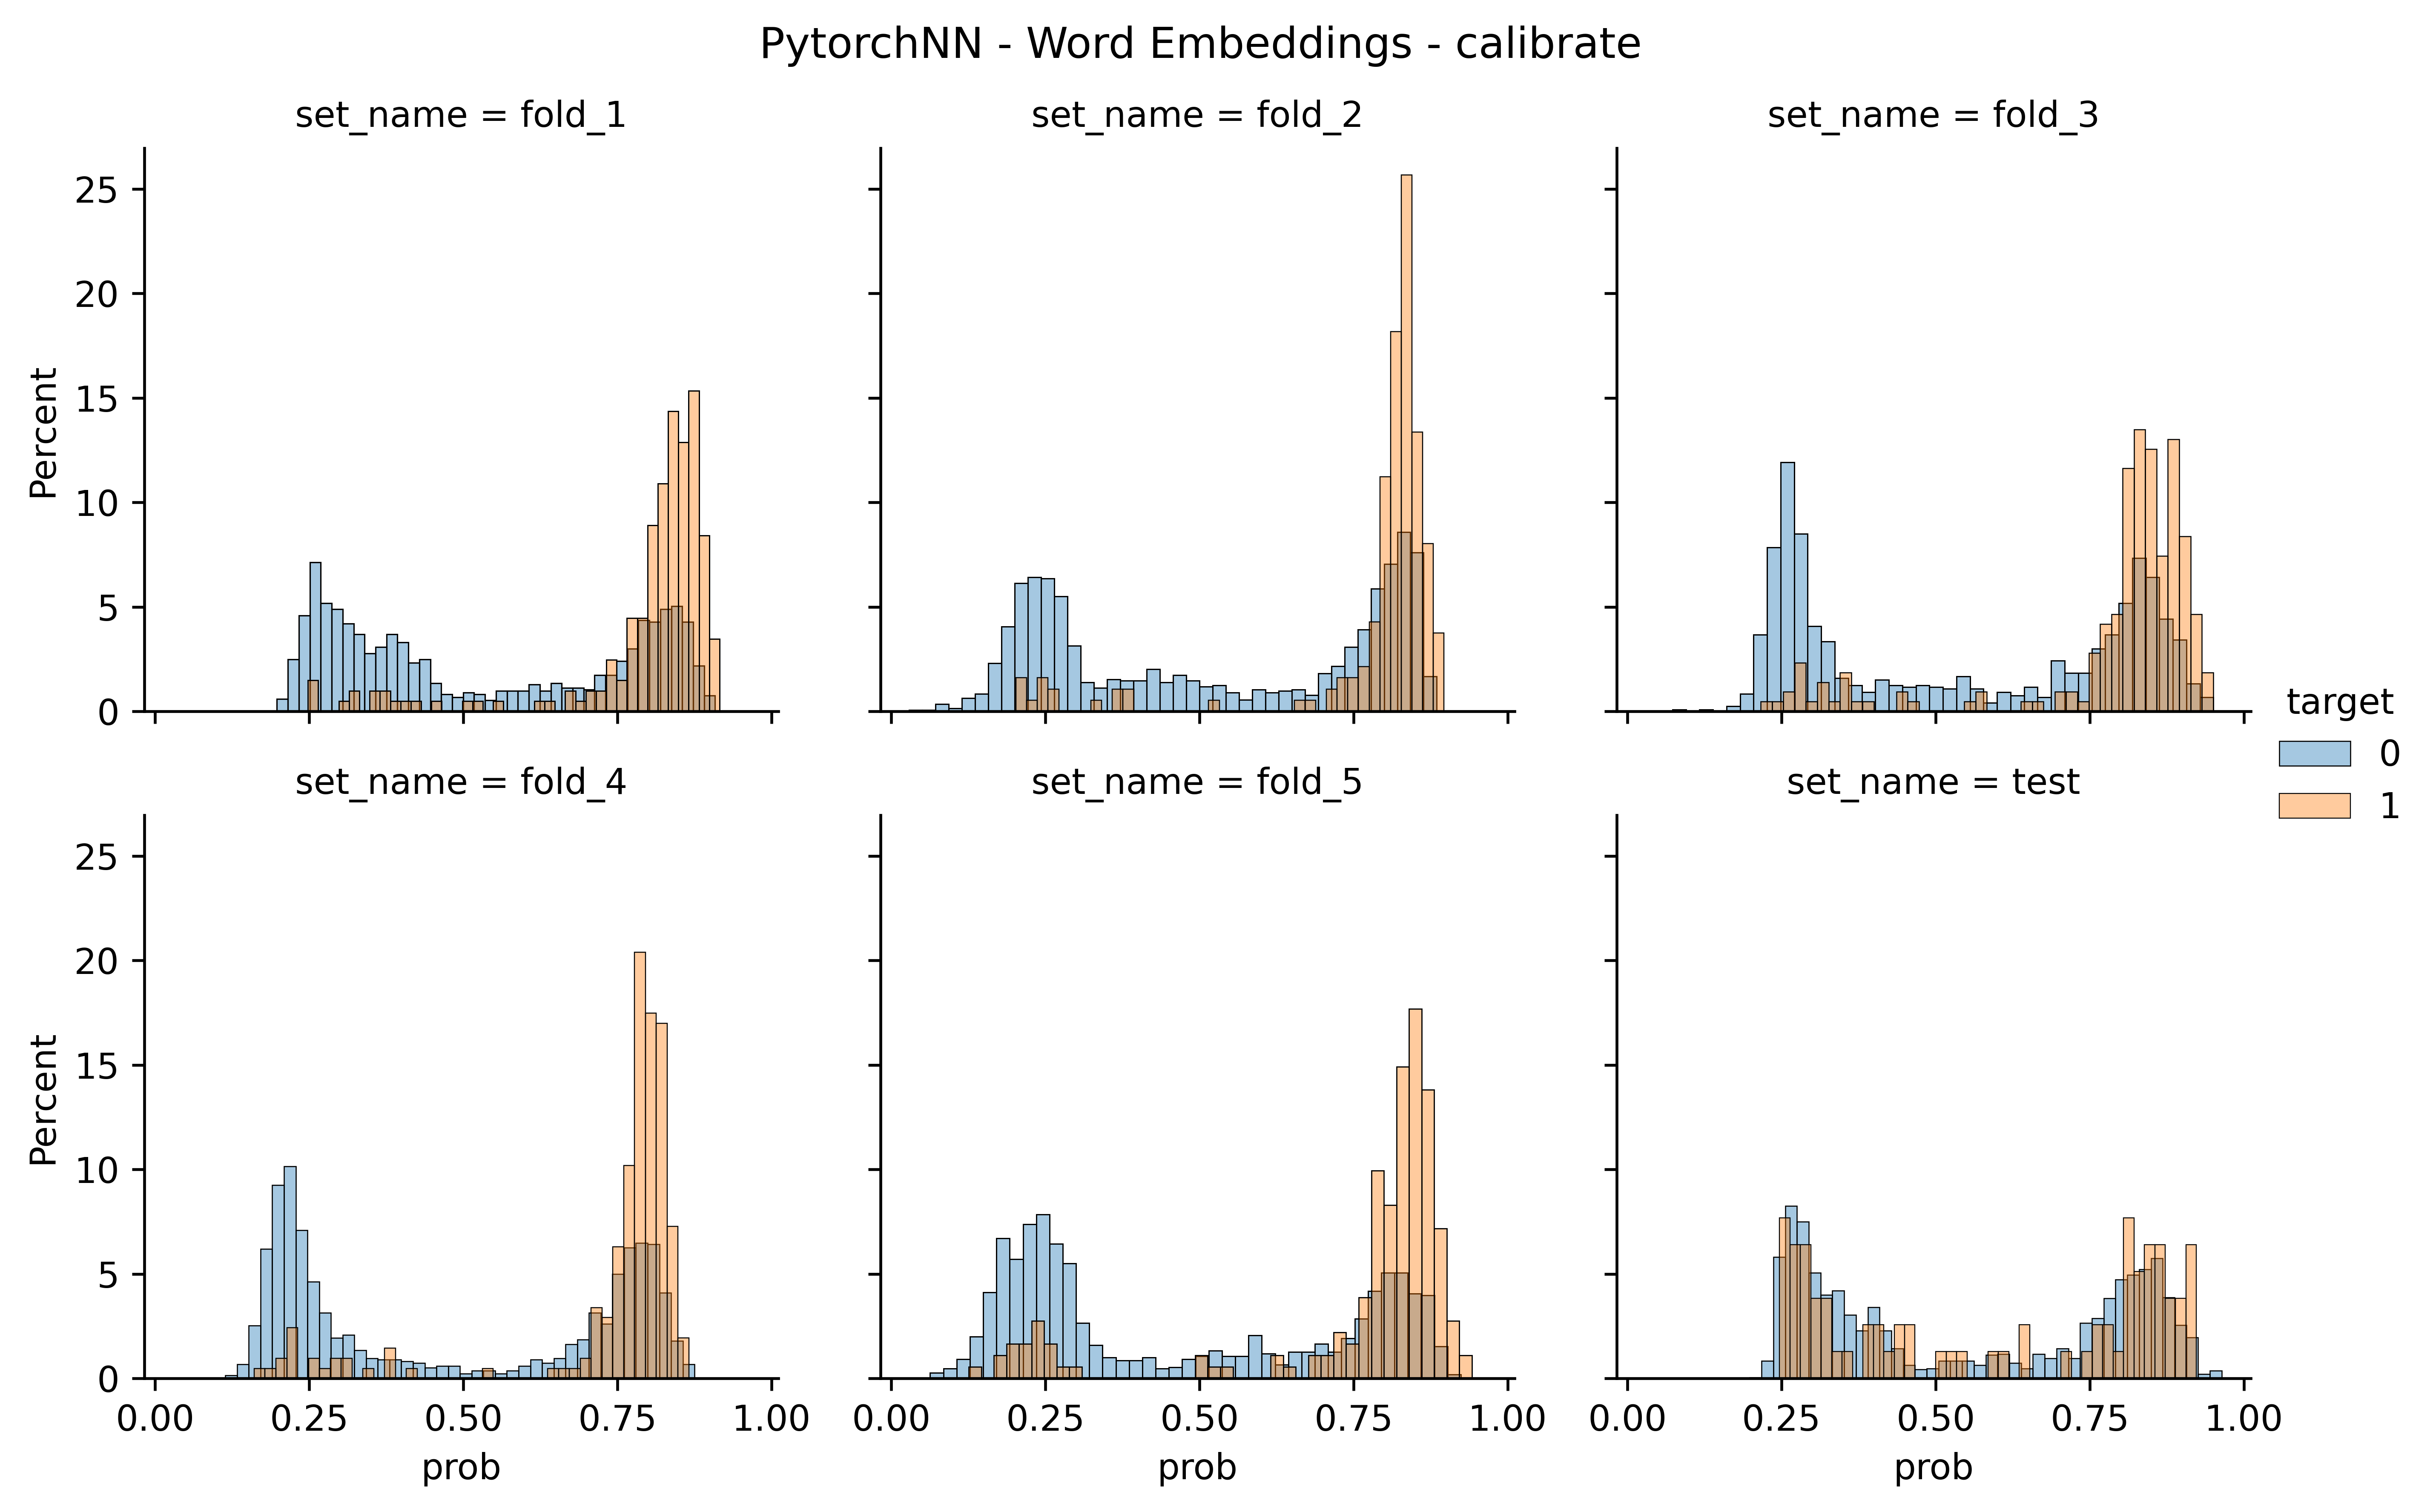
\includegraphics[width=\linewidth]{figures/results/word_embeddings/nn/calibrate/calibrate__distplot.png}
    \end{subfigure}
    \caption{Word embeddings calibrate}
\end{figure}

\begin{figure}
    \centering
    \begin{subfigure}[b]{0.83\textwidth}
    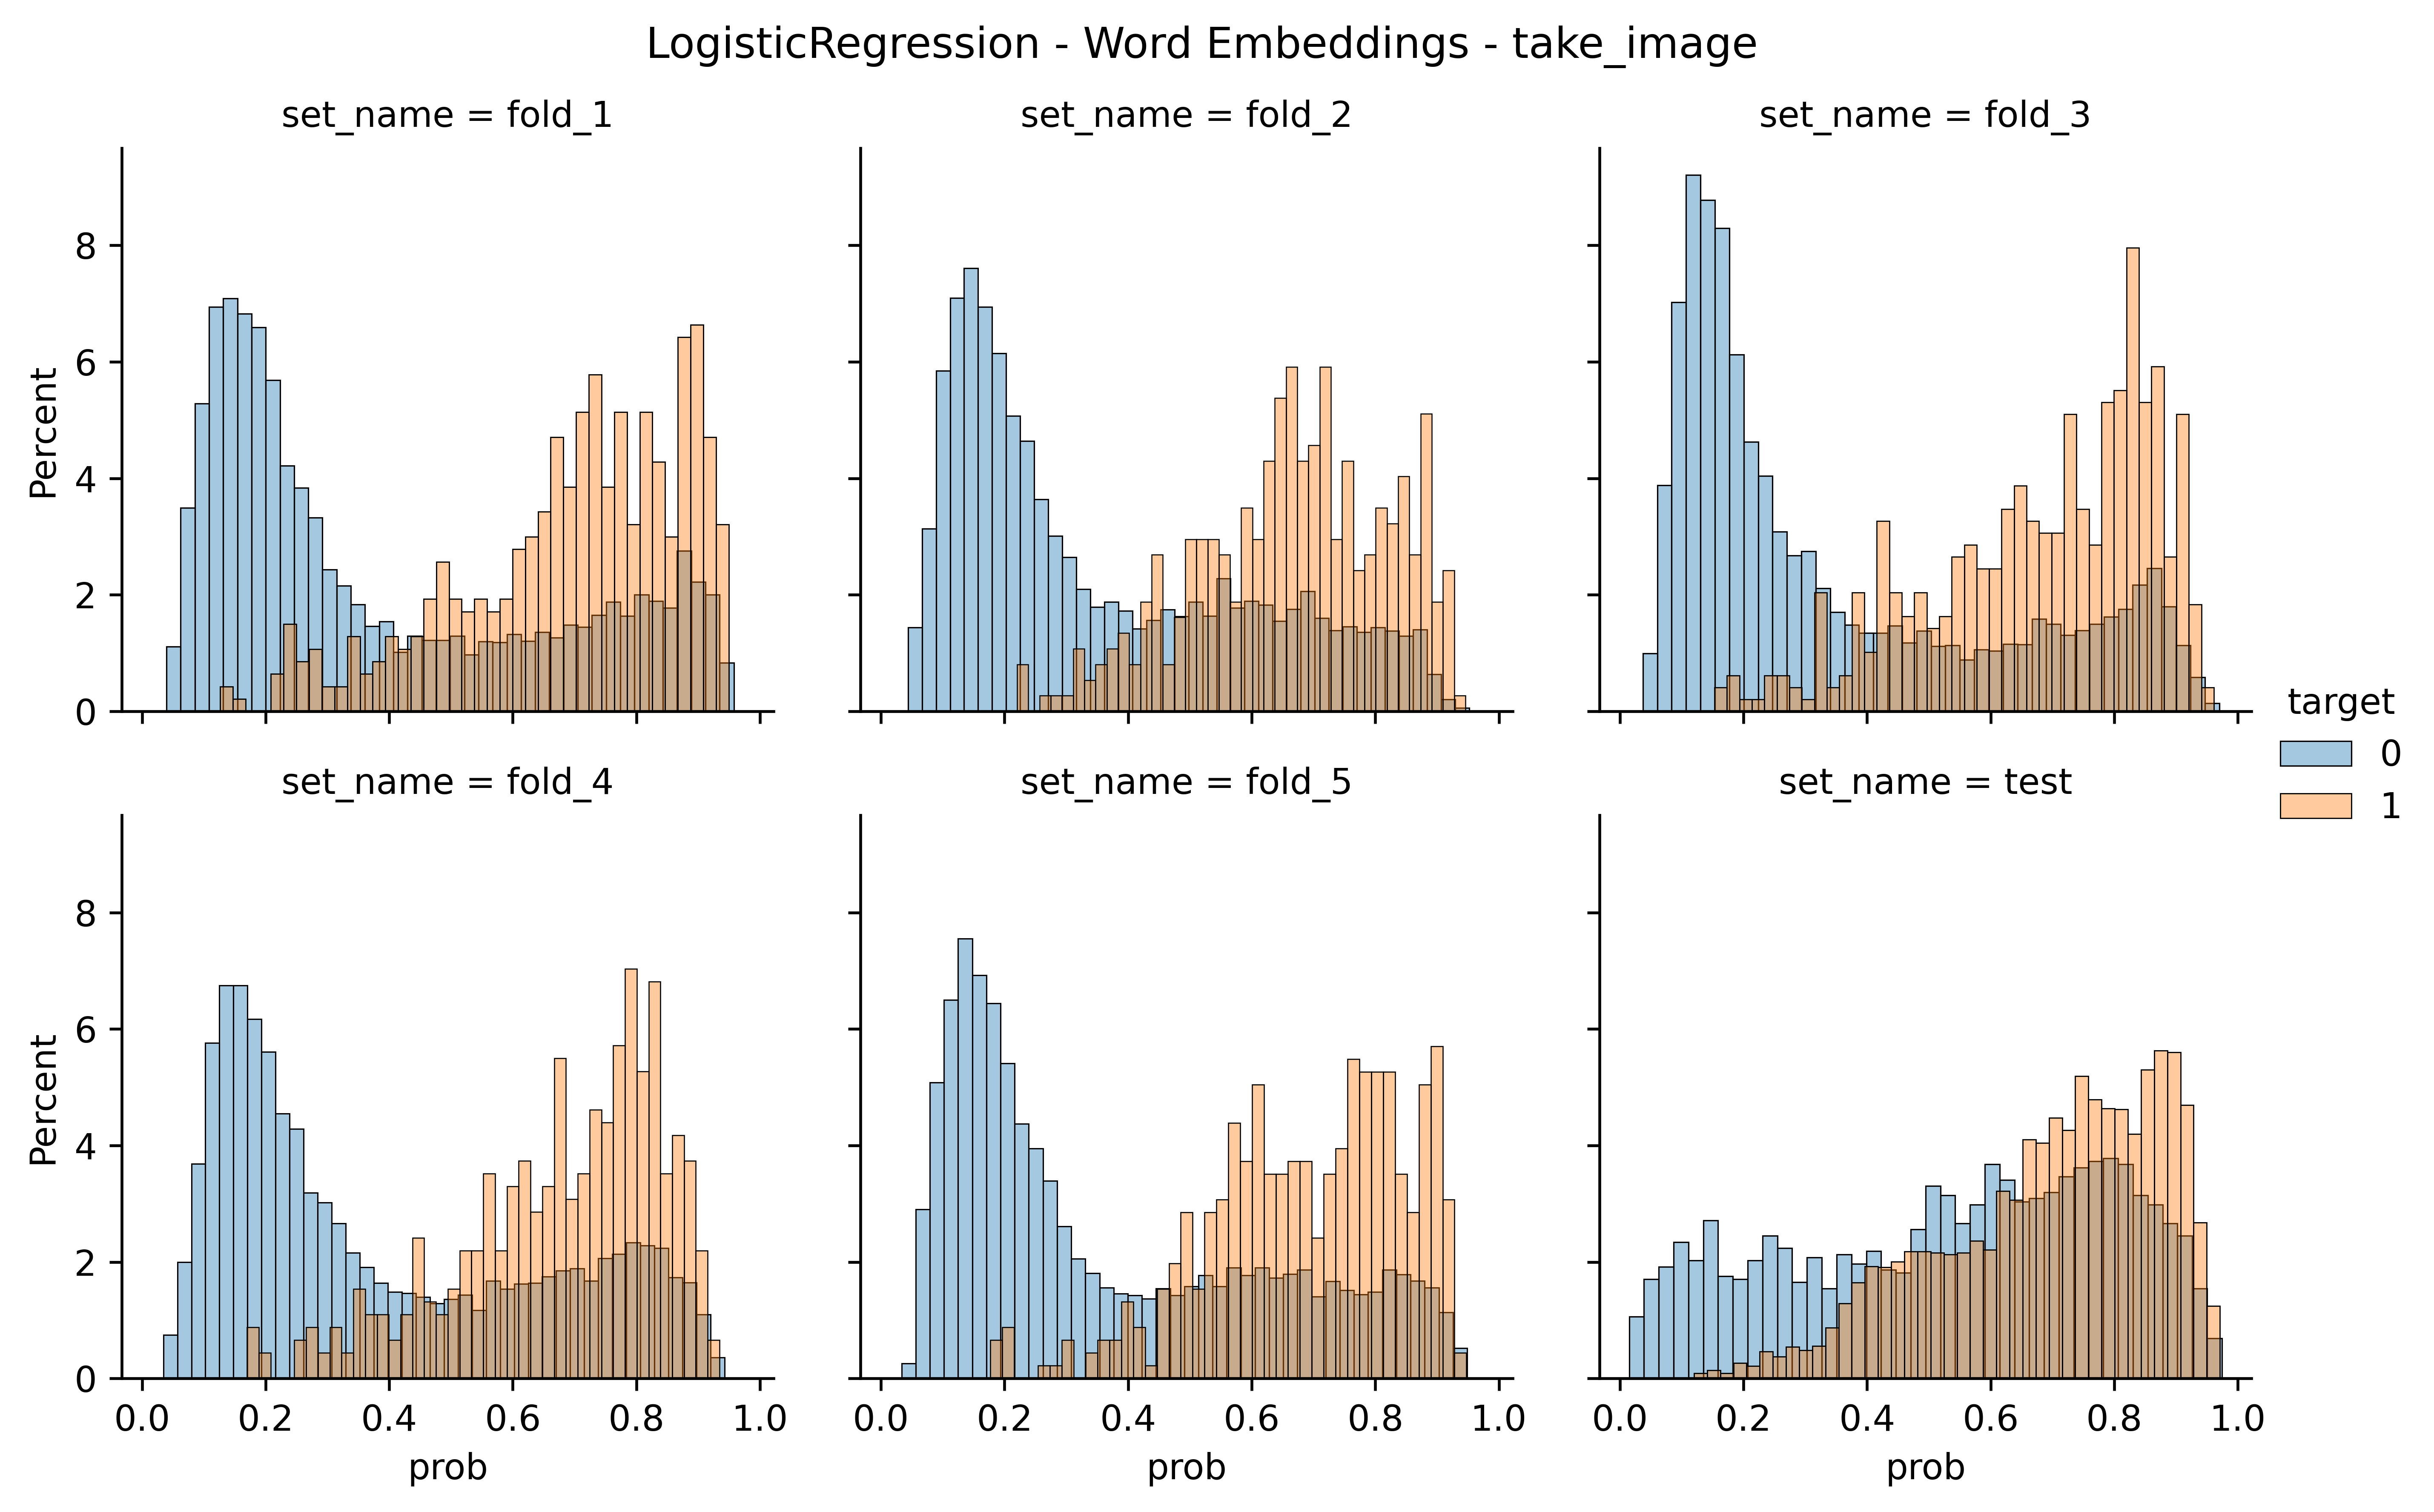
\includegraphics[width=\linewidth]{figures/results/word_embeddings/lgr/take_image/lgr__distplot.png}
    \end{subfigure}
    \hfill
    \centering
    \begin{subfigure}[b]{0.83\textwidth}
        \centering
        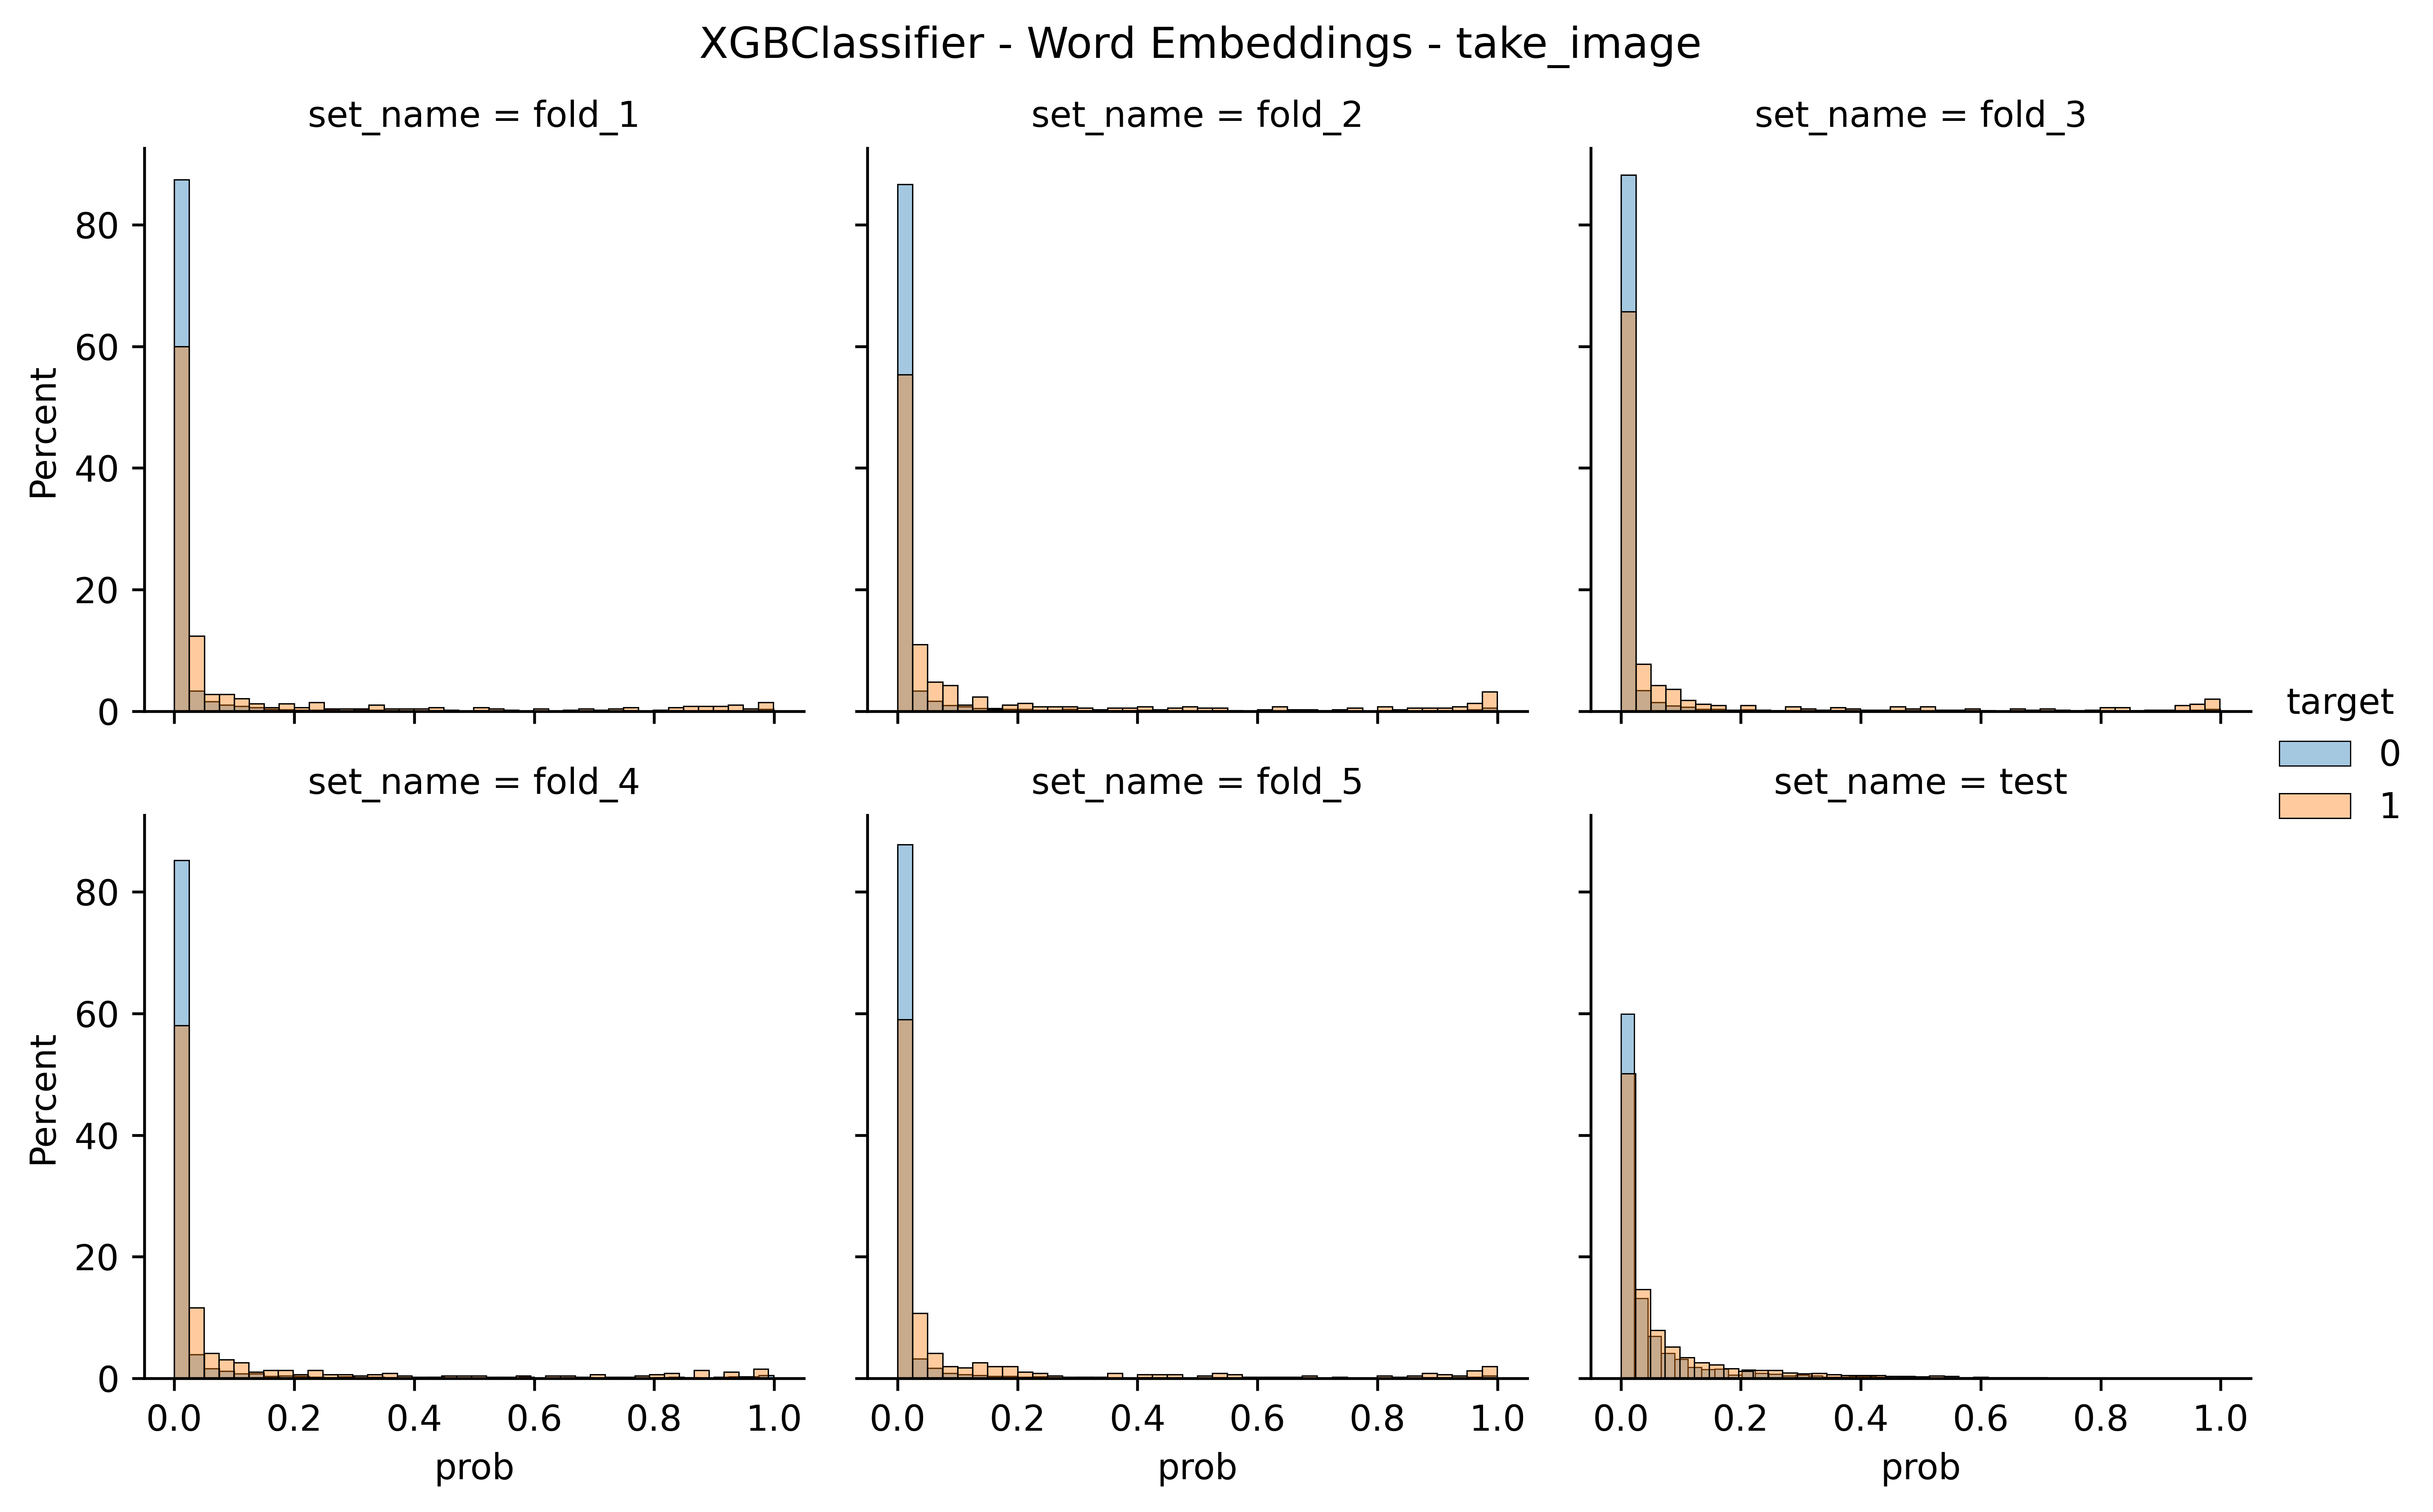
\includegraphics[width=\linewidth]{figures/results/word_embeddings/xgboost/take_image/take_image__distplot.png}
    \end{subfigure}
    \hfill
    \centering
    \begin{subfigure}[b]{0.83\textwidth}
        \centering
        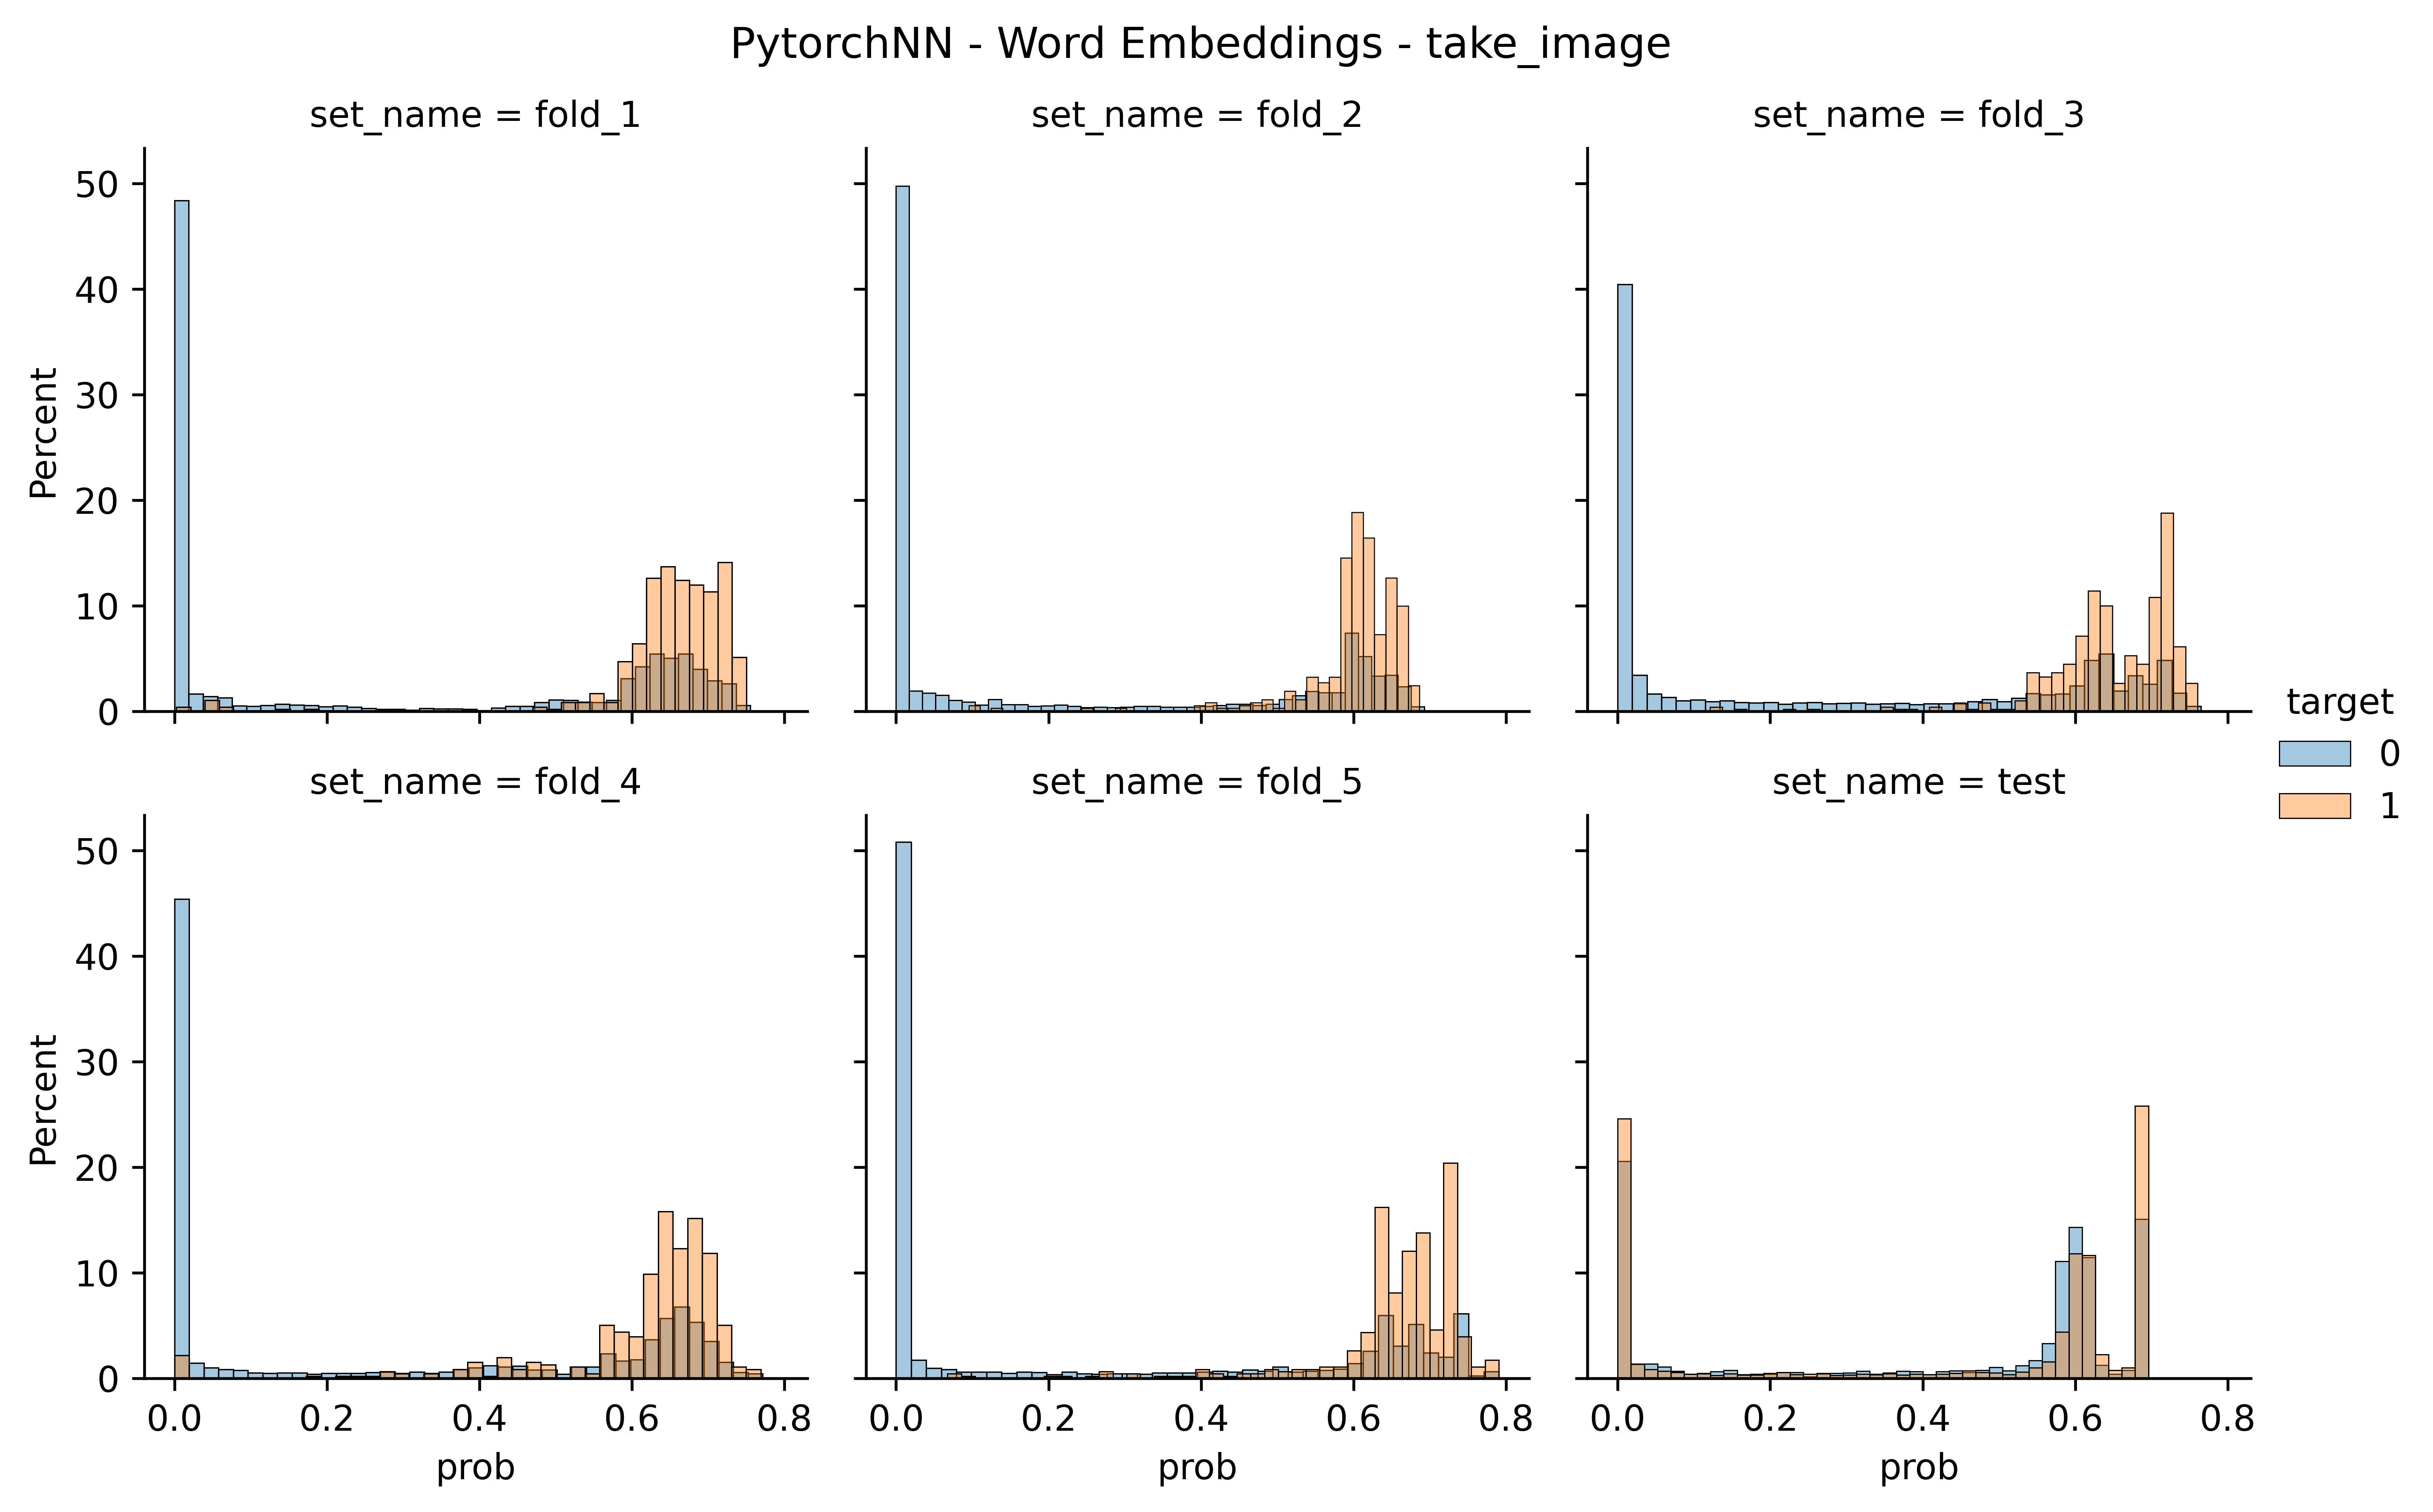
\includegraphics[width=\linewidth]{figures/results/word_embeddings/nn/take_image/take_image__distplot (1).png}
    \end{subfigure}
    \caption{Word embeddings take\_image}
\end{figure}

\begin{figure}
    \centering
    \begin{subfigure}[b]{0.83\textwidth}
    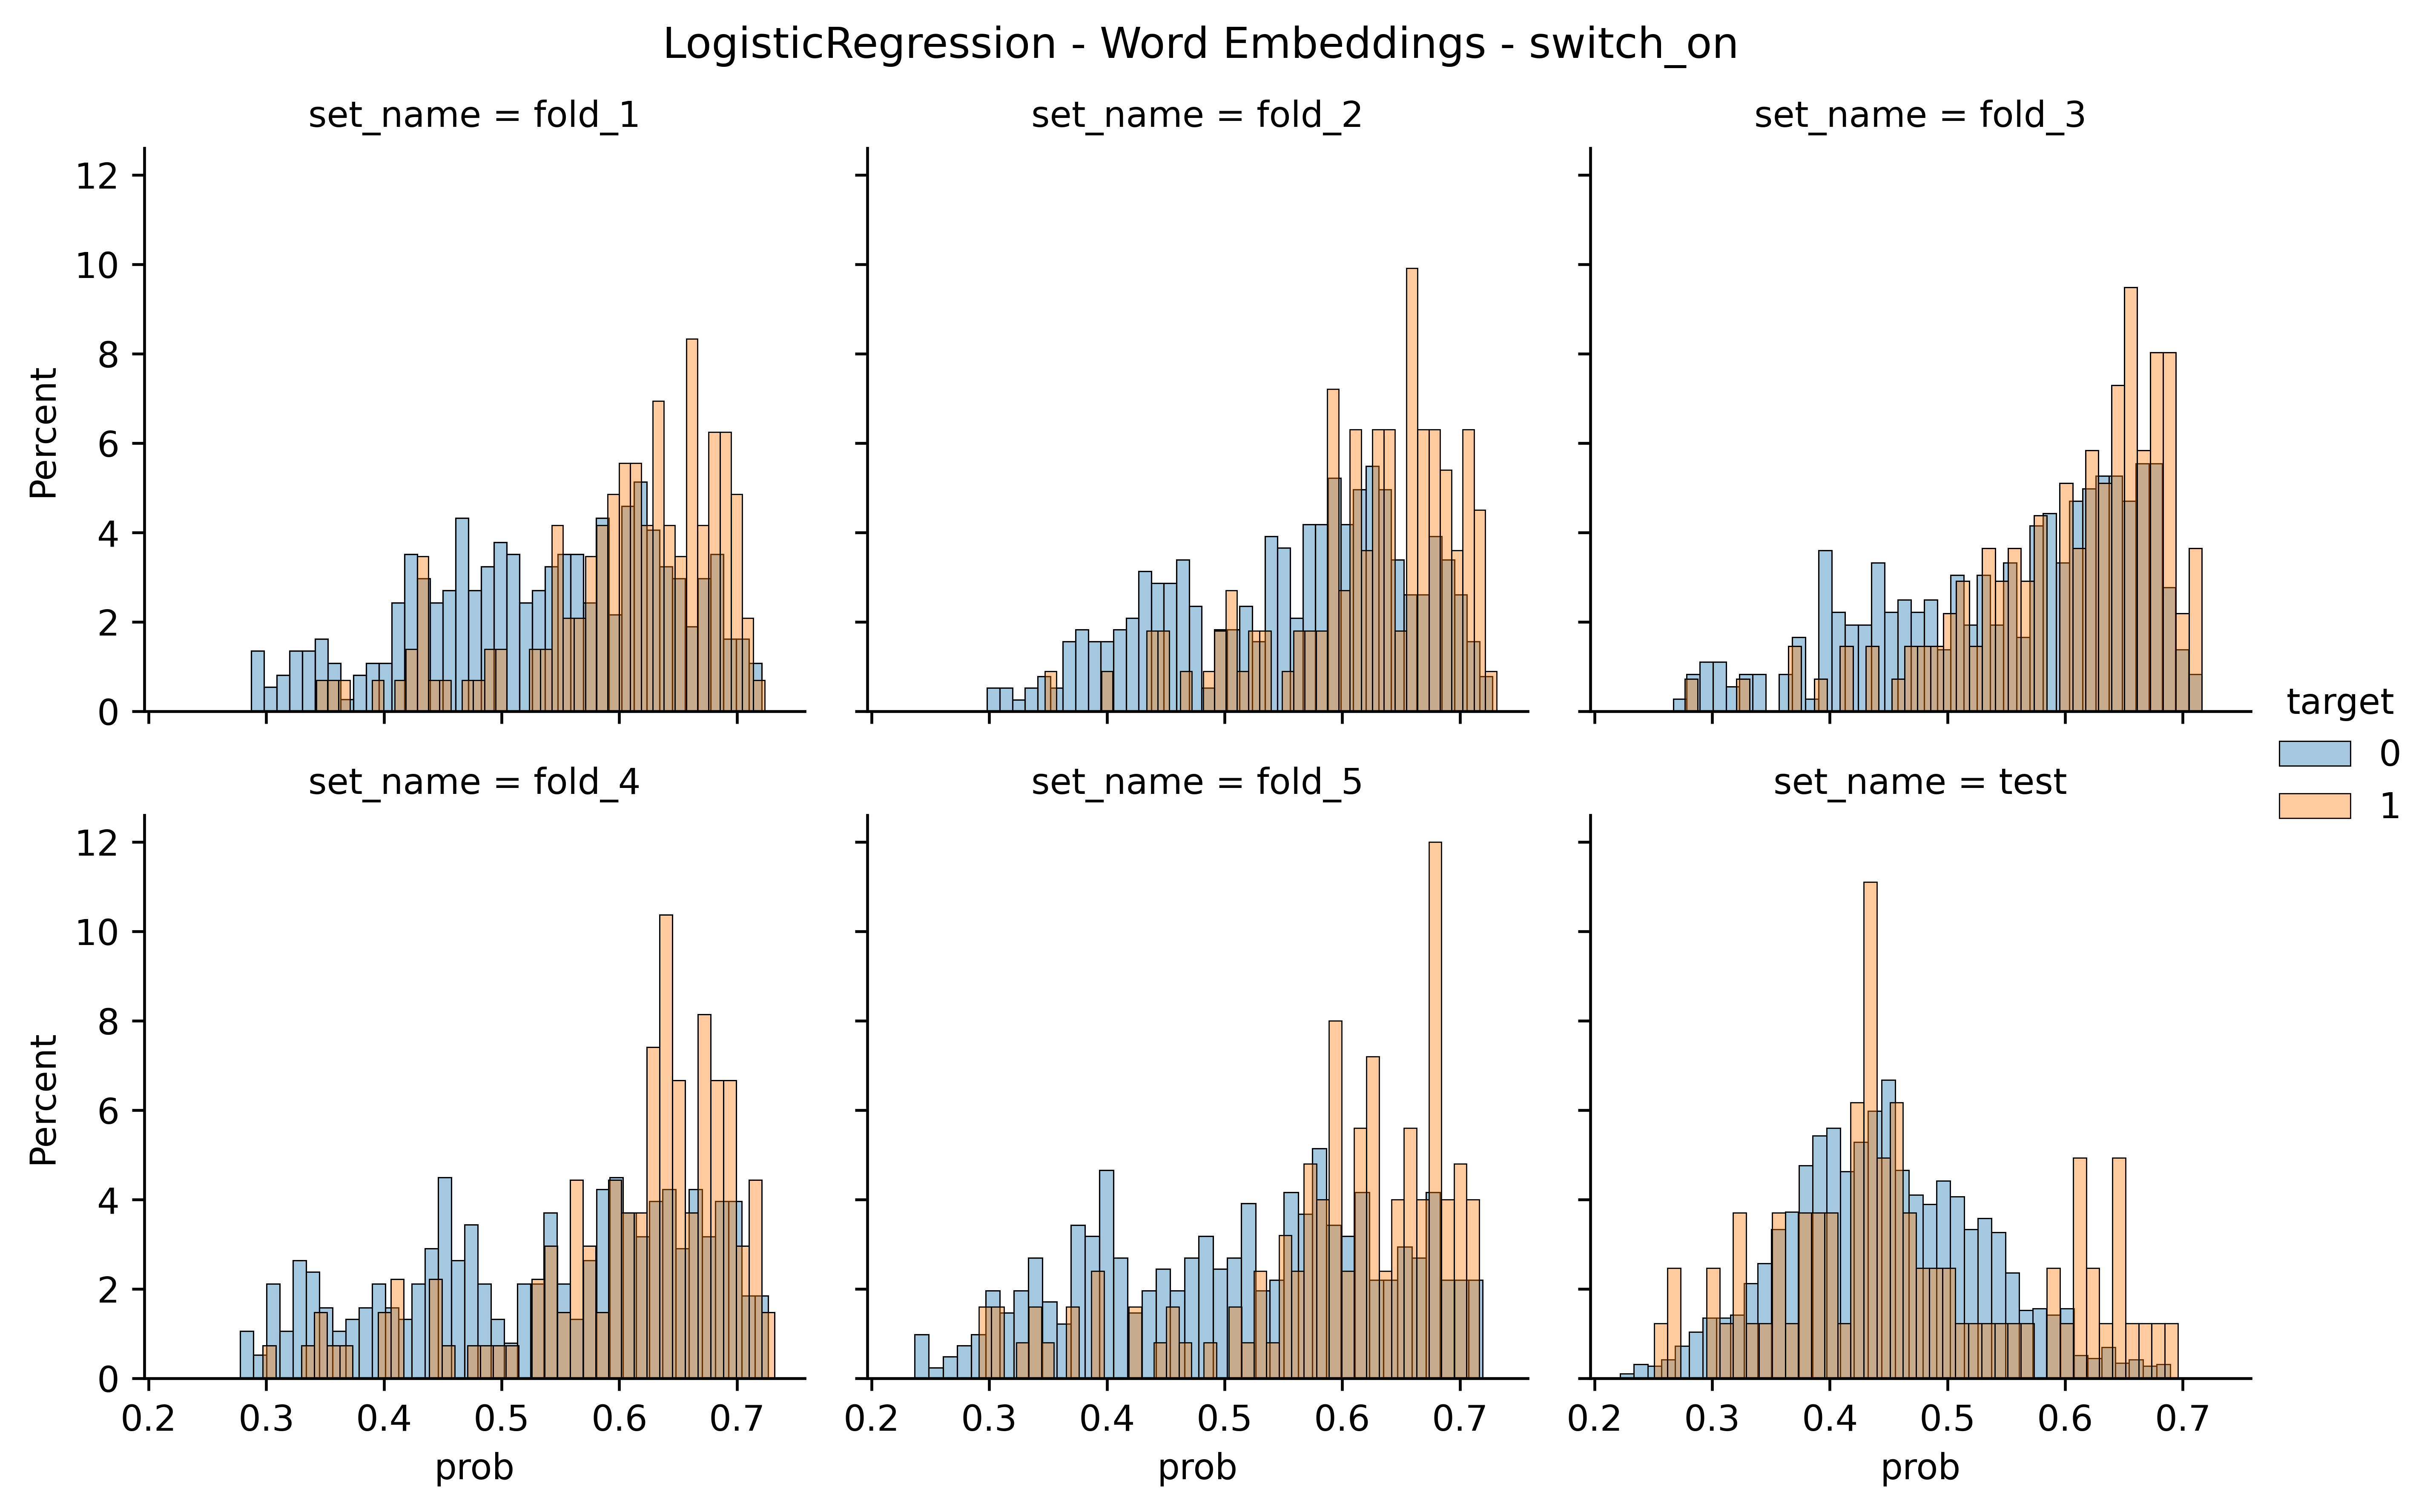
\includegraphics[width=\linewidth]{figures/results/word_embeddings/lgr/switch_on/switch_on__distplot.png}
    \end{subfigure}
    \hfill
    \centering
    \begin{subfigure}[b]{0.83\textwidth}
        \centering
        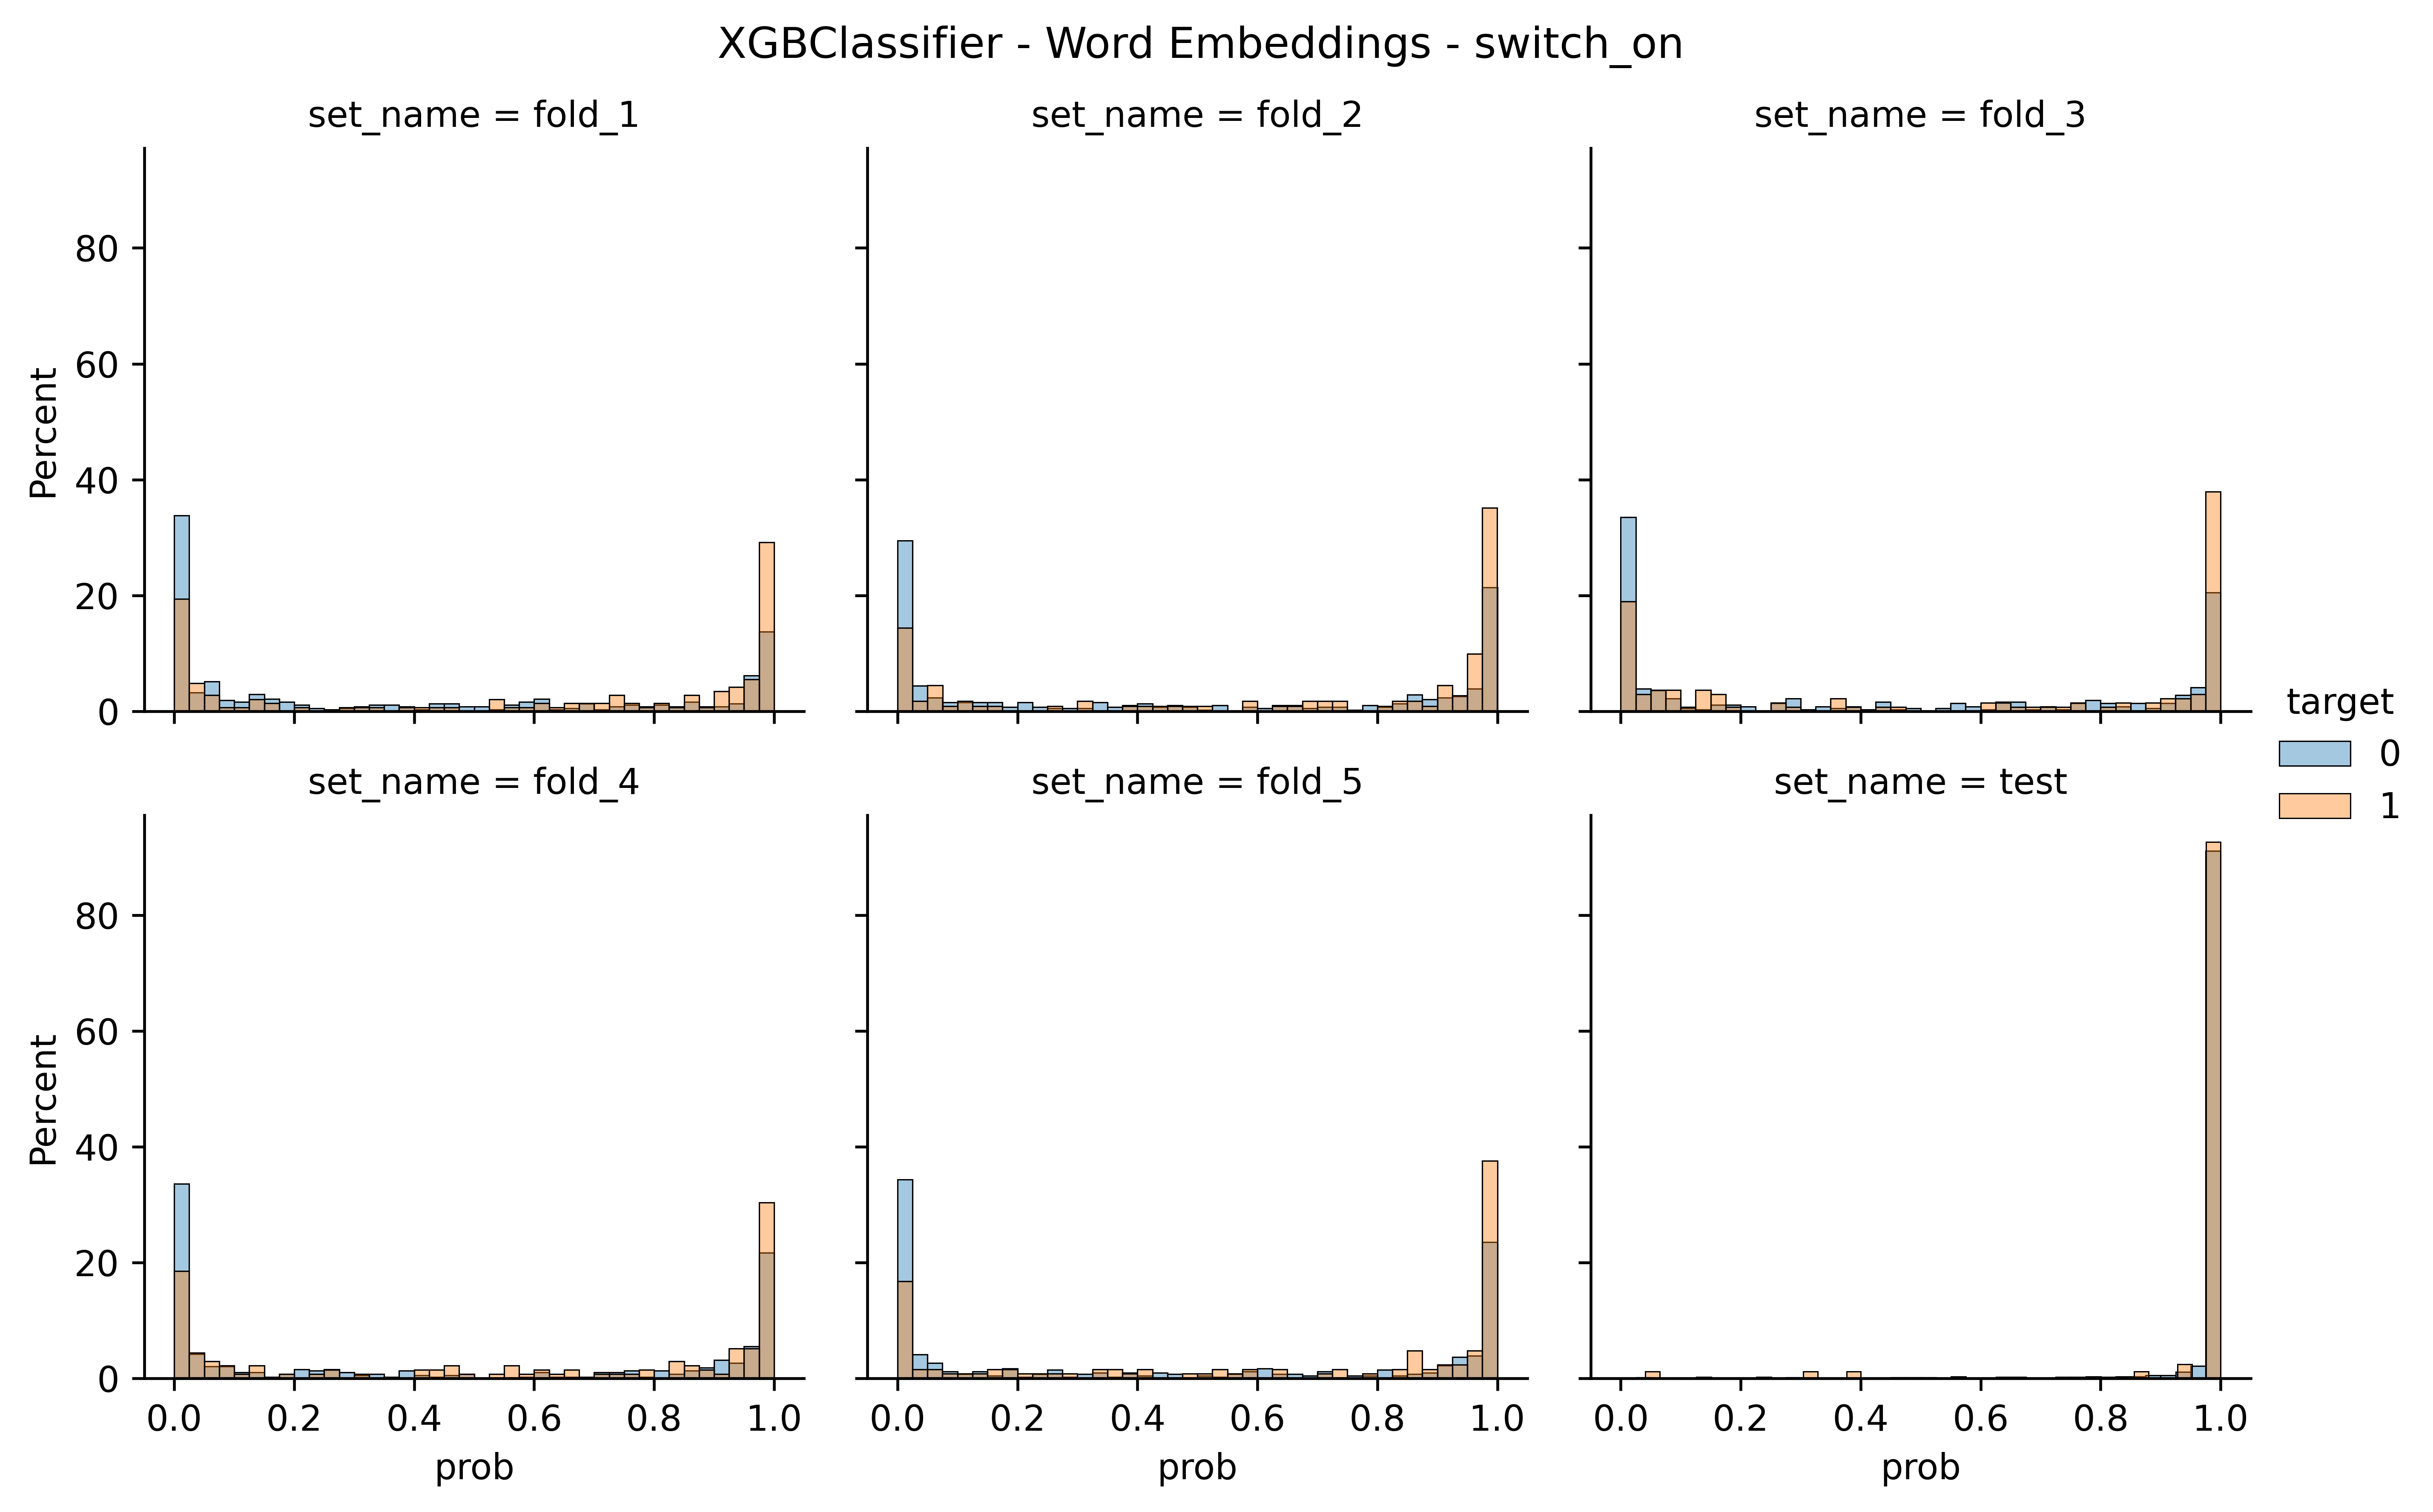
\includegraphics[width=\linewidth]{figures/results/word_embeddings/xgboost/switch_on/xgb__distplot.png}
    \end{subfigure}
    \hfill
    \centering
    \begin{subfigure}[b]{0.83\textwidth}
        \centering
        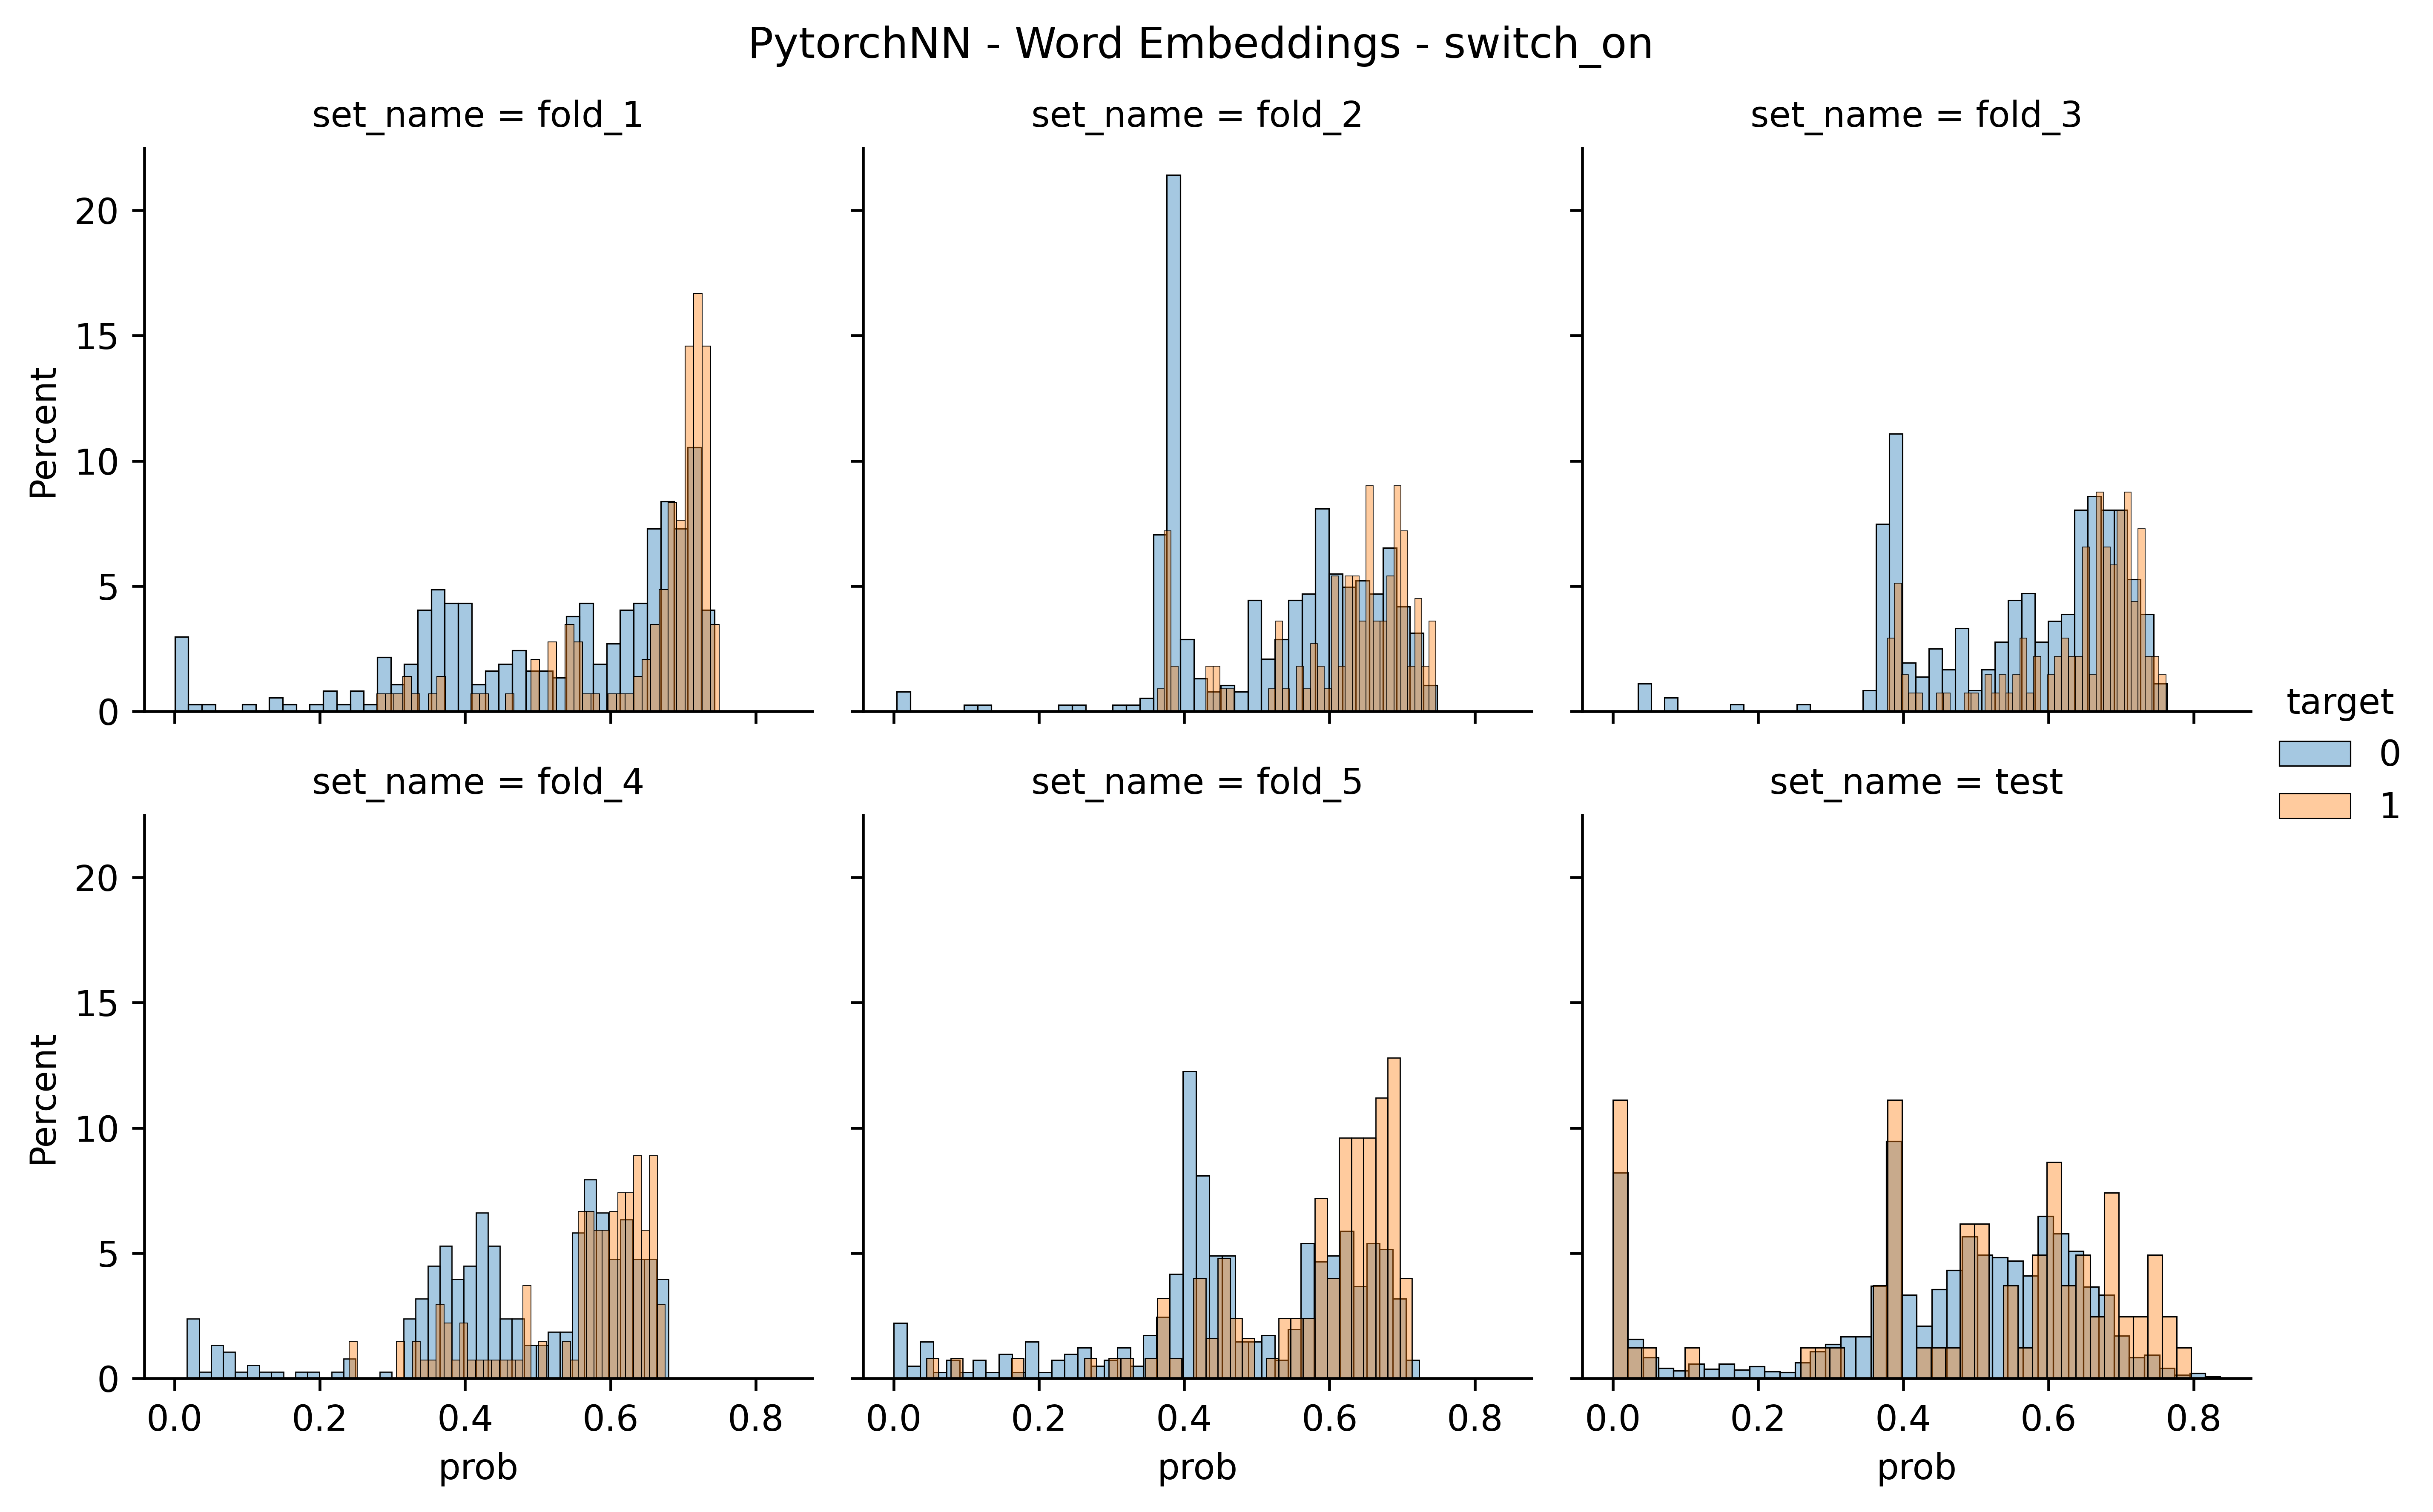
\includegraphics[width=\linewidth]{figures/results/word_embeddings/nn/switch_on/switch_on__distplot (1).png}
    \end{subfigure}
    \caption{Word embeddings switch\_on}
\end{figure}


\begin{figure}
    \begin{subfigure}[b]{\textwidth}
        \centering
        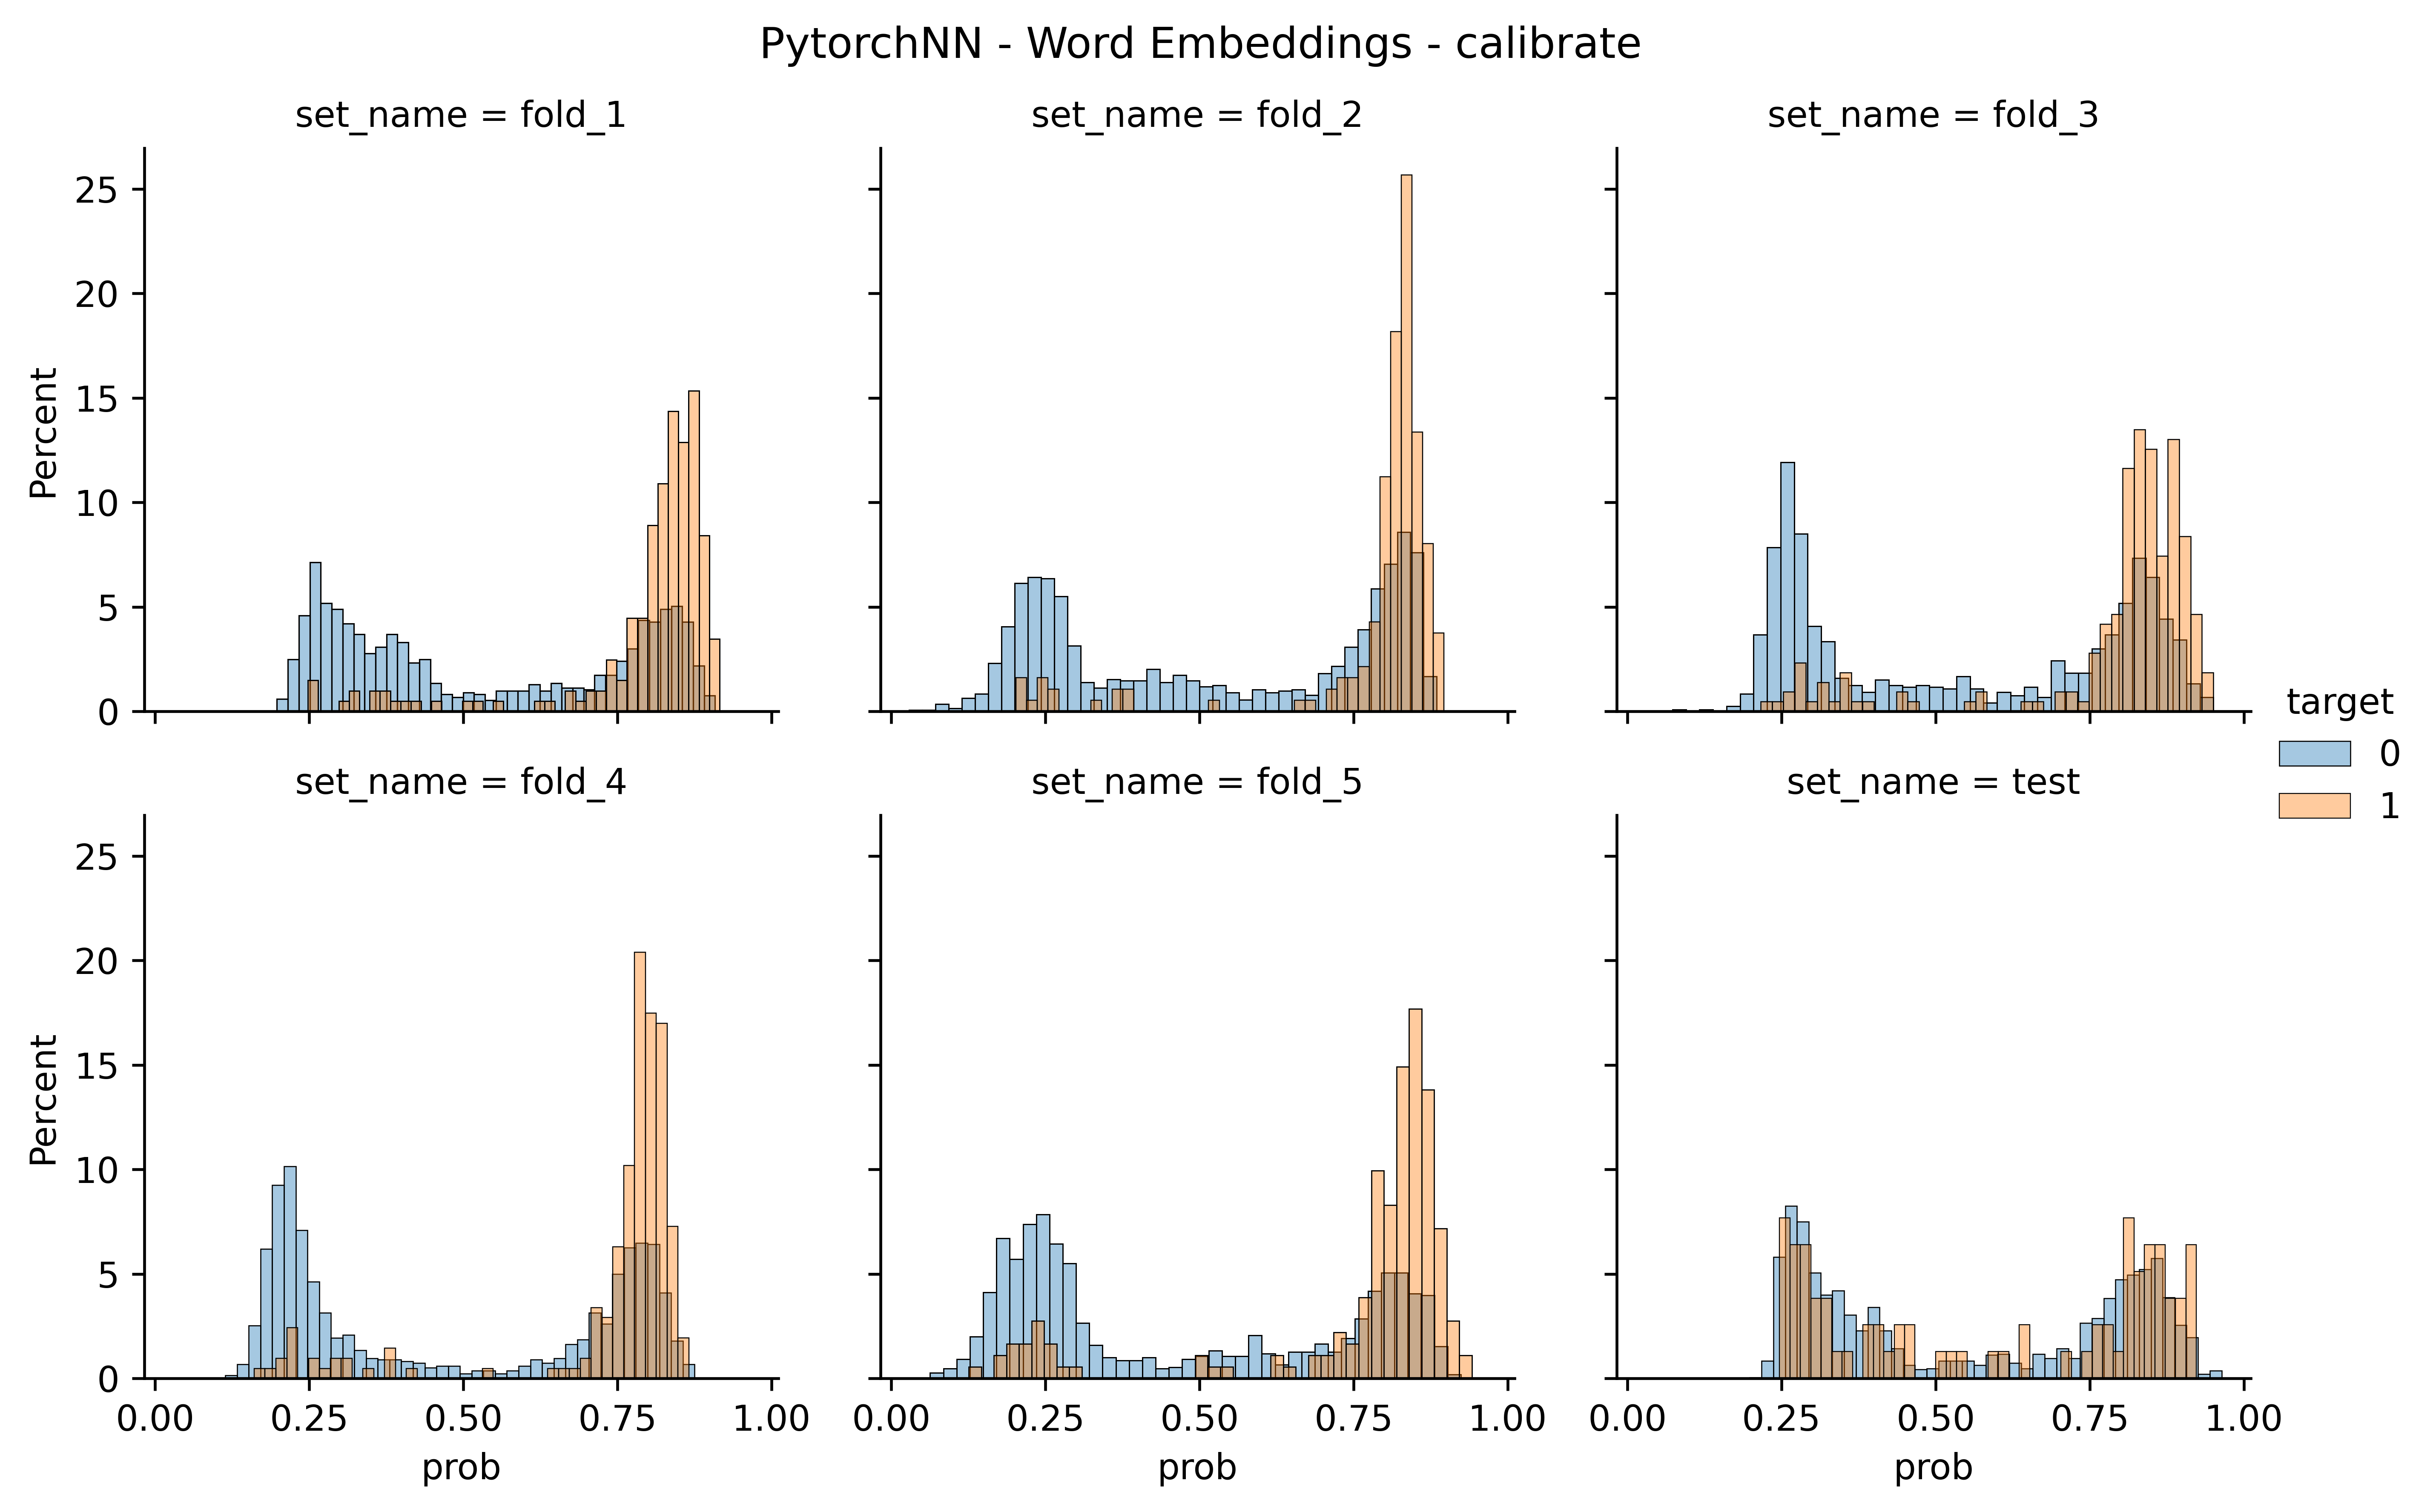
\includegraphics[width=\linewidth]{figures/results/word_embeddings/nn/calibrate/calibrate__distplot.png}
        \caption{Distribución de predicciones en validación cruzada y el conjunto de test.}
        \label{fig:my_label}
    \end{subfigure}
    \hfill
    \begin{subfigure}[b]{\textwidth}
    \minipage{0.32\textwidth}
      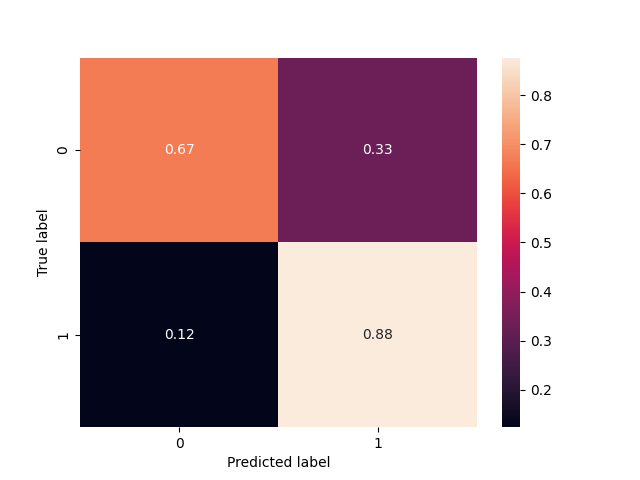
\includegraphics[width=\linewidth]{figures/results/word_embeddings/nn/calibrate/calibrate_set_1_confusion_matrix_percent.png}
    \endminipage\hfill
    \minipage{0.32\textwidth}
      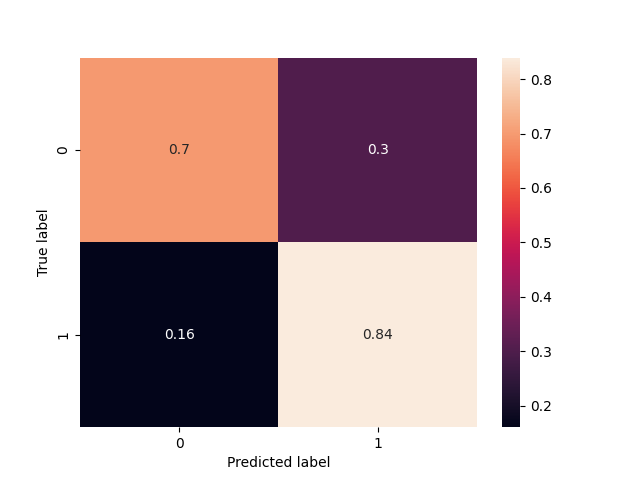
\includegraphics[width=\linewidth]{figures/results/word_embeddings/nn/calibrate/calibrate_set_2_confusion_matrix_percent.png}
    \endminipage\hfill \minipage{0.32\textwidth}%
      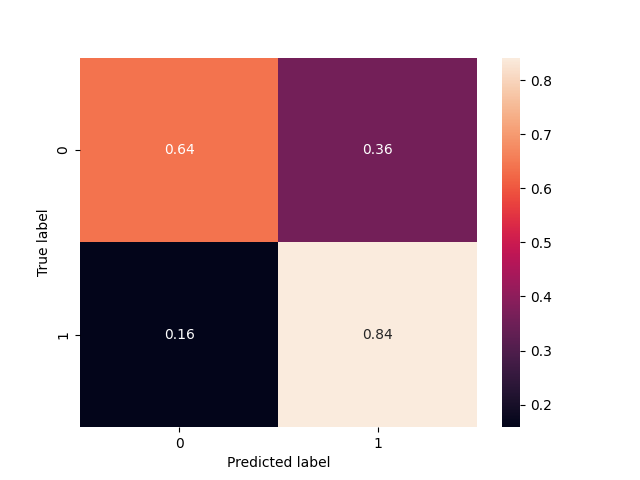
\includegraphics[width=\linewidth]{figures/results/word_embeddings/nn/calibrate/calibrate+_set_3_confusion_matrix_percent.png}
    \endminipage
    
    \medskip
    
    \minipage{0.32\textwidth}
      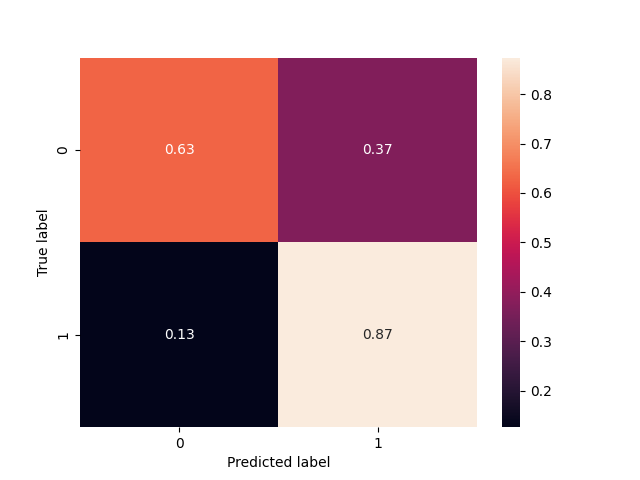
\includegraphics[width=\linewidth]{figures/results/word_embeddings/nn/calibrate/calibrate_set_4_confusion_matrix_percent.png}
    \endminipage\hfill
    \minipage{0.32\textwidth}
    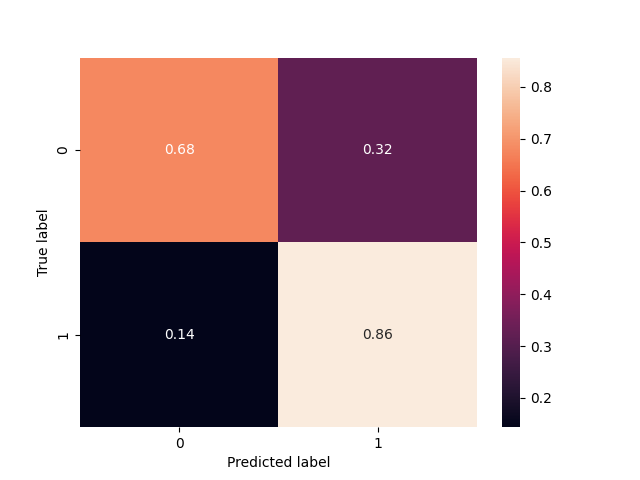
\includegraphics[width=\linewidth]{figures/results/word_embeddings/nn/calibrate/calibrate_set_5_confusion_matrix_percent.png}
    \endminipage\hfill \minipage{0.32\textwidth}%
    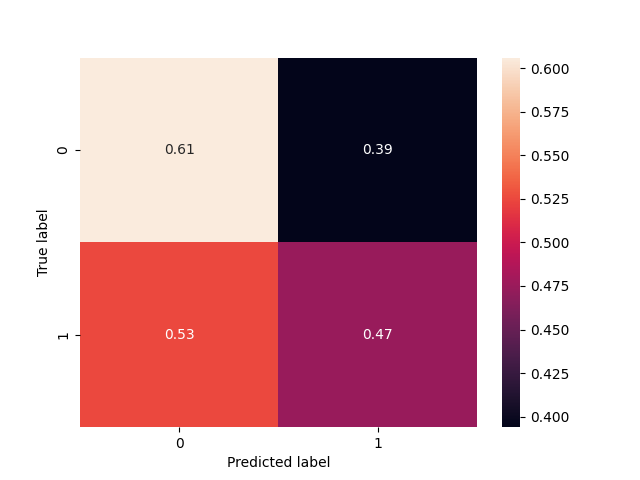
\includegraphics[width=\linewidth]{figures/results/word_embeddings/nn/calibrate/calibrate_set_6_confusion_matrix_percent.png}
    \endminipage
    \caption{Matrices de confusión en validación cruzada y el conjunto de test}
    \end{subfigure}
    \caption{Resultados del modelo de redes neuronales con codificación por word embeddings y esquema de acción calibrate.}
\end{figure}

\begin{table}[h!]
\centering
\scalebox{0.9}{
 \begin{tabular}{|c || c | c | c | c | c | c |} 
 \hline
  Esquemas & Precisión & Recall & $H_{1.5}$ & $F_{1.5}$ & Umbral de decisión &
  Modelo \\
 \hline
 take\_image & 0.8088 & 0.997 & 0.4351 & 0.997 & 0.61 & LGR \\
 calibrate & 0.0467 & 0.4743 & 0.5083 & 0.1242 & 0.728 & NN\\
 switch\_on  & 0.0405 & 0.4567 & 0.5106 & 0.1097 & 0.576 & NN\\
 switch\_off & 0.0476 & 0.1818 & 0.2422 & 0.0876 & 0.034 & NN \\
 turn\_to  & - & - & - & - & - & -\\[1ex]
 \hline
 \end{tabular}}
 \caption{Resultados por esquema de acción del mejor modelo con codificación por word embeddings.}
 \label{results:ad-hoc-calibrate}
\end{table}


\section{Modelos predictivos ad-hoc}
\label{exp:wb}

\subsection{Configuración del experimento}

Como contraparte del experimento anterior, usaremos la codificación por word
embeddings, bajo el mismo conjunto de entrenamientos y construcción de ventanas,
con la salvedad de ser codificados a partir del modelo de lenguaje de FastText,
entrenado con oraciones provenientes de planes relajados. El modelo de lenguaje
es un modelo Skipgram entrenado por $100$ épocas, un tamaño de ventana de
contexto de $3$ palabras, y un vector de salida de dimensión $30$. Se hicieron
pruebas sobre otras configuraciones de parámetros pero el comportamiento que
buscábamos que el modelo de lenguaje aprendiese ya era obtenido bajo esta
configuración.

Los clasificadores y grillas de búsqueda de parámetros utilizadas fueron las
mismos que los modelo predictivos ad-hoc.

\subsection{Resultados}

\begin{figure}
    \centering
    \begin{subfigure}[b]{0.83\textwidth}
    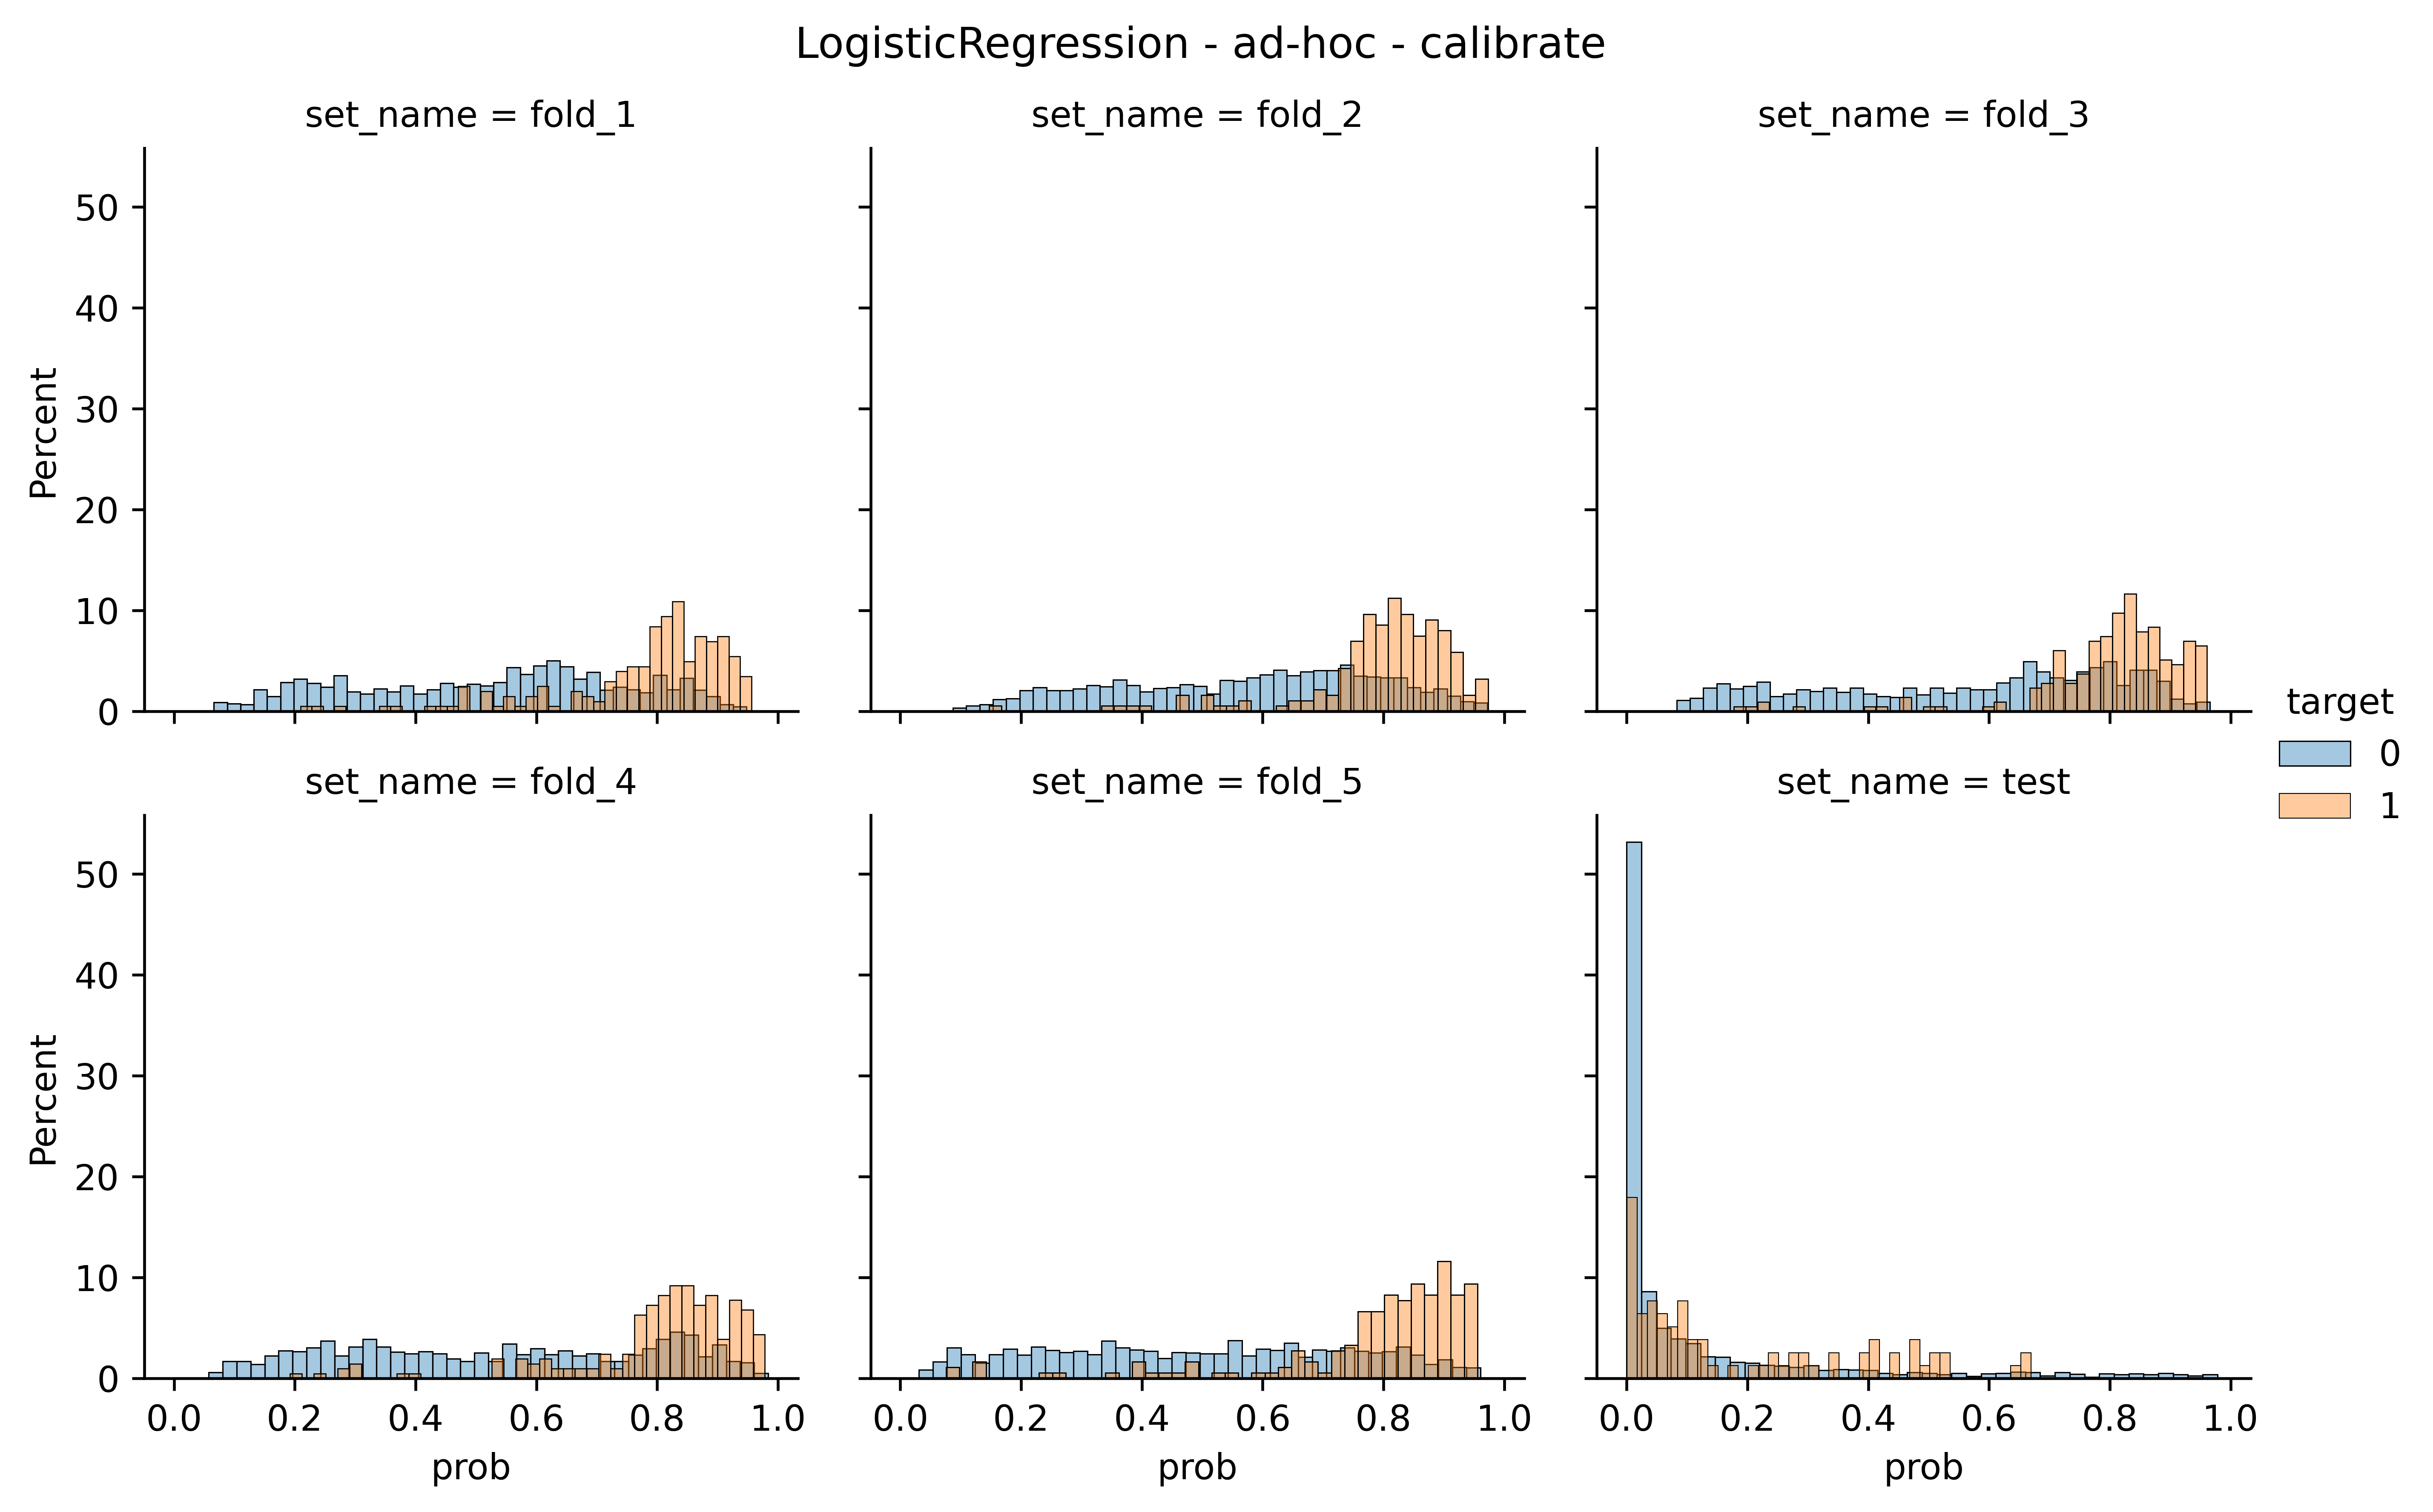
\includegraphics[width=\linewidth]{figures/results/ad-hoc/lgr/calibrate/calibrate__distplot.png}
    \end{subfigure}
    \hfill
    \centering
    \begin{subfigure}[b]{0.83\textwidth}
        \centering
        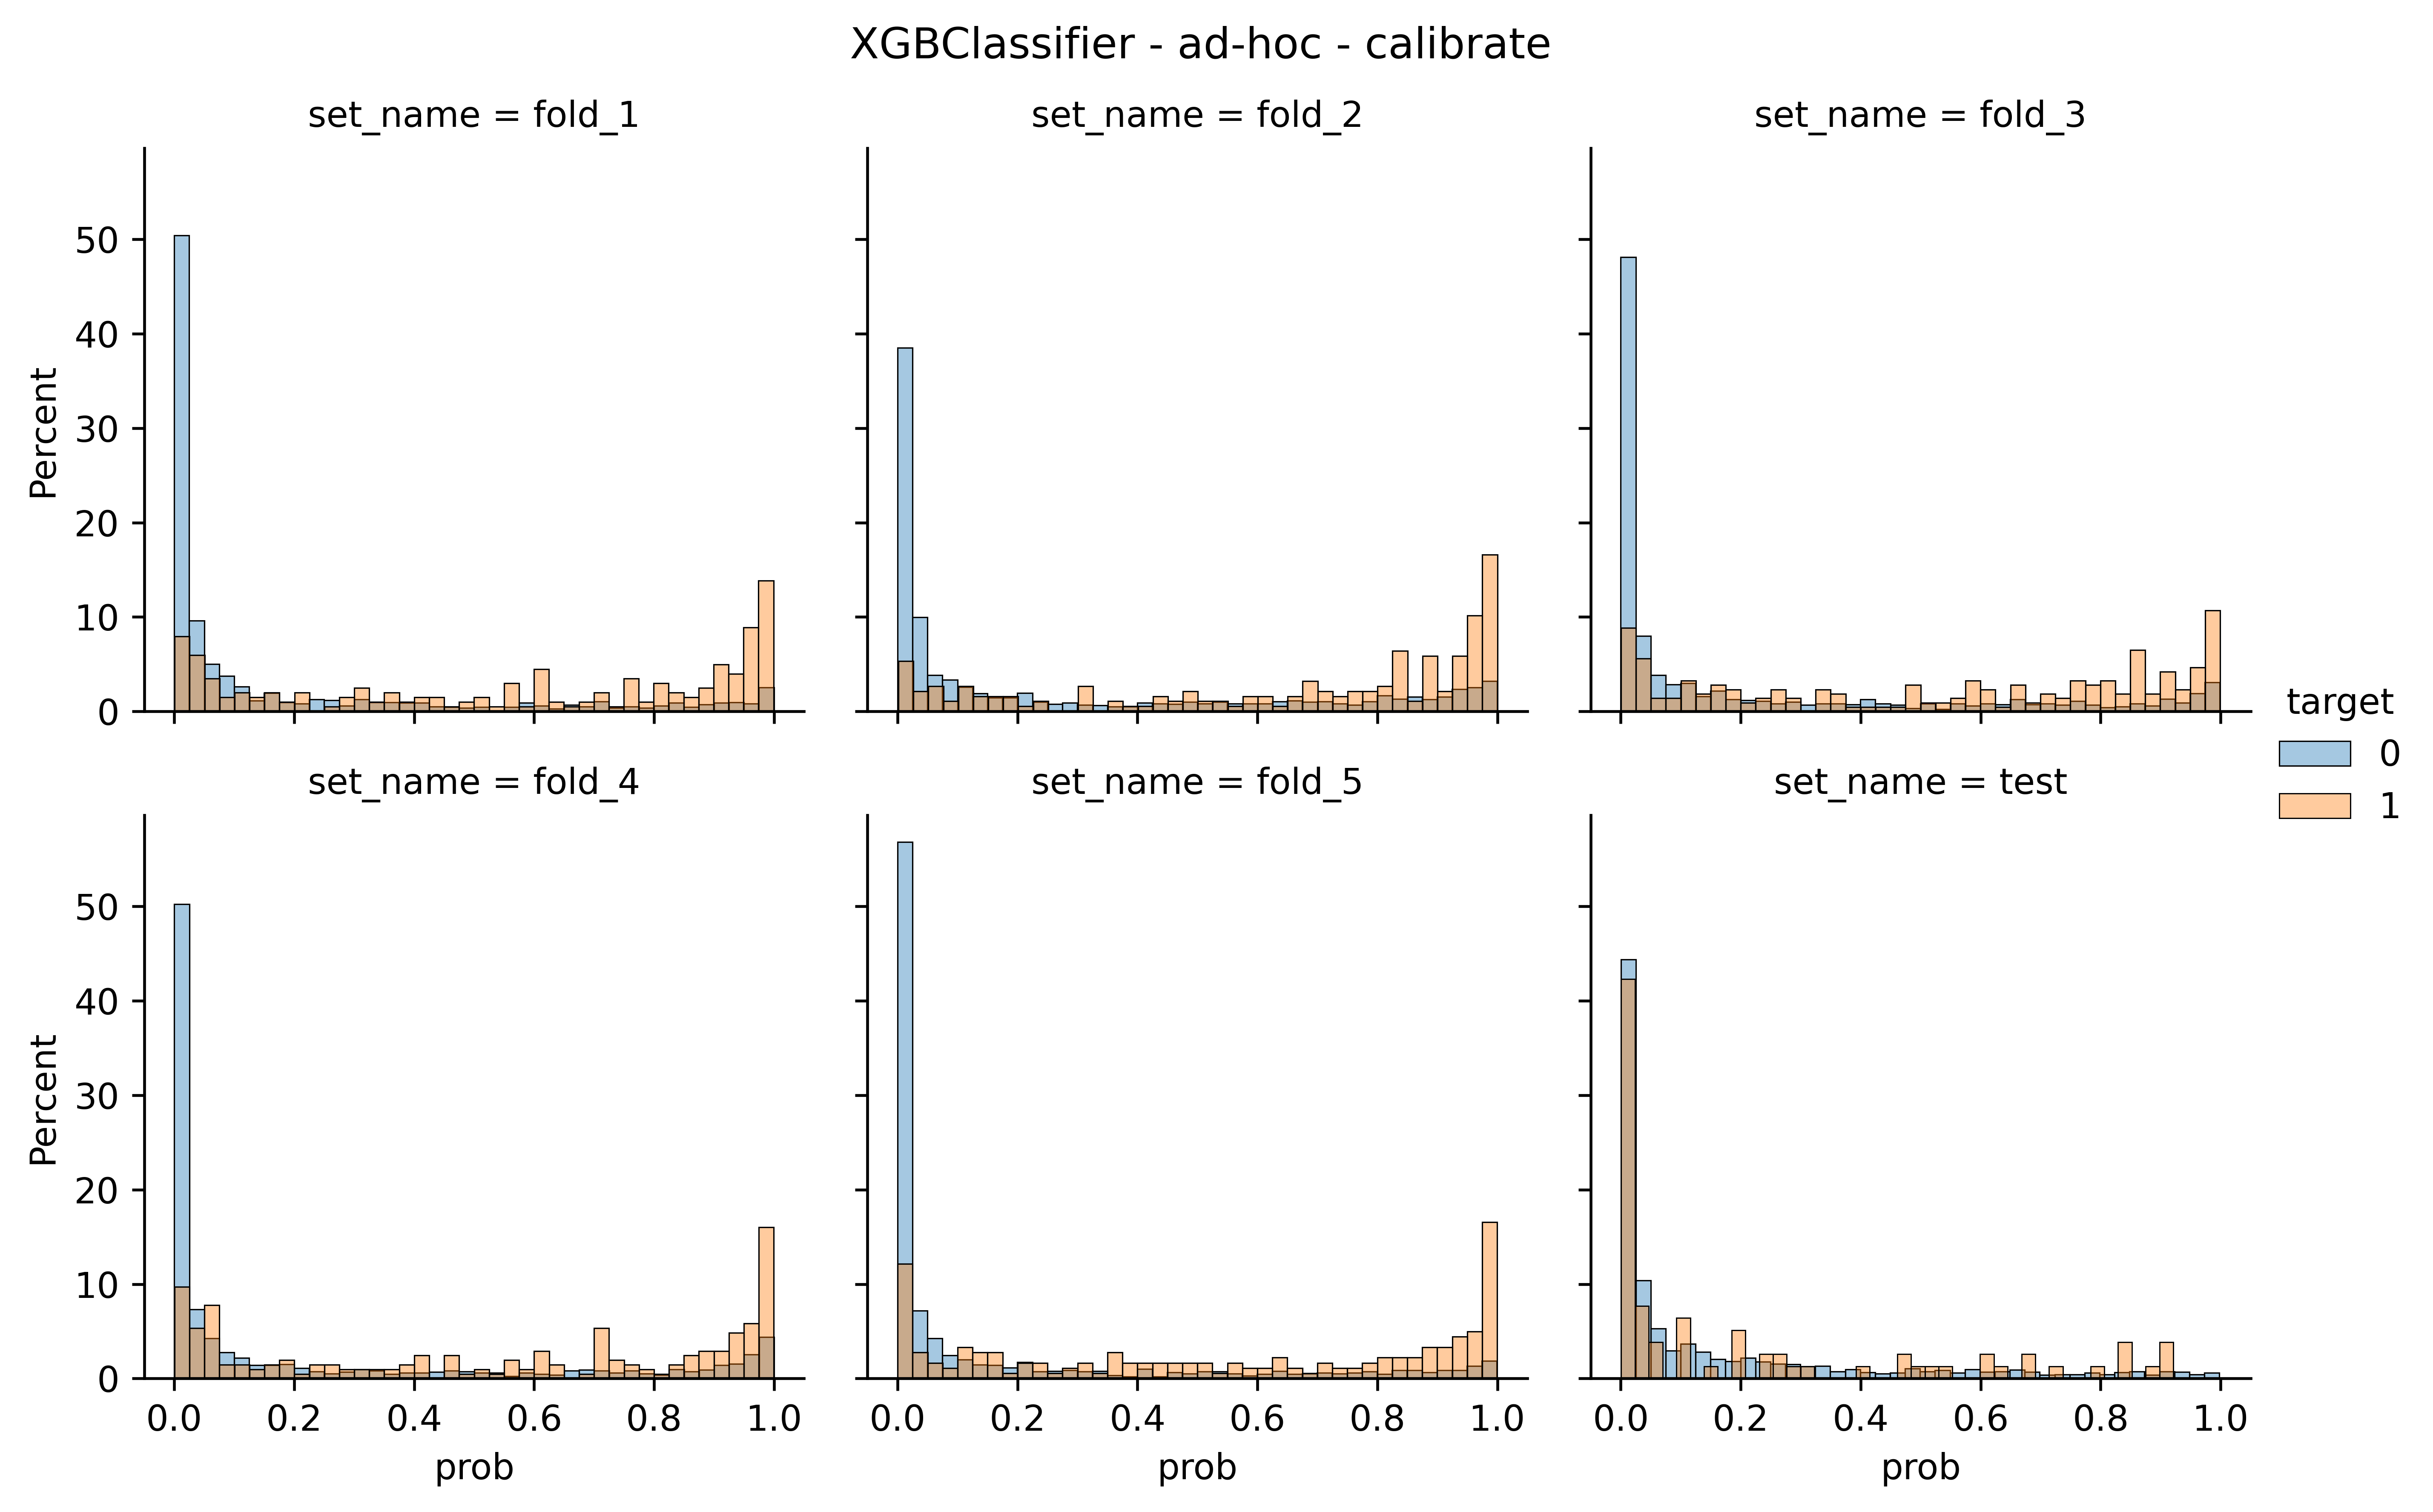
\includegraphics[width=\linewidth]{figures/results/ad-hoc/xgb/2021-12-07_06.29.19.600877__distplot (2).png}
    \end{subfigure}
    \hfill
    \centering
    \begin{subfigure}[b]{0.83\textwidth}
        \centering
        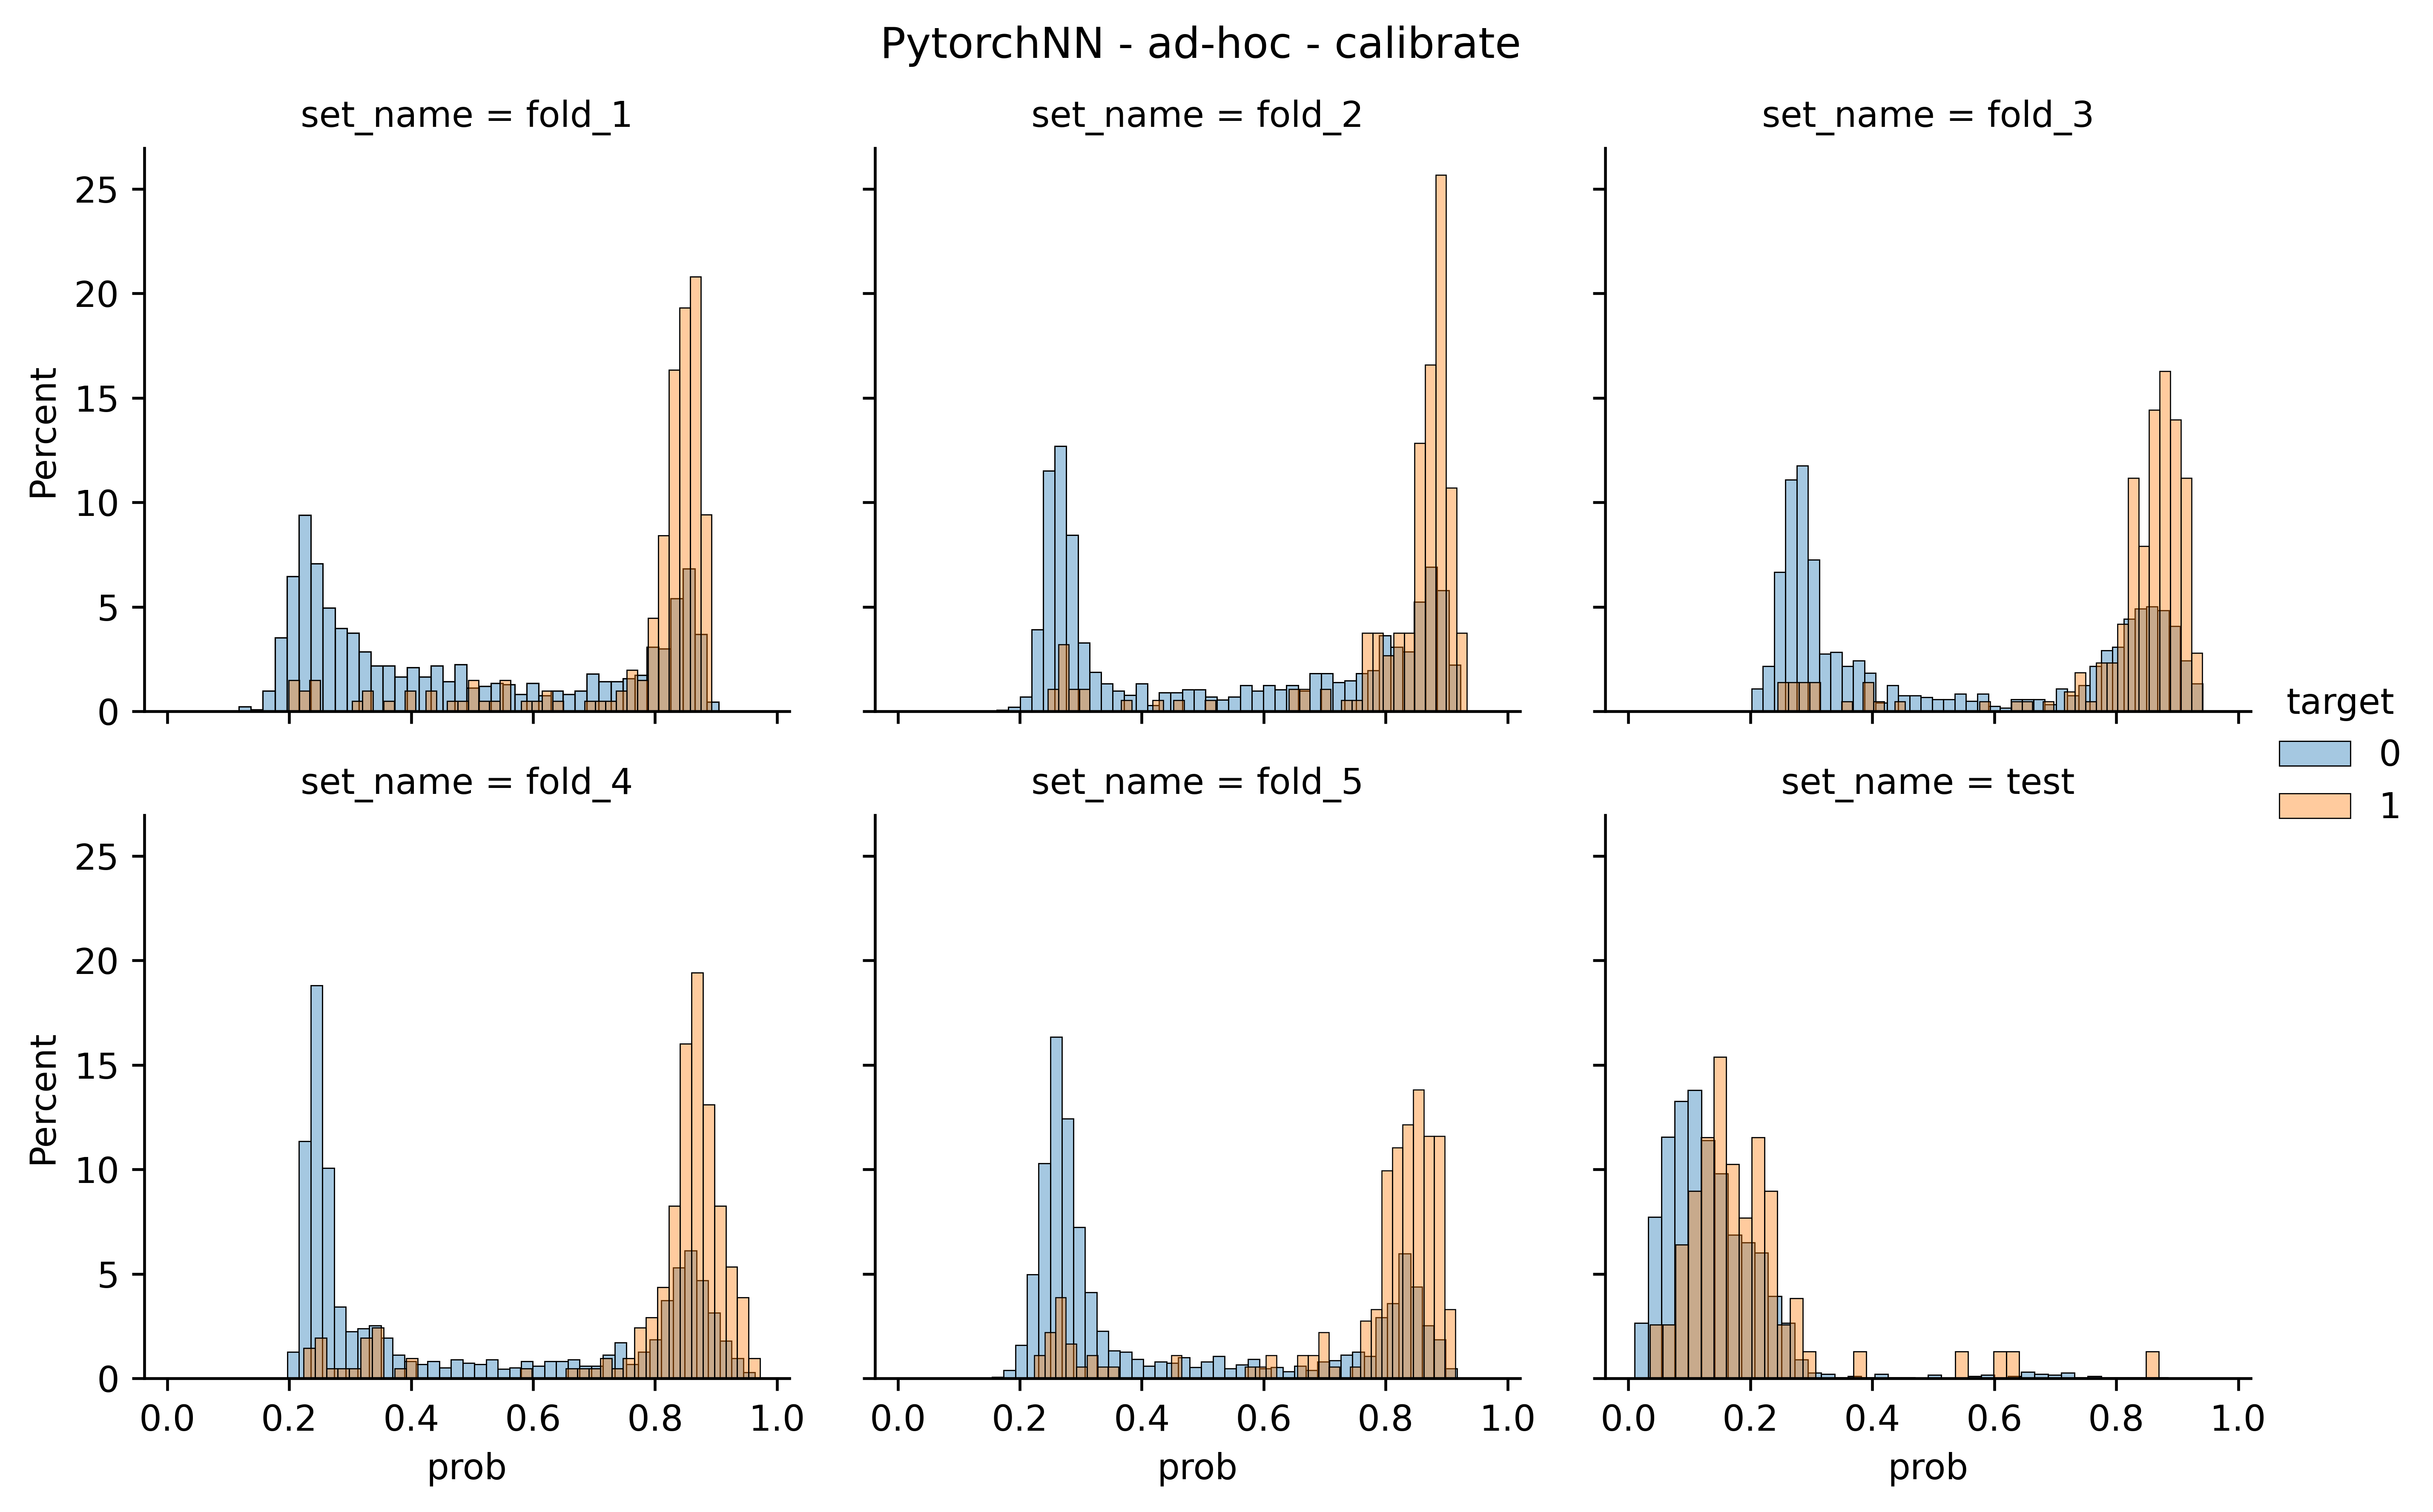
\includegraphics[width=\linewidth]{figures/results/ad-hoc/nn/2021-12-06_17.03.17.314982__distplot.png}
    \end{subfigure}
    \caption{Ad-hoc calibrate}
\end{figure}

\begin{figure}
    \centering
    \begin{subfigure}[b]{0.83\textwidth}
    \includegraphics[width=\linewidth]{figures/results/ad-hoc/lgr/switch_on/turn_to__distplot.png}
    \end{subfigure}
    \hfill
    \centering
    \begin{subfigure}[b]{0.83\textwidth}
        \centering
        \includegraphics[width=\linewidth]{figures/results/ad-hoc/xgb/switch_on/2021-12-07_06.56.08.418411__distplot.png}
    \end{subfigure}
    \hfill
    \centering
    \begin{subfigure}[b]{0.83\textwidth}
        \centering
        \includegraphics[width=\linewidth]{figures/results/ad-hoc/nn/switch_on/2021-12-06_18.44.35.478500__distplot.png}
    \end{subfigure}
    \caption{Ad-hoc switch\_on}
\end{figure}

\begin{figure}
    \centering
    \begin{subfigure}[b]{0.83\textwidth}
    \includegraphics[width=\linewidth]{figures/results/ad-hoc/lgr/take_image/take_image__distplot.png}
    \end{subfigure}
    \hfill
    \centering
    \begin{subfigure}[b]{0.83\textwidth}
        \centering
        \includegraphics[width=\linewidth]{figures/results/ad-hoc/xgb/2021-12-07_07.38.35.967776__distplot.png}
    \end{subfigure}
    \caption{Ad-hoc take\_image}
\end{figure}

\section{Comparación de mejores modelos}
\label{results:comparison}

\section{Tiempos de predicción}
\label{exp:time}

Para un nuevo ejemplo no visto se debe realizar el proceso completo creación de
ventanas, codificación, predicción por parte del clasificador, y posterior
agrupamiento de ventanas para obtener la máxima prioridad. Al incluir los
modelos predictivos en el proceso de grounding heurístico el tiempo necesario
para realizar todas las etapas y obtener el valor de salida del modelo
predictivo es importante durante el proceso de grounding heurístico ya que los
planificadores deben encontrar la solución a la tarea asignada de acuerdo a un
tiempo límite, si este es excedido, ocurre una falla por parte del planificador.
Esto motivo la medición del tiempo de respuesta para los modelos predictivos
comparados en la sección \ref{results:comparison}.

Actualmente la implementación de grounding heurístico en Fast Downward, son
realizadas a nivel de ejemplo. Por lo que la unidad de medida utilizada fueron
\emph{ns/ejemplo}, no obstante también se probaron realizar las predicciones a
nivel de batch con el de determinar que tan prometedor es incluir este cambio en
el algoritmo de grounding heurístico.

\subsection{Predicciones por batch}

\subsection{Predicciones por acción}

\section{Otros experimentos}

Los experimentos presentados en las secciones \ref{exp:ad-hoc}, \ref{exp:wb}, y
\ref{exp:time} fueron aquellos principales y los que nos enfocamos durante la
tesis. No obstante, se intentaron otras vías de análisis que llevaron a 4
experimentos con el fin de lograr aquel modelo que nos permita guiar el proceso
de grounding. A pesar de no lograr resultados concretos fueron parte importante
del trabajo y otorgaron conocimiento invaluable para involucrarse más en el
dominio del problema.

\subsection{Modelos End-to-end}

End-to-end (E2E) models refieren a sistemas complejos representados por un único
modelo neuronal profundo ensamblando las capas de preprocesamiento y como capas
intermedias del modelo. En particular, este tipo de pruebas se realizaron en una
etapa temprana de la tesis donde la idea de generar ventanas de planes relajados
aún no se había investigado. En particular se experimentaron con modelos E2E de
FastText donde agrega una capa neuronal más al modelo de embeddings para que
sean utilizados en clasificación. No obstante se optó por descontinuar estos
experimentos al comenzar ya que fueron experimentos prototipos donde se buscaba
verificar la factibilidad del uso de word embeddings en grounding heurístico.

\subsection{El problema de inclusión sobre planes relajados}

Otra estrategía que utilizamos durante el análisis en la generación de ventanas
de planes relajados, fue plantear el problema de clasificación binaria como uno
multiclase. En lugar de solo 2 clases, manteníamos 4 que representaban la noción
de si una acción estaba incluido en el plan relajado y si eran parte de los good
operators del problema. Es decir, una ventana de plan relajado $w$ y acción $a$
es etiquetada como:

\begin{itemize}
    \item 0: Si $a$ no es good operator y no pertenece a $w$.
    \item 1: Si $a$ no es good operator y pertenece a $w$.
    \item 2: Si $a$ es good operator y no pertenece a $w$.
    \item 3: Si $a$ es good operator y pertenece a $w$.
\end{itemize}

Luego al agrupar por ventanas y acción, consideramos como predicción final la
clase $3$ si al menos una de las ventanas predijo $3$. Caso contrario si para
alguna ventana la predicción fue $2$ predicción del agrupamiento es $2$. Y así
sucesivamente hasta la clase $0$.

\subsection{Mayorización}

La repetición de ejemplos con etiquetas diferentes puede dificultar el
aprendizaje de un modelo, si no son preprocesadas con alguna técnica de
mayorización. Es decir, de entre todas las repeticiones del mismo ejemplo pero
con distintas clases, mantener una sola replica preservando la etiqueta que haya
ocurrido en mayor cantidad. Esta técnica fue aplicada para la codificación por
word embeddings, donde una hipótesis para mejorar la separación de los ejemplos
de entrenamiento fue asignar la etiqueta mayoritaria para todo los vector de
dimensión $D$ (plan relajado, acción) que estén cerca en un rango en
$\mathbb{R}^{D}$.

\subsection{Orden de ventanas como características}

Por último otra implementación que se agregó al sistema y que es un patrón
configurable de las etapas de ejecución es la posibilidad de mantener el orden
en que ocurren las ventanas. Es decir, se tiene

\begin{table}[h!]
\centering
\scalebox{0.9}{
 \begin{tabular}{||c | c | c | c||} 
 \hline
 Plan relajado & Orden de ventana & Acción & Etiqueta \\ [0.5ex] \hline\hline
 %(take_image satellite0 planet5 instrument1 image1)
 {}[] & 1 &{}[] & 1 \\
 {}[] & 2 &{}[] & 1 \\
 {}[] & 3 &{}[] & 1  \\
 ... & ... & ... & ...\\ [1ex] 
 \hline
 \end{tabular}}
 \caption{Ejemplos etiquetados a partir de un plan relajado y una acción}
 \label{tb:matrix_shape}
\end{table}

El objetivo de este agregado es evitar perder la información del orden durante
la separación y se buscaba analizar si es un factor relevante para el
entrenamiento y evaluación.

    \part{Conclusión}
    \chapter{Conclusions and Future Work}
\label{ch:con}
\section{Conclusions}
Typically a conclusions chapter first summarizes the investigated problem and its aims and objectives. It summaries the critical/significant/major findings/results about the aims and objectives that have been obtained by applying the key methods/implementations/experiment set-ups. A conclusions chapter draws a picture/outline of your project's central and the most signification contributions and achievements. 

A good conclusions summary could be approximately 300--500 words long, but this is just a recommendation.

A conclusions chapter followed by an abstract is the last things you write in your project report.

\section{Future work}
This section should refer to Chapter~\ref{ch:results} where the author has reflected their criticality about their own solution. The future work is then sensibly proposed in this section.

\textbf{Guidance on writing future work:} While working on a project, you gain experience and learn the potential of your project and its future works. Discuss the future work of the project in technical terms. This has to be based on what has not been yet achieved in comparison to what you had initially planned and what you have learned from the project. Describe to a reader what future work(s) can be started from the things you have completed. This includes identifying what has not been achieved and what could be achieved. 



A good future work summary could be approximately 300--500 words long, but this is just a recommendation.

    % -------------------------------------------------------------------
    % Bibliography/References
    % -------------------------------------------------------------------
    \bibliographystyle{agsm}
    
    \bibliography{references}
    
    % -------------------------------------------------------------------
    % Appendices
    % -------------------------------------------------------------------
    
\end{document}
